\documentclass[11pt,letterpaper]{article}

% ---------------------------------------------------------------------
%  Paquetes
% ---------------------------------------------------------------------
\usepackage[utf8]{inputenc}
\usepackage[T1]{fontenc}
\usepackage[spanish,es-noshorthands,es-tabla,es-nodecimaldot]{babel}
\usepackage{lmodern}
\usepackage{microtype}
\usepackage[letterpaper,margin=2.3cm,headheight=14pt]{geometry}

\usepackage{amsmath,amssymb,mathtools,bm}
\usepackage{cancel}
\usepackage{booktabs,array}
\usepackage{graphicx}
\usepackage[dvipsnames]{xcolor}
\usepackage{enumitem}
\usepackage{tikz}
\usepackage{listings}
\lstset{language=Python, basicstyle=\ttfamily\footnotesize, breaklines=true,
  columns=fullflexible, keepspaces=true, showstringspaces=false,
  commentstyle=\color{black!60}\itshape, keywordstyle=\bfseries,
  numbers=left, numberstyle=\tiny\color{black!50}, frame=lines,
  literate={á}{{\'a}}1 {é}{{\'e}}1 {í}{{\'i}}1 {ó}{{\'o}}1 {ú}{{\'u}}1
           {Á}{{\'A}}1 {É}{{\'E}}1 {Í}{{\'I}}1 {Ó}{{\'O}}1 {Ú}{{\'U}}1
           {ñ}{{\~n}}1 {Ñ}{{\~N}}1 {ü}{{\"u}}1}
\usetikzlibrary{arrows.meta,positioning,calc}
\usepackage{fancyhdr}
\usepackage{titlesec}
\titleformat*{\subsection}{\normalsize\bfseries}
\titleformat*{\subsubsection}{\normalsize\bfseries\itshape}
\usepackage[hidelinks]{hyperref}

\graphicspath{{figuras/}}
\setlist[enumerate]{itemsep=2pt,topsep=4pt}
\setlength{\parindent}{0pt}
\setlength{\parskip}{4pt}
\setcounter{secnumdepth}{1}

\pagestyle{fancy}
\fancyhf{}
\fancyfoot[C]{\thepage}
\renewcommand{\headrulewidth}{0pt}

% ---------------------------------------------------------------------
%  Macros de notación (la del profesor).
%  Si cambias una notación aquí, cambia en todo el documento.
% ---------------------------------------------------------------------

% Orden de error: \Order{h^2}  ->  O(h^2)
\newcommand{\Order}[1]{\mathcal{O}\!\left(#1\right)}

% Diferencial recto y derivada temporal: \ddt{u} -> du/dt
\newcommand{\dd}{\mathrm{d}}
\newcommand{\ddt}[1]{\frac{\dd #1}{\dd t}}

% Valor EXACTO en un nodo:   \uex{\ell}  -> u(t_\ell)
% Valor NUMÉRICO en un nodo: u_\ell      (se escribe directo)
\newcommand{\uex}[1]{u(t_{#1})}

% Punto medio entre nodos: t_{\lmed} -> t_{\ell+1/2}
\newcommand{\lmed}{\ell+1/2}
% Igual con índice n (notación del examen): t_{\nmed} -> t_{n+1/2}
\newcommand{\nmed}{n+1/2}

% Punto fijo / solución particular
\newcommand{\ufijo}{u^{*}}

% Orden de convergencia global / local (Sesión 02)
\newcommand{\OCG}{\mathrm{OCG}}
\newcommand{\OCL}{\mathrm{OCL}}

% Matrices y vectores (para las Partes II–IV)
\newcommand{\mat}[1]{\mathbf{#1}}
\newcommand{\vect}[1]{\bm{#1}}
\newcommand{\tridiag}{\operatorname{tridiag}}
\newcommand{\keff}{k_{\mathrm{ef}}}

% ---------------------------------------------------------------------
%  Estructura: partes, problemas, incisos, pasos
% ---------------------------------------------------------------------

\makeatletter
% \parte{I}{Decaimiento radiactivo}{20}
% Cada parte y cada problema empiezan en hoja nueva; el primer problema de
% una parte se queda en la misma hoja que el título de la parte.
\newif\ifrecienparte
\newcommand{\parte}[3]{%
  \clearpage\phantomsection\global\recienpartetrue
  \section*{Parte #1. #2 (#3 pts)}%
  \addcontentsline{toc}{section}{Parte #1. #2}%
  \markboth{Parte #1. #2}{Parte #1. #2}}

% \problema{3}{Decaimiento con fuente}{6}
% Se puede referir con  Problema~\ref{prob:3}
\newcommand{\problema}[3]{%
  \ifrecienparte\global\recienpartefalse\else\clearpage\fi
  \phantomsection
  \subsection*{Problema #1. #2\hfill[#3 pts]}%
  \addcontentsline{toc}{subsection}{Problema #1. #2}%
  \protected@edef\@currentlabel{#1}%
  \label{prob:#1}}

% \inciso{a}{Esquema CN con fuente}
% Si el título lleva matemáticas, usa \texorpdfstring{$...$}{texto} para el índice del PDF.
\newcommand{\inciso}[2]{%
  \phantomsection
  \subsubsection*{(#1) #2}%
  \addcontentsline{toc}{subsubsection}{(#1) #2}}
\makeatother

% \paso{1}{Generación del mallado}
\newcommand{\paso}[2]{\par\medskip\textbf{Paso #1.} \textit{#2}\par\smallskip}

% ---------------------------------------------------------------------
%  Notas dentro del texto (sin cajas)
% ---------------------------------------------------------------------

% Enunciado del problema
\newenvironment{enunciado}{\par}{\par\medskip}

% porque / ojo / leveque: la explicación va directo como párrafo normal, sin título.
% (El título opcional, p. ej. \begin{porque}[...], se ignora.)
\newenvironment{porque}[1][]{\par}{\par}
\newenvironment{ojo}[1][]{\par}{\par}
\newenvironment{leveque}[1][]{\par}{\par}

% Resultado final destacado: \resultado{ ecuación }
\newcommand{\resultado}[1]{\[\boxed{\displaystyle #1}\]}

% Problema aún sin resolver
\newcommand{\pendiente}{\par\textit{Solución pendiente.}\par}

% ---------------------------------------------------------------------
%  Material generado por Python (no rompe la compilación si falta)
% ---------------------------------------------------------------------
% \figurapython{p3_solucion}{Pie de figura}{fig:p3sol}{0.8}
\newcommand{\figurapython}[4]{%
  \begin{figure}[htbp]\centering
  \IfFileExists{figuras/#1.pdf}{%
    \includegraphics[width=#4\textwidth]{figuras/#1.pdf}}{%
    \fbox{\parbox{0.7\textwidth}{\centering\small
      Falta \texttt{figuras/#1.pdf}.\\ Ejecuta \texttt{make figs} en la raíz.}}}
  \caption{#2}\label{#3}
  \end{figure}}

% \tablapython{p3_d}  — inserta latex/tablas/p3_d.tex
\newcommand{\tablapython}[1]{%
  \IfFileExists{tablas/#1.tex}{\input{tablas/#1.tex}}{%
    \fbox{\small Falta \texttt{tablas/#1.tex}: ejecuta \texttt{make figs}.}}}

% Respuesta de opción múltiple / conceptual: \respuesta{b) porque ...}
% Si se deja vacía, \respuesta{} imprime una línea en blanco.
\newcommand{\respuesta}[1]{%
  \par\smallskip\textbf{Respuesta:}~%
  \if\relax\detokenize{#1}\relax\rule{3cm}{0.4pt}\else #1\fi\par}


\newcommand{\titulodoc}{Computadoras en la Ingeniería Nuclear}
\newcommand{\subtitulodoc}{}
\newcommand{\autordoc}{Edgar Solano Castrejón}
\newcommand{\institucion}{Instituto Politécnico Nacional\\Escuela Superior de Física y Matemáticas}
% >>> Cambia esta URL por la de tu repositorio de GitHub
\newcommand{\repoCIN}{https://github.com/USUARIO/CIN-Problemas}
\newcommand{\programa}{Maestría en Ciencias Fisicomatemáticas (LIE: Ingeniería Nuclear)}

\begin{document}

\begin{center}
  {\large\bfseries \institucion\par}
  \medskip
  Programa de Posgrado --- \programa\par
  \smallskip
  \titulodoc: \subtitulodoc\par
  \smallskip
  \autordoc\par
  \smallskip
  \today
\end{center}

\bigskip

\begin{center}
\begin{tabular}{lcc}\toprule
Parte & Tema & Puntos\\\midrule
I   & Decaimiento radiactivo (sin y con fuente) & 20\\
II  & Difusión estacionaria 1D y 2D             & 20\\
III & Difusión dependiente del tiempo           & 15\\
IV  & Problemas de valores propios              & 20\\
V   & Preguntas conceptuales                    & 10\\
VI  & Opción múltiple (20 reactivos)            & 15\\\bottomrule
\end{tabular}
\end{center}



\parte{I}{Decaimiento radiactivo}{20}

% !TeX root = ../main.tex
\problema{1}{Decaimiento sin fuente: tres esquemas de un paso}{6}

\begin{enunciado}
	Sea $\dfrac{\dd N}{\dd t} = -\lambda N$, $N(0) = N_0 = 100$, con $\lambda = \tfrac12$ y $h = \tfrac12$.
	\begin{enumerate}[label=(\alph*)]
		\item Deduzca los esquemas de Euler explícito, Euler implícito y Crank--Nicolson (CN)
		usando diferencias divididas de primer orden y el promedio de $f$ en $t_n$ y $t_{n+1}$.
		\item Calcule $N_1 \approx N(h)$ con cada esquema y el error absoluto respecto a la solución exacta.
		\item Obtenga el factor de amplificación $R(z)$, con $z = -\lambda h$, de cada esquema y
		determine su región de estabilidad. ¿Qué ocurre con $R$ cuando $\lambda h \to \infty$?
	\end{enumerate}
\end{enunciado}

\subsubsection*{Solución}
\[
\ddt{N} = -\lambda\,N(t), \qquad N(0) 	= N_0,
\]
Solución exacta es:
\[
\frac{\dd N}{\dd t} = -\lambda N
\;\Longrightarrow\; N(t) = N_0\,e^{-\lambda t} = 100\,e^{-t/2}
\]

\inciso{a}{Deduccion de los tres esquemas}


\paso{1}{Generación del mallado}
Se discretiza el tiempo con paso $h$:
\[
t_n = n h, \qquad n = 0, 1, 2, \dots, \qquad N_n \approx N(t_n).
\]

\textbf{Esquema 1: Euler explícito (diferencia dividida progresiva)}

\paso{2}{Colocación de la EDO en $t = t_n$}
\[
\left.\ddt{N}\right|_{t_n} = -\lambda\,N(t_n).
\]

\paso{3}{Sustituir la derivada por la diferencia progresiva}
Taylor alrededor de $t_n$:
\[
N(t_n + h) = N(t_n) + h\,N'(t_n) + \frac{h^2}{2!}\,N''(t_n) + \Order{h^3}.
\]
Despejando $N'(t_n)$:
\[
N'(t_n) = \frac{N(t_n + h) - N(t_n)}{h} - \frac{h}{2}\,N''(t_n) + \Order{h^2}.
\]
El término ($-\frac{h}{2}\,N''(t_n) + \Order{h^2}$) es el error de truncamiento de la diferencia
dividida, y es de orden $\Order{h}$. Sustituyendo en la EDO:
\[
\frac{N(t_{n+1}) - N(t_n)}{h} - \frac{h}{2}\,N''(t_n) + \Order{h^2} = -\lambda\,N(t_n).
\]
Quitamos el error de truncamiento y llamamos $N_n$ a la aproximación de $N(t_n)$:
\[
\frac{N_{n+1} - N_n}{h} = -\lambda\,N_n
\;\Longrightarrow\;
N_{n+1} - N_n = -\lambda h\,N_n .
\]

\resultado{N_{n+1} = (1 - \lambda h)\,N_n, \qquad n = 0, 1, 2, \dots}

Es explicito $N_{n+1}$ porque lo calculamos con $N_n$.

Es importante resaltar que $N(t_n) \neq N_n$. Al quitar el $\Order{h}$ ya no es el valor exacto en el nodo ya es una aproximación $N(t_n) \approx N_n$. Aqui lo que nos esta diciendo es que no se "quita" asi magicamente sino que se esta acumulando el error paso a pasao

\textbf{De forma general queda}
\begin{align*}
	N_1 &= (1 - \lambda h)\,N_0\\
	N_2 &= (1 - \lambda h)^2\,N_0\\
	&\;\;\vdots\\
	N_n &= (1 - \lambda h)^n\,N_0
\end{align*}


\textbf{Esquema 2: Euler implícito (diferencia dividida regresiva)}

\paso{2}{Colocación de la EDO en $t = t_n$}
\[
\left.\ddt{N}\right|_{t_n} = -\lambda\,N(t_n).
\]

\paso{3}{Sustituir la derivada por la diferencia regresiva}
Taylor alrededor de $t_n$, ahora hacia atrás:
\[
N(t_n - h) = N(t_n) - h\,N'(t_n) + \frac{h^2}{2!}\,N''(t_n) + \Order{h^3}.
\]
Despejando $N'(t_n)$:
\[
N'(t_n) = \frac{N(t_n) - N(t_n - h)}{h} + \frac{h}{2}\,N''(t_n) + \Order{h^2}.
\]
El error de truncamiento es $+\frac{h}{2}\,N''(t_n) + \Order{h^2}$, y nos damos cuenta que es de signo opuesto a la progresiva. Sustituyendo en la EDO y haciendo $N(t_n) \approx N_n$
\begin{align*}
	\frac{N_n - N_{n-1}}{h} &= -\lambda\,N_n\\
	N_n - N_{n-1} &= -\lambda h\,N_n\\
	N_n + \lambda h\,N_n &= N_{n-1}
	\;\Longrightarrow\; N_n\,(1 + \lambda h) = N_{n-1}
\end{align*}

\resultado{N_n = \frac{1}{1 + \lambda h}\,N_{n-1}, \qquad n = 1, 2, \dots}

\textbf{Caso general.}
\begin{align*}
	N_1 &= \frac{N_0}{1 + \lambda h}\\
	N_2 &= \frac{N_0}{(1 + \lambda h)^2}\\
	&\;\;\vdots\\
	N_n &= \frac{N_0}{(1 + \lambda h)^n}
\end{align*}

\paragraph{Esquema 3: Crank--Nicolson}

\paso{2}{Colocación de la EDO en $t_{\nmed}$}
$t_{\nmed} = t_n + h/2$:
\[
\left.\ddt{N}\right|_{t_{\nmed}} = -\lambda\,N(t_{\nmed}).
\]

Aquí la EDO no lo colocamos en un nodo entero ya que si lo hacemos daria
$\dfrac{N_{n+1} - N_{n-1}}{2h}$, con 2 incógnitas que no se conocen


%\paso{3}{Sustituir la derivada por la diferencia centrada}
%Se hacen dos desarrollos de Taylor alrededor de $t_{\nmed}$, con
%$t_{n+1} = t_{\nmed} + \tfrac{h}{2}$ y $t_n = t_{\nmed} - \tfrac{h}{2}$:
%\begin{align*}
%	N(t_{n+1}) &= N(t_{\nmed}) + \frac{h}{2}\,N'(t_{\nmed})
%	+ \frac{1}{2!}\left(\frac{h}{2}\right)^2 N''(t_{\nmed})
%	+ \frac{1}{3!}\left(\frac{h}{2}\right)^3 N'''(t_{\nmed}) + \Order{h^4}\\
%	N(t_n)     &= N(t_{\nmed}) - \frac{h}{2}\,N'(t_{\nmed})
%	+ \frac{1}{2!}\left(\frac{h}{2}\right)^2 N''(t_{\nmed})
%	- \frac{1}{3!}\left(\frac{h}{2}\right)^3 N'''(t_{\nmed}) + \Order{h^4}
%\end{align*}

\paso{3}{Sustituir la derivada por la diferencia centrada (paso $h/2$)}
Se hacen dos desarrollos de Taylor alrededor de $t_{\nmed}$, con
$t_{n+1} = t_{\nmed} + \tfrac{h}{2}$ y $t_n = t_{\nmed} - \tfrac{h}{2}$.
Tomare hasta $N^{(5)}$ para ver que terminos se van a cancelar y las derivadas estan evaluadas en $t_{\nmed}$
\begin{align*}
	N(t_{n+1}) &= N(t_{\nmed}) + \frac{h}{2}\,N'
	+ \frac{1}{2!}\left(\frac{h}{2}\right)^2 N''
	+ \frac{1}{3!}\left(\frac{h}{2}\right)^3 N'''
	+ \frac{1}{4!}\left(\frac{h}{2}\right)^4 N^{(4)}
	+ \frac{1}{5!}\left(\frac{h}{2}\right)^5 N^{(5)} + \Order{h^6}\\
	N(t_n)     &= N(t_{\nmed}) - \frac{h}{2}\,N'
	+ \frac{1}{2!}\left(\frac{h}{2}\right)^2 N''
	- \frac{1}{3!}\left(\frac{h}{2}\right)^3 N'''
	+ \frac{1}{4!}\left(\frac{h}{2}\right)^4 N^{(4)}
	- \frac{1}{5!}\left(\frac{h}{2}\right)^5 N^{(5)} + \Order{h^6}
\end{align*}

Restando las dos ecuacioneslos terminos pares se cancelan y los otros se duplican
\begin{align*}
	N(t_{n+1}) - N(t_n)
	&= \bigl[N(t_{\nmed}) - N(t_{\nmed})\bigr]
	+ \left[\frac{h}{2} + \frac{h}{2}\right] N'
	+ \Bigl[\cancel{\tfrac{1}{2!}\left(\tfrac{h}{2}\right)^2 N''} - \cancel{\tfrac{1}{2!}\left(\tfrac{h}{2}\right)^2 N''}\Bigr]\\
	&\quad + \frac{1}{3!}\left[\left(\frac{h}{2}\right)^3 + \left(\frac{h}{2}\right)^3\right] N'''
	+ \Bigl[\cancel{\tfrac{1}{4!}\left(\tfrac{h}{2}\right)^4 N^{(4)}} - \cancel{\tfrac{1}{4!}\left(\tfrac{h}{2}\right)^4 N^{(4)}}\Bigr]\\
	&\quad + \frac{1}{5!}\left[\left(\frac{h}{2}\right)^5 + \left(\frac{h}{2}\right)^5\right] N^{(5)} + \Order{h^6}
\end{align*}
entonces
\[
N(t_{n+1}) - N(t_n) = h\,N'(t_{\nmed}) + \frac{h^3}{24}\,N'''(t_{\nmed}) + \frac{h^5}{1920}\,N^{(5)}(t_{\nmed}) + \cdots
\]
\[
= h\,N'(t_{\nmed}) + \frac{h^3}{24}\,N'''(t_{\nmed}) + \Order{h^5}
\]

Despejando $N'(t_{\nmed})$
\begin{align*}
	h\,N'(t_{\nmed}) &= N(t_{n+1}) - N(t_n) - \frac{h^3}{24}\,N'''(t_{\nmed}) - \Order{h^5}\\
	N'(t_{\nmed}) &= \frac{N(t_{n+1}) - N(t_n)}{h} - \frac{h^2}{24}\,N'''(t_{\nmed}) + \Order{h^4}
\end{align*}

Sumando las ecuaciones
\begin{align*}
	N(t_{n+1}) + N(t_n)
	&= 2\,N(t_{\nmed})
	+ \Bigl[\cancel{\tfrac{h}{2}\,N'} - \cancel{\tfrac{h}{2}\,N'}\Bigr]
	+ \frac{2}{2!}\left(\frac{h}{2}\right)^2 N''\\
	&\quad + \Bigl[\cancel{\tfrac{1}{3!}\left(\tfrac{h}{2}\right)^3 N'''} - \cancel{\tfrac{1}{3!}\left(\tfrac{h}{2}\right)^3 N'''}\Bigr]
	+ \frac{2}{4!}\left(\frac{h}{2}\right)^4 N^{(4)} + \Order{h^6}
\end{align*}

\[
\frac{N(t_n) + N(t_{n+1})}{2} = N(t_{\nmed}) + \frac{h^2}{8}\,N''(t_{\nmed}) + \frac{h^4}{384}\,N^{(4)}(t_{\nmed}) + \cdots
= N(t_{\nmed}) + \frac{h^2}{8}\,N''(t_{\nmed}) + \Order{h^4}
\]
Despejando $N(t_{\nmed})$:
\[
N(t_{\nmed}) = \frac{N(t_n) + N(t_{n+1})}{2} - \frac{h^2}{8}\,N''(t_{\nmed}) + \Order{h^4}
\]

Los errores de truncamiento son entonces $\Order{h^2}$ 
\\
Sustituyendo en la EDO
$N'(t_{\nmed}) = -\lambda\,N(t_{\nmed})$
\[
\frac{N_{n+1} - N_n}{h} = -\lambda\,\frac{N_n + N_{n+1}}{2}.
\]

Algebra...
\begin{align*}
	2\left(N_{n+1} - N_n\right) &= -\lambda h\,N_n - \lambda h\,N_{n+1}\\
	2\,N_{n+1} + \lambda h\,N_{n+1} &= 2\,N_n - \lambda h\,N_n\\
	N_{n+1}\left(2 + \lambda h\right) &= N_n\left(2 - \lambda h\right)
\end{align*}

\resultado{N_{n+1} = \frac{2 - \lambda h}{2 + \lambda h}\,N_n
	= \frac{1 - \frac{\lambda h}{2}}{1 + \frac{\lambda h}{2}}\,N_n, \qquad n = 0, 1, 2, \dots}

su truncamiento es $\Order{h^2}$

\textbf{Caso general.}
\[
N_n = \left(\frac{2 - \lambda h}{2 + \lambda h}\right)^n N_0 .
\]

\begin{center}
	\begin{tabular}{lcccc}\toprule
		Esquema & Colocación & Diferencia & Formula & Truncamiento\\\midrule
		Euler explícito & $t_n$    & progresiva          & $N_{n+1} = (1 - \lambda h)\,N_n$                          & $\Order{h}$\\[2pt]
		Euler implícito & $t_n$    & regresiva           & $N_n = \dfrac{N_{n-1}}{1 + \lambda h}$                    & $\Order{h}$\\[6pt]
		Crank--Nicolson & $t_{\nmed}$ & centrada & $N_{n+1} = \dfrac{2 - \lambda h}{2 + \lambda h}\,N_n$      & $\Order{h^2}$\\\bottomrule
	\end{tabular}
\end{center}

\textbf{Error local y error global de los tres esquemas}


Forma común de los tres esquemas
Con $z = -\lambda h$ para los tres casos $N_{n+1} = R(z)\,N_n$
\begin{align*}
	\text{Euler explícito:}\quad & N_{n+1} = (1 - \lambda h)\,N_n = (1 + z)\,N_n, && R_{\mathrm{FE}}(z) = 1 + z\\
	\text{Euler implícito:}\quad & N_{n+1} = \frac{N_n}{1 + \lambda h} = \frac{N_n}{1 - z}, && R_{\mathrm{BE}}(z) = \frac{1}{1 - z}\\
	\text{Crank--Nicolson:}\quad & N_{n+1} = \frac{2 - \lambda h}{2 + \lambda h}\,N_n = \frac{2 + z}{2 - z}\,N_n, && R_{\mathrm{CN}}(z) = \frac{2 + z}{2 - z}
\end{align*}
La solución exacta es $N(t)=N_0\,e^{-\lambda t}$. Evaluada en $t_{n+1}=t_n+h$:
\begin{align*}
	N(t_{n+1}) &= N_0\,e^{-\lambda (t_n+h)}\\
	&= e^{-\lambda h}\,N_0\,e^{-\lambda t_n}\\
	&= e^{-\lambda h}\,N(t_n)
	= e^{z}\,N(t_n),
\end{align*}
es decir,
\begin{equation}\label{eq:p01_paso}
	N(t_{n+1}) = e^{z}\,N(t_n), \qquad z=-\lambda h .
\end{equation}
$R(z)$ debe parecerse a $e^{z}$ y su parecido mide el error de un paso

Definiciones
\begin{itemize}
	\item Error de truncamiento: error de la fórmula con que se aproxima la derivada
	\item Error local: error cometido en un solo paso suponiendo exacta la solución en el instante anterior,
	\item Error global: error acumulado en un tiempo final fijo $T$, con $n = T/h$ pasos
\end{itemize}

\inciso{b}{\texorpdfstring{Cálculo de $N_1$ y error absoluto}{Cálculo de N1 y error absoluto}}

Con $\lambda = \tfrac12$ y $h = \tfrac12$:
\[
\lambda h = \frac12\cdot\frac12 = \frac14, \qquad t_1 = 1\cdot h = \frac12 
\]

\textbf{Solución exacta:}
\[
N(h) = N_0\,e^{-\lambda h} = 100\,e^{-1/4} \approx 77.880078 
\]

\textbf{Euler explícito} ($n = 0$): $N_1 = (1 - \lambda h)\,N_0$
\[
N_1 = \left(1 - \tfrac14\right)(100) = \tfrac34(100) = 75 
\]

\textbf{Euler implícito} ($n = 1$): $N_1 = \dfrac{N_0}{1 + \lambda h}$
\[
N_1 = \frac{100}{1 + \frac14} = \frac{100}{5/4} = 80
\]

\textbf{Crank--Nicolson} ($n = 0$): $N_1 = \dfrac{2 - \lambda h}{2 + \lambda h}\,N_0$
\[
N_1 = \frac{2 - \frac14}{2 + \frac14}\,(100) = \frac{7/4}{9/4}\,(100) = \frac{7}{9}\,(100) = \frac{700}{9} \approx 77.777778
\]

Error absoluto $|N(h) - N_1|$
\begin{align*}
	\text{Euler explícito:}\quad & |100\,e^{-1/4} - 75| \approx 2.880078\\
	\text{Euler implícito:}\quad & |100\,e^{-1/4} - 80| \approx 2.119922\\
	\text{Crank--Nicolson:}\quad & \left|100\,e^{-1/4} - \tfrac{700}{9}\right| \approx 0.102301
\end{align*}

Comparación:
\begin{center}
	\begin{tabular}{lccc}\toprule
		Esquema & $N_1$ & exacta & $|N(h) - N_1|$\\\midrule
		Euler explícito & 75 & 77.880078 & 2.880078\\
		Euler implícito & 80 & 77.880078 & 2.119922\\
		Crank--Nicolson & $77.777778$ & 77.880078 & 0.102301\\\bottomrule
	\end{tabular}
\end{center}

Euler explícito subestima y Euler implícito sobreestima esto porque tienen el mismo orden de error a diferencia de Crank--Nicolson tiene un error menor.

\inciso{c}{\texorpdfstring{Factor de amplificación $R(z)$ y estabilidad}{Factor de amplificación R(z) y estabilidad}}

Los tres esquemas tienen la forma
\[
N_{n+1} = R(z)\,N_n \;\Longrightarrow\; N_n = R(z)^n\,N_0, \qquad z = -\lambda h .
\]
La solución exacta cumple
\[
N(t_{n+1}) = N_0\,e^{-\lambda (t_n + h)} = e^{-\lambda h}\,N(t_n) = e^{z}\,N(t_n),
\]
así que $R(z)$ es la aproximación de cada esquema a $e^{z}$.

\textbf{Obtención de $R(z)$.} Se usan las fórmulas del inciso (a) y $\lambda h = -z$:
\begin{align*}
	\text{Euler explícito:}\quad & N_{n+1} = (1 - \lambda h)\,N_n = (1 + z)\,N_n \;\Longrightarrow\; R_{\mathrm{FE}}(z) = 1 + z,\\
	\text{Euler implícito:}\quad & N_{n+1} = \frac{N_n}{1 + \lambda h} = \frac{N_n}{1 - z} \;\Longrightarrow\; R_{\mathrm{BE}}(z) = \frac{1}{1 - z},\\
	\text{Crank--Nicolson:}\quad & N_{n+1} = \frac{2 - \lambda h}{2 + \lambda h}\,N_n = \frac{2 + z}{2 - z}\,N_n \;\Longrightarrow\; R_{\mathrm{CN}}(z) = \frac{2 + z}{2 - z} = \frac{1 + z/2}{1 - z/2} .
\end{align*}

\textbf{Estabilidad absoluta.} Como $N_n = R^n N_0$, si $|R| > 1$ entonces $|N_n|$ crece sin límite
al avanzar en el tiempo, aunque la solución exacta decae. Si $|R| \le 1$ no crece. Por eso el esquema es
\textbf{estable} si
\[
|R(z)| \le 1 ,
\]
y la región de estabilidad es el conjunto de valores $z$ que cumplen esa desigualdad

\textbf{Con los datos del problema} ($\lambda h = \tfrac14$, $z = -\tfrac14$):
\[
R_{\mathrm{FE}} = 1 - \frac14 = \frac34, \qquad
R_{\mathrm{BE}} = \frac{1}{1 + \frac14} = \frac45, \qquad
R_{\mathrm{CN}} = \frac{2 - \frac14}{2 + \frac14} = \frac79 \approx 0.777778, \qquad
e^{-1/4} \approx 0.778801 .
\]
Los tres cumplen $|R| < 1$ y están dentro de su región de estabilidad

\textbf{Comportamiento cuando $\lambda h \to \infty$} ($z \to -\infty$, donde $e^{z} \to 0$).

\textbf{Euler explícito.}
\begin{align*}
	\lim_{\lambda h \to \infty} R_{\mathrm{FE}} &= \lim_{\lambda h \to \infty} \left(1 - \lambda h\right) = -\infty
\end{align*}

\textbf{Euler implícito.}
\begin{align*}
	\lim_{\lambda h \to \infty} R_{\mathrm{BE}} &= \lim_{\lambda h \to \infty} \frac{1}{1 + \lambda h} = 0
\end{align*}

\textbf{Crank--Nicolson.} Dividimos numerador y denominador entre $\lambda h$:
\begin{align*}
	\lim_{\lambda h \to \infty} R_{\mathrm{CN}}
	&= \lim_{\lambda h \to \infty} \frac{2 - \lambda h}{2 + \lambda h}\\
	&= \lim_{\lambda h \to \infty} \frac{\frac{2}{\lambda h} - 1}{\frac{2}{\lambda h} + 1}\\
	&= \frac{0 - 1}{0 + 1}\\
	&= -1
\end{align*}
\begin{center}
	\begin{tabular}{lccp{7cm}}\toprule
		Esquema & $\displaystyle\lim_{z \to -\infty} R(z)$ & Comportamiento\\\midrule
		Euler explícito & $-\infty$ & inestable: $|R|>1$, $|N_n|$ crece oscilando\\
		Euler implícito & $0$       & estable pero va a cero rapido\\
		Crank--Nicolson & $-1$      & estable ($|R|<1$) pero oscila \\\bottomrule
	\end{tabular}
\end{center}

Tabule los resultados en excel para diferentes valores de $\lambda h$ 
\begin{center}
	\begin{tabular}{cccccc}\toprule
		$\lambda h$ & $h$ & $R_{\mathrm{FE}}$ & $R_{\mathrm{BE}}$ & $R_{\mathrm{CN}}$ & $e^{-\lambda h}$\\\midrule
		$\tfrac14$ & $\tfrac12$ & $\tfrac34$ & $\tfrac45$ & $\tfrac79 \approx 0.777778$ & $0.778801$\\
		$1$ & $2$ & $0$ & $\tfrac12$ & $\tfrac13 \approx 0.333333$ & $0.367879$\\
		$2$ & $4$ & $-1$ & $\tfrac13 \approx 0.333333$ & $0$ & $0.135335$\\
		$3$ & $6$ & $-2$ & $\tfrac14$ & $-\tfrac15 = -0.2$ & $0.049787$\\
		$4$ & $8$ & $-3$ & $\tfrac15 = 0.2$ & $-\tfrac13 \approx -0.333333$ & $0.018316$\\
		$5$ & $10$ & $-4$ & $\tfrac16 \approx 0.166667$ & $-\tfrac37 \approx -0.428571$ & $0.006738$\\
		$10$ & $20$ & $-9$ & $\tfrac1{11} \approx 0.090909$ & $-\tfrac23 \approx -0.666667$ & $4.54\times10^{-5}$\\\bottomrule
	\end{tabular}
\end{center}

\textbf{Interpretación física.} Jugando con el programa de Python pude notar que todo depende del valor de $\lambda h$, a lo que me refiero es que tan grande es el paso $h$ comparado con la vida del isótopo $\lambda$.
Por ejemplo para pasos chicos los tres métodos siguen bien a la exacta pero conviene mas Crank--Nicolson.


Con pasos grandes ($\lambda h > 2$, aquí $h > 4$), Euler explícito ya no sirve porque la población se dispara oscilando, lo cual ya no tiene un sentido fisico. Y aca conviene Euler implícito que manda la población a cero como pasa en la realidad y CN no se aloca, pero tiene oscilación 

Para concluir para pasos chicos conviene  CN y para pasos grandes es decir isótopos de vida muy corta conviene Euler implícito.

\begin{figure}[htbp]
    \centering
    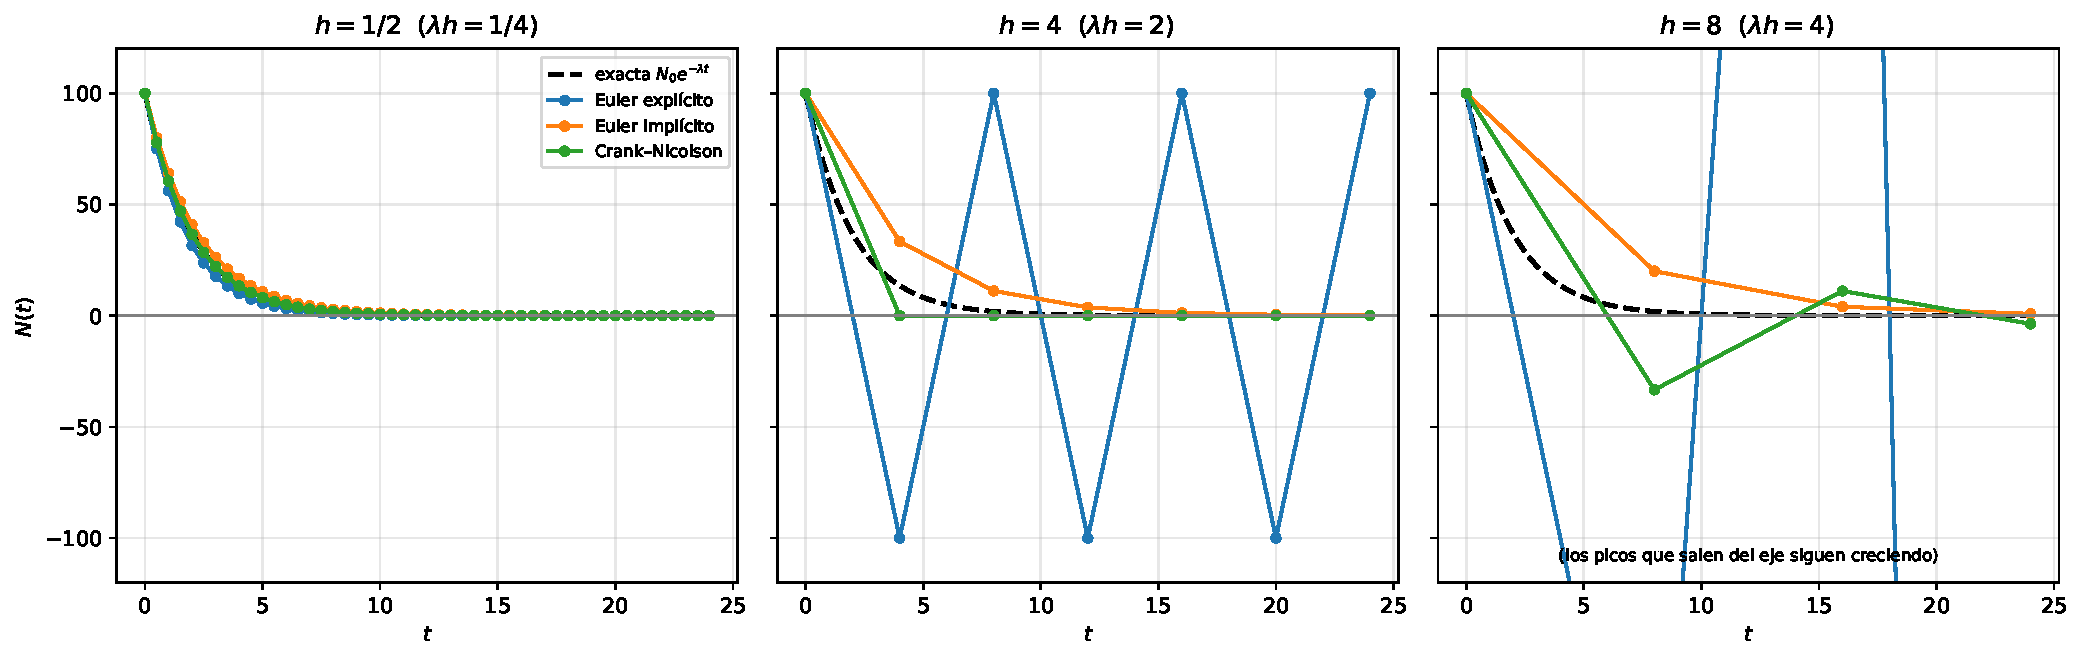
\includegraphics[width=\textwidth]{p1_decaimiento.pdf}
    \caption{Decaimiento real $N(t)$ contra $t$ ($\lambda=\tfrac12$, $N_0=100$)}
\end{figure}

\begin{figure}[htbp]
    \centering
    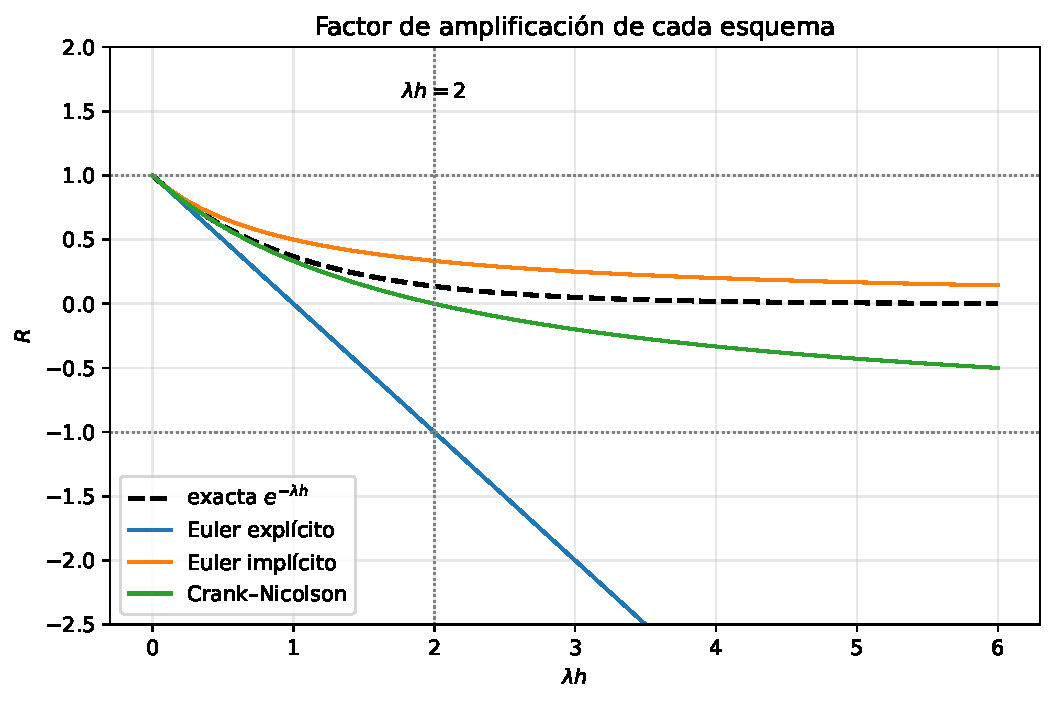
\includegraphics[width=0.8\textwidth]{p1_R_vs_lh.pdf}
    \caption{$R$ contra $\lambda h$}
\end{figure}

\begin{figure}[htbp]
    \centering
    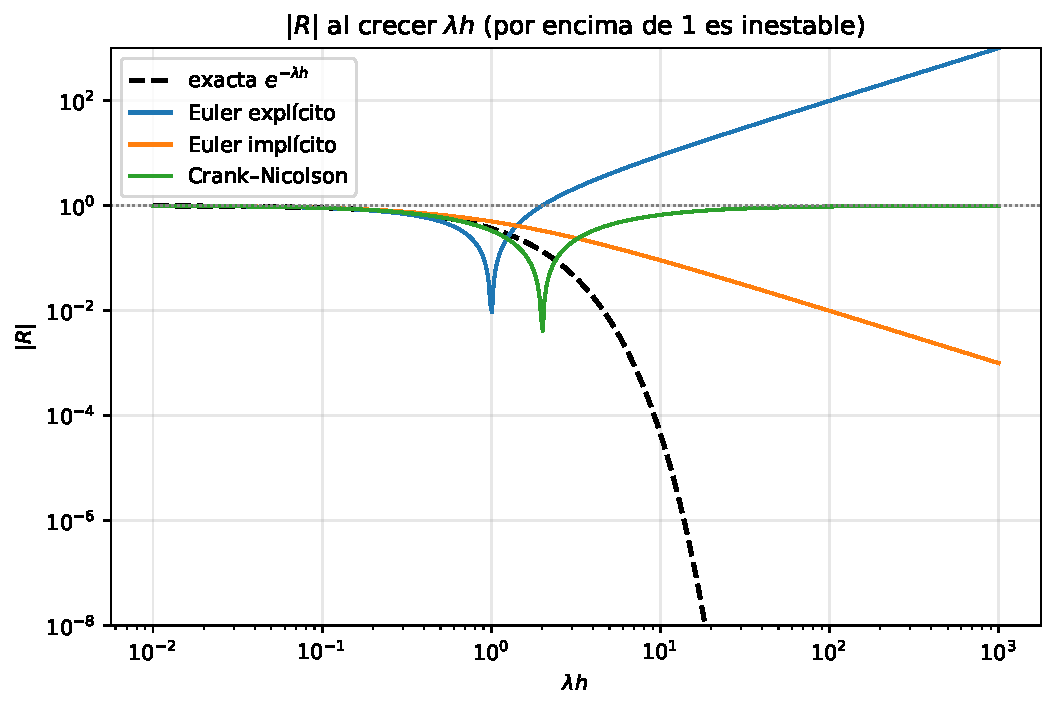
\includegraphics[width=0.8\textwidth]{p1_R_limite.pdf}
    \caption{$|R|$ cuando $\lambda h \to \infty$ (escala logarítmica).}
\end{figure}

Cree un notebook de Python para estudiar el comportamiento el repositorio lo subi a GitHub:
\url{\repoCIN}.

% !TeX root = ../main.tex
\problema{2}{Demostración numérica: CN es de orden 3 local y 2 global}{8}

\begin{enunciado}
	Considere $N' = -\lambda N$ con $\lambda = 1$, $N_0 = 100$.
	\begin{enumerate}[label=(\alph*)]
		\item Demuestre con $z = \lambda h$, que
		$e^{z} - R_{\mathrm{CN}}(z) = -\dfrac{z^3}{12} + \Order{z^4}$,
		$R_{\mathrm{CN}}(z) = \dfrac{1 + z/2}{1 - z/2}$.
		Concluya que el error local es $\dfrac{\lambda^3 h^3}{12} N_n + \Order{h^4}$.
		\item \textbf{Error local.} Complete la tabla con
		$e_{\mathrm{loc}}(\lambda h) = \left| e^{-\lambda h} - R_{\mathrm{CN}}(-\lambda h)\right|$
		(un solo paso desde $t = 0$) y
		$p_{\mathrm{loc}} = \log_2\!\big(e_{\mathrm{loc}}(2h)/e_{\mathrm{loc}}(h)\big)$.
		
		\begin{center}
			\begin{tabular}{cccc}\toprule
				$h$ & $e_{\mathrm{loc}}(h)$ & $e_{\mathrm{loc}}(2h)/e_{\mathrm{loc}}(h)$ & $p_{\mathrm{loc}}$\\\midrule
				0.40 & & --- & --- \\ 0.20 & & & \\ 0.10 & & & \\ 0.05 & & & \\\bottomrule
			\end{tabular}
		\end{center}
		\item \textbf{Error global.} Integre hasta $T = 1$ con $h = \tfrac12, \tfrac14, \tfrac18, \tfrac1{16}$
		y complete $E(h) = |N_{T/h} - e^{-\lambda}|$ y $p_{\mathrm{glob}}$.

		\begin{center}
			\begin{tabular}{cccc}\toprule
				$h$ & $E(h)$ & $E(2h)/E(h)$ & $p_{\mathrm{glob}}$\\\midrule
				1/2 & & --- & --- \\ 1/4 & & & \\ 1/8 & & & \\ 1/16 & & & \\\bottomrule
			\end{tabular}
		\end{center}
		\item Grafique ambos errores en ejes log--log y estime las pendientes. Explique por qué
		$n = T/h$ pasos con error local $\Order{h^3}$ producen un error global $\Order{h^2}$.
	\end{enumerate}
\end{enunciado}

\subsubsection*{Solución}
\[
\ddt{N} = -\lambda\,N(t), \qquad t \in [0, T], \qquad N(0) = N_0 = 100, \qquad \lambda = 1,
\]
con solución exacta
\[
N(t) = N_0\, e^{-\lambda t} = 100\, e^{-t}.
\]


\inciso{a}{Demo}

\paso{1}{Esquema CN}
Es el mismo esquema del Problema 1 (a): mallado $t_n = n h$, colocación de la EDO en $t_{\nmed}$ y primera
diferencia dividida centrada,
\[
\frac{N_{n+1} - N_n}{h} = -\lambda\,\frac{N_n + N_{n+1}}{2}.
\]
parte algebraica
\begin{align*}
	N_{n+1} - N_n &= -\frac{\lambda h}{2}\,N_n - \frac{\lambda h}{2}\,N_{n+1}\\
	N_{n+1} + \frac{\lambda h}{2}\,N_{n+1} &= N_n - \frac{\lambda h}{2}\,N_n\\
	N_{n+1}\left(1 + \frac{\lambda h}{2}\right) &= N_n\left(1 - \frac{\lambda h}{2}\right)\\
	N_{n+1} &= \left(\frac{1 - \frac{\lambda h}{2}}{1 + \frac{\lambda h}{2}}\right) N_n
\end{align*}
Si en $R_{\mathrm{CN}}(z) = \dfrac{1 + z/2}{1 - z/2}$ se pone $z = -\lambda h$:
\[
R_{\mathrm{CN}}(-\lambda h) = \frac{1 + \frac{-\lambda h}{2}}{1 - \frac{-\lambda h}{2}}
= \frac{1 - \frac{\lambda h}{2}}{1 + \frac{\lambda h}{2}},
\]
\[
N_{n+1} = R_{\mathrm{CN}}(-\lambda h)\,N_n .
\]
La exacta es:
\[
N(t_{n+1}) = N_0\, e^{-\lambda (t_n + h)} = e^{-\lambda h}\, N_0\, e^{-\lambda t_n} = e^{-\lambda h}\,N(t_n).
\]
Tenemos que comparar $e^{-\lambda h}$ (exacta) contra $R_{\mathrm{CN}}(-\lambda h)$ 


\paso{2}{Serie de $R_{\mathrm{CN}}(z)$}
serie del denominador:
\[
R_{\mathrm{CN}}(z) = \frac{1 + \frac{z}{2}}{1 - \frac{z}{2}} = \left(1 + \frac{z}{2}\right)\cdot\frac{1}{1 - \frac{z}{2}} .
\]

\textbf{Serie geométrica.} Para $|w| < 1$,
\[
\frac{1}{1 - w} = 1 + w + w^2 + w^3 + \Order{w^4}.
\]
Se comprueba multiplicando por $(1 - w)$:
\begin{align*}
	(1 - w)\left(1 + w + w^2 + w^3\right) &= 1 + w + w^2 + w^3 - w - w^2 - w^3 - w^4\\
	&= 1 - w^4
\end{align*}
como $w$ es pequeño entonces $w^4$ es despreciable $(1 - w)(1 + w + w^2 + w^3) \approx 1$.

\textbf{Con $w = z/2$}
\begin{align*}
	\frac{1}{1 - \frac{z}{2}} &= 1 + \frac{z}{2} + \left(\frac{z}{2}\right)^2 + \left(\frac{z}{2}\right)^3 + \Order{z^4}\\
	&= 1 + \frac{z}{2} + \frac{z^2}{4} + \frac{z^3}{8} + \Order{z^4}
\end{align*}

\textbf{Multiplicar por el numerador.} En $R_{\mathrm{CN}}(z) = \left(1 + \frac{z}{2}\right)\cdot\frac{1}{1 - z/2}$
\begin{align*}
	R_{\mathrm{CN}}(z) &= \left(1 + \frac{z}{2}\right)\left(1 + \frac{z}{2} + \frac{z^2}{4} + \frac{z^3}{8} + \Order{z^4}\right)\\
	&= 1\cdot\left(1 + \frac{z}{2} + \frac{z^2}{4} + \frac{z^3}{8}\right)
	+ \frac{z}{2}\cdot\left(1 + \frac{z}{2} + \frac{z^2}{4} + \frac{z^3}{8}\right) + \Order{z^4}\\
	&= 1 + \frac{z}{2} + \frac{z^2}{4} + \frac{z^3}{8}
	+ \frac{z}{2} + \frac{z^2}{4} + \frac{z^3}{8} + \frac{z^4}{16} + \Order{z^4}\\
	&= 1 + \frac{z}{2} + \frac{z^2}{4} + \frac{z^3}{8}
	+ \frac{z}{2} + \frac{z^2}{4} + \frac{z^3}{8} + \Order{z^4}
\end{align*}
Reacomodando
\begin{align*}
	R_{\mathrm{CN}}(z) &= 1 + \left(\frac12 + \frac12\right) z + \left(\frac14 + \frac14\right) z^2 + \left(\frac18 + \frac18\right) z^3 + \Order{z^4}\\
	&= 1 + z + \frac{2}{4}\,z^2 + \frac{2}{8}\,z^3 + \Order{z^4}\\
	&= 1 + z + \frac{z^2}{2} + \frac{z^3}{4} + \Order{z^4}
\end{align*}
\resultado{R_{\mathrm{CN}}(z) = 1 + z + \frac{z^2}{2} + \frac{z^3}{4} + \Order{z^4}}
\paso{3}{Restar la serie de Taylor de $e^{z}$}
Para comparar $e^{z}$ (exacta) con $R_{\mathrm{CN}}(z)$ potencia por potencia, se escribe $e^{z}$ también como serie.
Por Taylor alrededor de $z = 0$, como todas las derivadas de $e^{z}$ son $e^{z}$ y en $z = 0$ valen $e^{0} = 1$:
\[
e^{z} = 1 + z + \frac{z^2}{2!} + \frac{z^3}{3!} + \Order{z^4} = 1 + z + \frac{z^2}{2} + \frac{z^3}{6} + \Order{z^4}
\]
\begin{align*}
	e^{z} - R_{\mathrm{CN}}(z) &= \left(1 - 1\right) + \left(z - z\right) + \left(\frac{z^2}{2} - \frac{z^2}{2}\right)
	+ \left(\frac16 - \frac14\right) z^3 + \Order{z^4}\\
	&= \left(\frac{2}{12} - \frac{3}{12}\right) z^3 + \Order{z^4}\\
	&= -\frac{z^3}{12} + \Order{z^4}
\end{align*}

\resultado{e^{z} - R_{\mathrm{CN}}(z) = -\frac{z^3}{12} + \Order{z^4}}

\paso{4}{Error local}
El error local es el que se comete en \textbf{un solo paso}
\[
e_{\mathrm{loc},n} = N(t_{n+1}) - N_{n+1}.
\]
Sustituyendo la exacta, CN y el resultado del paso 3 con $z = -\lambda h$:
\begin{align*}
	e_{\mathrm{loc},n} &= e^{-\lambda h}\,N(t_n) - R_{\mathrm{CN}}(-\lambda h)\,N(t_n)\\
	&= \left[e^{-\lambda h} - R_{\mathrm{CN}}(-\lambda h)\right] N(t_n)\\
	&= \left[-\frac{(-\lambda h)^3}{12} + \Order{h^4}\right] N(t_n)\\
	&= \left[-\frac{-\lambda^3 h^3}{12} + \Order{h^4}\right] N(t_n)\\
	&= \frac{\lambda^3 h^3}{12}\,N(t_n) + \Order{h^4}
\end{align*}

\resultado{e_{\mathrm{loc},n} = \frac{\lambda^3 h^3}{12}\,N_n + \Order{h^4}}
Sale positivo, o sea que en cada paso CN se queda un poquito por debajo de la exacta. Es el mismo resultado que salió
para CN en el Problema 1.

\inciso{b}{Error local: tabla y orden observado}


\paso{1}{calculo}
Con $\lambda = 1$ se da un paso desde $t_0 = 0$ donde el valor inicial es exacto. Del inciso (a),
$e_{\mathrm{loc},0} = \left[e^{-\lambda h} - R_{\mathrm{CN}}(-\lambda h)\right] N_0$
\[
e_{\mathrm{loc}}(h) = \frac{|e_{\mathrm{loc},0}|}{N_0} = \left| e^{-\lambda h} - R_{\mathrm{CN}}(-\lambda h) \right|
= \left| e^{-h} - \frac{2 - h}{2 + h} \right| ,
\]
donde $R_{\mathrm{CN}}(-h) = \dfrac{1 - h/2}{1 + h/2}$ se multiplicó arriba y abajo por 2. Con $N_0 = 100$ el error
saldría 100 veces mayor, pero el orden es el mismo.

\paso{2}{Cálculo renglón por renglón}
La resta se hace con todos los decimales de la calculadora, porque $e^{-h}$ y $R_{\mathrm{CN}}$ se parecen mucho y si se
redondean antes se pierden cifras del error.
\begin{align*}
	h = 0.40:&\quad R_{\mathrm{CN}} = \frac{2 - 0.40}{2 + 0.40} = \frac{1.6}{2.4} = \frac23, y
	\qquad e^{-0.40} \\
	&\quad e_{\mathrm{loc}} = e^{-0.40} - \frac23 \approx 3.653379\times10^{-3}\\[6pt]
	h = 0.20:&\quad R_{\mathrm{CN}} = \frac{2 - 0.20}{2 + 0.20} = \frac{1.8}{2.2} = \frac{9}{11} , y
	\qquad e^{-0.20} \\
	&\quad e_{\mathrm{loc}} = e^{-0.20} - \frac{9}{11} \approx 5.489349\times10^{-4}\\[6pt]
	h = 0.10:&\quad R_{\mathrm{CN}} = \frac{2 - 0.10}{2 + 0.10} = \frac{1.9}{2.1} = \frac{19}{21} , y
	\qquad e^{-0.10} \\
	&\quad e_{\mathrm{loc}} = e^{-0.10} - \frac{19}{21} \approx 7.551327\times10^{-5}\\[6pt]
	h = 0.05:&\quad R_{\mathrm{CN}} = \frac{2 - 0.05}{2 + 0.05} = \frac{1.95}{2.05} = \frac{39}{41} , y
	\qquad e^{-0.05} \\
	&\quad e_{\mathrm{loc}} = e^{-0.05} - \frac{39}{41} \approx 9.912306\times10^{-6}
\end{align*}
En todos $e^{-h} > R_{\mathrm{CN}}$que es la info que nos daba el inciso a)
\[
p_{\mathrm{loc}} = \frac{\ln\!\left(\dfrac{e_{\mathrm{loc}}(2h)}{e_{\mathrm{loc}}(h)}\right)}{\ln 2}
\]
\begin{align*}
	h = 0.20:&\quad \frac{e_{\mathrm{loc}}(2h)}{e_{\mathrm{loc}}(h)} = \frac{3.653379\times10^{-3}}{5.489349\times10^{-4}} = 6.655396,
	\qquad p_{\mathrm{loc}} = \frac{1.895428}{0.693147} = 2.734525\\
	h = 0.10:&\quad \frac{e_{\mathrm{loc}}(2h)}{e_{\mathrm{loc}}(h)} = \frac{5.489349\times10^{-4}}{7.551327\times10^{-5}} = 7.269383,
	\qquad p_{\mathrm{loc}} = \frac{1.983671}{0.693147} = 2.861833\\
	h = 0.05:&\quad \frac{e_{\mathrm{loc}}(2h)}{e_{\mathrm{loc}}(h)} = \frac{7.551327\times10^{-5}}{9.912306\times10^{-6}} = 7.618134,
	\qquad p_{\mathrm{loc}} = \frac{2.030531}{0.693147} = 2.929438
\end{align*}
\begin{center}
	\begin{tabular}{cccc}\toprule
		$h$ & $e_{\mathrm{loc}}(h)$ & $e_{\mathrm{loc}}(2h)/e_{\mathrm{loc}}(h)$ & $p_{\mathrm{loc}}$\\\midrule
		0.40 & $3.653379\times10^{-3}$ & ---      & ---      \\
		0.20 & $5.489349\times10^{-4}$ & 6.655396 & 2.734525 \\
		0.10 & $7.551327\times10^{-5}$ & 7.269383 & 2.861833 \\
		0.05 & $9.912306\times10^{-6}$ & 7.618134 & 2.929438 \\\bottomrule
	\end{tabular}
\end{center}

\inciso{c}{Error global en \texorpdfstring{$T = 1$}{T = 1} y orden observado}
\[
N_{n} = R_{\mathrm{CN}}^{\,n}\,N_0, \qquad
R_{\mathrm{CN}} = \frac{1 - \frac{h}{2}}{1 + \frac{h}{2}} = \frac{2 - h}{2 + h}, \qquad n = \frac{T}{h}, \qquad
N(1) = 100\,e^{-1} \approx 36.787944
\]
\[
E(h) = \left| N_{T/h} - 100\,e^{-1} \right|
\]
\begin{align*}
	h = \tfrac12,\ n = 2:&\quad R_{\mathrm{CN}} = \frac{2 - \frac12}{2 + \frac12} = \frac35, \qquad
	N_2 = 100\left(\frac35\right)^2 = 36.0\\
	&\quad E = 100\,e^{-1} - N_2 \approx 7.879441\times10^{-1}\\[6pt]
	h = \tfrac14,\ n = 4:&\quad R_{\mathrm{CN}} = \frac{2 - \frac14}{2 + \frac14} = \frac79, \qquad
	N_4 = 100\left(\frac79\right)^4 \approx 36.595031\\
	&\quad E = 100\,e^{-1} - N_4 \approx 1.929129\times10^{-1}\\[6pt]
	h = \tfrac18,\ n = 8:&\quad R_{\mathrm{CN}} = \frac{2 - \frac18}{2 + \frac18} = \frac{15}{17}, \qquad
	N_8 = 100\left(\frac{15}{17}\right)^8 \approx 36.739962\\
	&\quad E = 100\,e^{-1} - N_8 \approx 4.798223\times10^{-2}\\[6pt]
	h = \tfrac1{16},\ n = 16:&\quad R_{\mathrm{CN}} = \frac{2 - \frac1{16}}{2 + \frac1{16}} = \frac{31}{33}, \qquad
	N_{16} = 100\left(\frac{31}{33}\right)^{16} \approx 36.775964\\
	&\quad E = 100\,e^{-1} - N_{16} \approx 1.198031\times10^{-2}
\end{align*}
\[
p_{\mathrm{glob}} = \frac{\ln\!\left(\dfrac{E(2h)}{E(h)}\right)}{\ln 2}, \qquad \ln 2 \approx 0.693147
\]
\begin{align*}
	h = \tfrac14:&\quad \frac{E(2h)}{E(h)} = \frac{7.879441\times10^{-1}}{1.929129\times10^{-1}} = 4.084456,
	\qquad p_{\mathrm{glob}} = \frac{1.407189}{0.693147} = 2.030144\\
	h = \tfrac18:&\quad \frac{E(2h)}{E(h)} = \frac{1.929129\times10^{-1}}{4.798223\times10^{-2}} = 4.020506,
	\qquad p_{\mathrm{glob}} = \frac{1.391408}{0.693147} = 2.007377\\
	h = \tfrac1{16}:&\quad \frac{E(2h)}{E(h)} = \frac{4.798223\times10^{-2}}{1.198031\times10^{-2}} = 4.005090,
	\qquad p_{\mathrm{glob}} = \frac{1.387566}{0.693147} = 2.001835
\end{align*}
\begin{center}
	\begin{tabular}{ccccc}\toprule
		$h$ & $N_{T/h}$ & $E(h)$ & $E(2h)/E(h)$ & $p_{\mathrm{glob}}$\\\midrule
		1/2  & 36.000000 & $7.879441\times10^{-1}$ & ---      & ---      \\
		1/4  & 36.595031 & $1.929129\times10^{-1}$ & 4.084456 & 2.030144 \\
		1/8  & 36.739962 & $4.798223\times10^{-2}$ & 4.020506 & 2.007377 \\
		1/16 & 36.775964 & $1.198031\times10^{-2}$ & 4.005090 & 2.001835 \\\bottomrule
	\end{tabular}
\end{center}
\resultado{\frac{E(2h)}{E(h)} \to 4 = 2^2, \qquad p_{\mathrm{glob}} \to 2}

\inciso{d}{Gráfica log--log, pendientes y por qué el orden baja de 3 a 2}

\begin{center}
	\begin{tabular}{cccc}\toprule
		\multicolumn{4}{c}{Error local}\\\midrule
		$h$ & $\log_{10} h$ & $e_{\mathrm{loc}}$ & $\log_{10} e_{\mathrm{loc}}$\\\midrule
		0.40 & $-0.397940$ & $3.653379\times10^{-3}$ & $-2.437305$\\
		0.20 & $-0.698970$ & $5.489349\times10^{-4}$ & $-3.260479$\\
		0.10 & $-1.000000$ & $7.551327\times10^{-5}$ & $-4.121977$\\
		0.05 & $-1.301030$ & $9.912306\times10^{-6}$ & $-5.003825$\\\bottomrule
	\end{tabular}
	
	\bigskip
	\begin{tabular}{cccc}\toprule
		\multicolumn{4}{c}{Error global}\\\midrule
		$h$ & $\log_{10} h$ & $E$ & $\log_{10} E$\\\midrule
		1/2  & $-0.301030$ & $7.879441\times10^{-1}$ & $-0.103505$\\
		1/4  & $-0.602060$ & $1.929129\times10^{-1}$ & $-0.714639$\\
		1/8  & $-0.903090$ & $4.798223\times10^{-2}$ & $-1.318920$\\
		1/16 & $-1.204120$ & $1.198031\times10^{-2}$ & $-1.921532$\\\bottomrule
	\end{tabular}
\end{center}

\figurapython{p02_loglog}{Error local y global de CN en ejes log--log }{fig:p02_loglog}{0.6}

Del repositorio de GitHub (\url{\repoCIN})

\[
m = \frac{\Delta \log_{10} E}{\Delta \log_{10} h}
\]
\begin{align*}
	\text{local:}\quad  m &= \frac{-5.003825 - (-2.437305)}{-1.301030 - (-0.397940)}
	= \frac{-2.566520}{-0.903090} = 2.841932\\
	\text{global:}\quad m &= \frac{-1.921532 - (-0.103505)}{-1.204120 - (-0.301030)}
	= \frac{-1.818027}{-0.903090} = 2.013118
\end{align*}

En cada paso se comete un error local $\approx C\,h^3$ y para llegar a $T$ se necesitan $n = T/h$ pasos. Como CN es
estable ($|R| < 1$), los errores no se amplifican, solo se suman:
\begin{align*}
	E &\approx n \cdot C\,h^3\\
	&= \frac{T}{h}\cdot C\,h^3\\
	&= C\,T\,h^2
\end{align*}
\resultado{e_{\mathrm{loc}} = \Order{h^3}, \qquad E = \Order{h^2}}

% !TeX root = ../main.tex
\problema{3}{Decaimiento con fuente}{6}

\begin{enunciado}
	Sea $N' = -\lambda N + S$, con $\lambda = 2$, $S = 4$ (constante), $N_0 = 0$.
	\begin{enumerate}[label=(\alph*)]
		\item Escriba el esquema CN con fuente (promedio de $S$ en $t_n$ y $t_{n+1}$).
		\item Con $h = \frac14$ calcule $N_1$ y $N_2$ y compare con
		$N(t) = \frac{S}{\lambda}\left(1 - e^{-\lambda t}\right)$.
		\item Muestre que $N^* = S/\lambda$ es punto fijo de CN y de Euler implícito.
		\item Calcule el error global en $T = 1$ para $h = \frac12, \frac14, \frac18$ y estime el orden observado.
	\end{enumerate}
\end{enunciado}

% ---------------------------------------------------------------------
\subsubsection*{Solución}
% ---------------------------------------------------------------------
\[
\ddt{N} = \underbrace{-\lambda\,N(t)}_{\text{pérdida}} + \underbrace{S}_{\text{producción}},
\qquad t \in [0, T], \qquad N(0) = N_0 = 0,
\]
con solución exacta
\[
N(t) = \frac{S}{\lambda}\left(1 - e^{-\lambda t}\right) = 2\left(1 - e^{-2t}\right).
\]

% =====================================================================
\inciso{a}{Esquema CN con fuente}
% =====================================================================

\paso{1}{Generación del mallado}
Se divide el intervalo de tiempo $[0, T]$ en pedazos iguales de tamaño $h$:
\[
t_n = n h, \qquad n = 0, 1, 2, \dots
\]

$N(t_n)$ es el valor exacto en el nodo y $N_n$ es la aproximación.

\paso{2}{Colocación de la EDO en $t_{\nmed}$}
$t_{\nmed} = t_n + h/2$:
\[
\left.\ddt{N}\right|_{t_{\nmed}} = -\lambda\, N(t_{\nmed}) + S .
\]

\paso{3}{Sustituir la derivada por la primera diferencia dividida centrada}
se usa Taylor alrededor de $t_{\nmed}$
\[
\left.\ddt{N}\right|_{t_{\nmed}} = \frac{N(t_{n+1}) - N(t_n)}{h} + \Order{h^2}.
\]
El valor en el punto medio, se aproxima con el promedio de los dos nodos de alado
\[
N(t_{\nmed}) = \frac{N(t_n) + N(t_{n+1})}{2} + \Order{h^2},
\]
y la fuente es constante, así que su promedio es ella misma:
\[
\frac{S + S}{2} = S = 4 .
\]
Reescribiendo:
\[
\frac{N(t_{n+1}) - N(t_n)}{h} = -\lambda\,\frac{N(t_n) + N(t_{n+1})}{2} + S + \Order{h^2}.
\]
El $+\Order{h^2}$ es la suma de los errorcitos.
Hacer la aproximacion
\[
\frac{N_{n+1} - N_n}{h} = -\lambda\,\frac{N_n + N_{n+1}}{2} + S .
\]
parte algebraica
\begin{align*}
	N_{n+1} - N_n &= -\frac{\lambda h}{2}\,N_n - \frac{\lambda h}{2}\,N_{n+1} + hS\\
	N_{n+1} + \frac{\lambda h}{2}\,N_{n+1} &= N_n - \frac{\lambda h}{2}\,N_n + hS\\
	N_{n+1}\left(1 + \frac{\lambda h}{2}\right) &= N_n\left(1 - \frac{\lambda h}{2}\right) + hS
\end{align*}
\resultado{N_{n+1} = \underbrace{\left(\frac{1 - \frac{\lambda h}{2}}{1 + \frac{\lambda h}{2}}\right)}_{R}N_n
	+ \frac{hS}{1 + \frac{\lambda h}{2}}}

% =====================================================================
\inciso{b}{\texorpdfstring{$h = \tfrac14$}{h = 1/4}}
% =====================================================================
Con $\lambda = 2$, $S = 4$ y $h = \frac14$:
\[
\frac{\lambda h}{2} = \frac{2\cdot\frac14}{2} = \frac14, \qquad
R = \frac{1 - \frac14}{1 + \frac14} = \frac{3/4}{5/4} = \frac35, \qquad
\frac{hS}{1 + \frac14} = \frac{1}{5/4} = \frac45 .
\]
$N_{n+1} = \frac35\,N_n + \frac45$. inicia con $N_0 = 0$:
\begin{align*}
	n = 0:&\quad N_1 = \tfrac35(0) + \tfrac45 = \tfrac45 = 0.8\\
	n = 1:&\quad N_2 = \tfrac35\left(\tfrac45\right) + \tfrac45 = \tfrac{12}{25} + \tfrac{20}{25} = \tfrac{32}{25} = 1.28
\end{align*}
La solución exacta: con $t_0 = 0$ y paso $h = \frac14$, $t_1 = 0.25$ y $t_2 = 0.5$:
\begin{align*}
	N(0.25) &= 2\left(1 - e^{-1/2}\right) \approx 0.786939\\
	N(0.5)  &= 2\left(1 - e^{-1}\right) \approx 1.264241
\end{align*}
Comparacion
\begin{center}
	\begin{tabular}{cccc}\toprule
		$n$ & CN & exacta & $|N(t_n) - N_n|$\\\midrule
		1 & 0.8  & 0.786939 & 0.013061\\
		2 & 1.28 & 1.264241 & 0.015759\\\bottomrule
	\end{tabular}
\end{center}

CN sobreestima un poco. Pero notamos que el Error$_{N_2}$ $>$ Error$_{N_1}$ porque $N_2$
arrastra el error de $N_1$ mas el error de el.

Se graficaron todos los valores con Python para ver su comportamiento

\begin{center}
	\tablapython{p3_b_todos}
\end{center}

\figurapython{p3_solucion}{Solución exacta, Crank--Nicolson y Euler implícito
	tienden al punto fijo}{fig:p3sol}{0.75}


\inciso{c}{\texorpdfstring{$N^* = S/\lambda$}{N* = S/lambda} es punto fijo de CN y de Euler implícito}

$N^*$ es \textbf{punto fijo} del esquema si, cuando $N_n = N^*$, el esquema devuelve $N_{n+1} = N^*$
La ecuación exacta tiene equilibrio en $N^* = S/\lambda = 4/2 = 2$.

\textbf{Crank--Nicolson.} Si $N_n = S/\lambda$:
\begin{align*}
	N_{n+1}\left(1 + \frac{\lambda h}{2}\right) &= \frac{S}{\lambda}\left(1 - \frac{\lambda h}{2}\right) + hS\\
	&= \frac{S}{\lambda} - \frac{hS}{2} + hS\\
	&= \frac{S}{\lambda} + \frac{hS}{2}\\
	&= \frac{S}{\lambda}\left(1 + \frac{\lambda h}{2}\right)\\
	N_{n+1} &= \frac{S}{\lambda}
\end{align*}

\textbf{Euler implícito.} Se construye con la misma receta, colocando la EDO en $t_{n+1}$ y se usa la primera
diferencia dividida regresiva:
\begin{align*}
	\frac{N_{n+1} - N_n}{h} &= -\lambda N_{n+1} + S\\
	N_{n+1} - N_n &= -\lambda h\,N_{n+1} + hS\\
	N_{n+1}\left(1 + \lambda h\right) &= N_n + hS
\end{align*}
Con $N_n = S/\lambda$:
\begin{align*}
	N_{n+1}\left(1 + \lambda h\right) &= \frac{S}{\lambda} + hS\\
	&= \frac{S}{\lambda}\left(1 + \lambda h\right)\\
	N_{n+1} &= \frac{S}{\lambda}
\end{align*}
\resultado{N^* = \frac{S}{\lambda} = 2 \text{ es punto fijo de CN y de Euler implícito}}


\inciso{d}{Error global en \texorpdfstring{$T = 1$}{T = 1} y orden observado}

Del inciso (a), con $\lambda = 2$ y $S = 4$:
\[
N_{n+1} = R\,N_n + c, \qquad
R = \frac{1 - \frac{\lambda h}{2}}{1 + \frac{\lambda h}{2}} = \frac{1 - h}{1 + h}, \qquad
c = \frac{hS}{1 + \frac{\lambda h}{2}} = \frac{4h}{1 + h}
\]
Solución exacta en $T = 1$ y error global:
\[
N(1) = 2\left(1 - e^{-2}\right) \qquad E(h) = \left|N_{T/h} - N(1)\right|
\]

$h = \tfrac12$, $n = 2$ 
\begin{align*}
	R &= \frac{1 - \frac12}{1 + \frac12} = \frac{\frac12}{\frac32} = \frac13\\
	c &= \frac{4\cdot\frac12}{1 + \frac12} = \frac{2}{\frac32} = \frac43\\
	N_1 &= \tfrac13(0) + \tfrac43 = \tfrac43 \\
	N_2 &= \tfrac13\left(\tfrac43\right) + \tfrac43 = \tfrac49 + \tfrac{12}{9} = \tfrac{16}{9} \\
	E &= \tfrac{16}{9} - 1.729329 \approx 4.844834\times10^{-2}
\end{align*}

$h = \tfrac14$, $n = 4$ 
\begin{align*}
	R &= \frac{1 - \frac14}{1 + \frac14} = \frac{\frac34}{\frac54} = \frac35\\
	c &= \frac{4\cdot\frac14}{1 + \frac14} = \frac{1}{\frac54} = \frac45\\
	N_1 &= \tfrac35(0) + \tfrac45 = 0.8\\
	N_2 &= \tfrac35(0.8) + 0.8 = 1.28\\
	N_3 &= \tfrac35(1.28) + 0.8 = 1.568\\
	N_4 &= \tfrac35(1.568) + 0.8 = 1.7408\\
	E &= 1.740800 - 1.729329 \approx 1.147057\times10^{-2}
\end{align*}

$h = \tfrac18$, $n = 8$
\begin{align*}
	R &= \frac{1 - \frac18}{1 + \frac18} = \frac{\frac78}{\frac98} = \frac79\\
	c &= \frac{4\cdot\frac18}{1 + \frac18} = \frac{\frac12}{\frac98} = \frac49\\
	N_1 &= \tfrac79(0) + \tfrac49 \approx 0.444444\\
	N_2 &= \tfrac79(0.444444) + \tfrac49 \approx 0.790123\\
	N_3 &= \tfrac79(0.790123) + \tfrac49 \approx 1.058985\\
	N_4 &= \tfrac79(1.058985) + \tfrac49 \approx 1.268099\\
	N_5 &= \tfrac79(1.268099) + \tfrac49 \approx 1.430744\\
	N_6 &= \tfrac79(1.430744) + \tfrac49 \approx 1.557245\\
	N_7 &= \tfrac79(1.557245) + \tfrac49 \approx 1.655635\\
	N_8 &= \tfrac79(1.655635) + \tfrac49 \approx 1.732161\\
	E &= 1.732161 - 1.729329 \approx 2.831304\times10^{-3}
\end{align*}

\textbf{Orden}
\[
p_{\mathrm{glob}} = \frac{\ln\!\left(\dfrac{E(2h)}{E(h)}\right)}{\ln 2}, \qquad \ln 2 
\]
\begin{align*}
	h = \tfrac14:&\quad \frac{E(2h)}{E(h)} = \frac{4.844834\times10^{-2}}{1.147057\times10^{-2}} = 4.223710\\
	&\quad p_{\mathrm{glob}} = \frac{\ln(4.223710)}{\ln 2} = \frac{1.440714}{0.693147} = 2.078511\\[6pt]
	h = \tfrac18:&\quad \frac{E(2h)}{E(h)} = \frac{1.147057\times10^{-2}}{2.831304\times10^{-3}} = 4.051337\\
	&\quad p_{\mathrm{glob}} = \frac{\ln(4.051337)}{\ln 2} = \frac{1.399047}{0.693147} = 2.018398
\end{align*}
\begin{center}
	\begin{tabular}{ccccc}\toprule
		$h$ & $N_{T/h}$ & $E(h)$ & $E(2h)/E(h)$ & $p_{\mathrm{glob}}$\\\midrule
		1/2 & 1.777778 & $4.844834\times10^{-2}$ & ---      & ---      \\
		1/4 & 1.740800 & $1.147057\times10^{-2}$ & 4.223710 & 2.078511 \\
		1/8 & 1.732161 & $2.831304\times10^{-3}$ & 4.051337 & 2.018398 \\\bottomrule
	\end{tabular}
\end{center}


\parte{II}{Difusión en estado estacionario}{20}

\problema{4}{Difusión 1D con condiciones de Dirichlet}{8}

\begin{enunciado}
	Resuelva $-D\varphi'' + \Sigma_a \varphi = S$ en $0 < x < L$, con $\varphi(0) = \varphi(L) = 0$,
	$L = 10$, $D = 1$, $\Sigma_a = \tfrac12$, $S = 1$ y $h = 2$ (cuatro nodos interiores).
	
	\begin{center}
		\begin{tikzpicture}[x=1.6cm]
			\draw[thick] (0,0) -- (5,0);
			\foreach \i in {0,...,5} {
				\fill (\i,0) circle (2pt);
				\node[below=3pt] at (\i,0) {$x_{\i}$};
			}
			\node[above=3pt] at (0,0) {$\varphi_0 = 0$};
			\node[above=3pt] at (5,0) {$\varphi_5 = 0$};
			\draw[<->] (2,0.45) -- node[above] {$h$} (3,0.45);
		\end{tikzpicture}
	\end{center}
	
	\begin{enumerate}[label=(\alph*)]
		\item Deduzca la ecuación discreta del nodo interior $i$ y su error de truncamiento.
		\item Escriba el sistema $\mat{A}\vect{\varphi} = \vect{b}$ y verifique que $\mat{A}$ es simétrica definida positiva.
		\item Obtenga la factorización de Gauss $\mat{A} = \mat{L}\mat{U}$.
		\item Obtenga la factorización triple $\mat{A} = \mat{L}\mat{D}\mat{L}^T$ y compare con (c).
		\item Obtenga la factorización de Cholesky $\mat{A} = \mat{G}\mat{G}^T$.
		\item Resuelva el sistema con la factorización de su elección y verifique con la simetría del problema.
		\item Compare el costo de resolver con matriz densa ($\Order{n^3}$) y con matriz tridiagonal.
	\end{enumerate}
\end{enunciado}

% ---------------------------------------------------------------------
\subsubsection*{Solución}
% ---------------------------------------------------------------------

La ecuación es de difusión con absorción y fuente uniforme:
\[
\underbrace{-D\,\frac{\dd^2\varphi}{\dd x^2}}_{\text{fugas}}
+ \underbrace{\Sigma_a\,\varphi}_{\text{absorción}}
= \underbrace{S}_{\text{fuente}},
\qquad x \in [0, L], \qquad \varphi(0) = \varphi(L) = 0,
\]
con $L = 10$, $D = 1$, $\Sigma_a = \tfrac12$, $S = 1$ y $h = 2$.

% =====================================================================
\inciso{a}{Ecuación discreta del nodo interior y error de truncamiento}
% =====================================================================

\paso{1}{Generación del mallado}
Se divide el dominio $[0, L]$ en $I$ pedazos iguales:
\[
h = \frac{L - 0}{I} \;\Longrightarrow\; I = \frac{L}{h} = \frac{10}{2} = 5,
\qquad x_i = 0 + i\,h = 2i, \qquad i = 0, 1, \dots, 5,
\]
es decir,
\[
x_0 = 0, \quad x_1 = 2, \quad x_2 = 4, \quad x_3 = 6, \quad x_4 = 8, \quad x_5 = 10 .
\]
En $x_0$ y $x_5$ el valor ya se conoce por las condiciones de frontera, $\varphi_0 = \varphi_5 = 0$,
así que quedan $I - 1 = 4$ incógnitas: $\varphi_1, \varphi_2, \varphi_3, \varphi_4$.

Colocación de la EDO en $x = x_i$
\[
-D\,\varphi''(x_i) + \Sigma_a\,\varphi(x_i) = S, \qquad i = 1, 2, 3, 4 .
\]

Cambio de la segunda derivada por la segunda diferencia dividida centrada
Con Taylor alrededor de $x_i$ 
\begin{align*}
	\varphi(x_i + h) &= \varphi + h\,\varphi' + \frac{h^2}{2}\varphi'' + \frac{h^3}{6}\varphi'''
	+ \frac{h^4}{24}\varphi^{(4)} + \frac{h^5}{120}\varphi^{(5)} + \Order{h^6}\\
	\varphi(x_i - h) &= \varphi - h\,\varphi' + \frac{h^2}{2}\varphi'' - \frac{h^3}{6}\varphi'''
	+ \frac{h^4}{24}\varphi^{(4)} - \frac{h^5}{120}\varphi^{(5)} + \Order{h^6}
\end{align*}
Al sumar los terminos de orden impar se cancelan
\begin{align*}
	\varphi(x_i + h) &= \varphi + \bcancel{h\,\varphi'} + \frac{h^2}{2}\varphi''
	+ \bcancel{\frac{h^3}{6}\varphi'''} + \frac{h^4}{24}\varphi^{(4)}
	+ \bcancel{\frac{h^5}{120}\varphi^{(5)}} + \Order{h^6}\\
	\varphi(x_i - h) &= \varphi - \bcancel{h\,\varphi'} + \frac{h^2}{2}\varphi''
	- \bcancel{\frac{h^3}{6}\varphi'''} + \frac{h^4}{24}\varphi^{(4)}
	- \bcancel{\frac{h^5}{120}\varphi^{(5)}} + \Order{h^6}
\end{align*}
y los pares se duplican
\[
\varphi(x_{i+1}) + \varphi(x_{i-1})
= 2\varphi(x_i) + h^2\varphi''(x_i) + \frac{h^4}{12}\varphi^{(4)}(x_i) + \Order{h^6}.
\]
Reacomodando
\[
\varphi(x_{i+1}) - 2\varphi(x_i) + \varphi(x_{i-1})
= h^2\varphi''(x_i) + \frac{h^4}{12}\varphi^{(4)}(x_i) + \Order{h^6},
\]
se divide entre $h^2$ $\left(\frac{h^4}{h^2} = h^2,\ \frac{h^6}{h^2} = h^4\right)$:
\[
\frac{\varphi(x_{i+1}) - 2\varphi(x_i) + \varphi(x_{i-1})}{h^2}
= \varphi''(x_i) + \frac{h^2}{12}\varphi^{(4)}(x_i) + \Order{h^4},
\]
y se despeja la segunda derivada:
\begin{align*}
	\varphi''(x_i)
	&= \frac{\varphi(x_{i+1}) - 2\varphi(x_i) + \varphi(x_{i-1})}{h^2} - \frac{h^2}{12}\varphi^{(4)}(x_i) + \Order{h^4}\\
	&= \frac{\varphi(x_{i+1}) - 2\varphi(x_i) + \varphi(x_{i-1})}{h^2} + \Order{h^2}.
\end{align*}

Sustitución en la EDO
Se quita el $\Order{h^2}$ y se introduce en la EDO
\[
-D\,\frac{\varphi_{i+1} - 2\varphi_i + \varphi_{i-1}}{h^2} + \Sigma_a\,\varphi_i = S .
\]
Se reparte el $-D/h^2$
\[
-\frac{D}{h^2}\,\varphi_{i+1} + \frac{2D}{h^2}\,\varphi_i - \frac{D}{h^2}\,\varphi_{i-1} + \Sigma_a\,\varphi_i = S
\]
agrupando
\[
-\frac{D}{h^2}\,\varphi_{i-1} + \left(\frac{2D}{h^2} + \Sigma_a\right)\varphi_i - \frac{D}{h^2}\,\varphi_{i+1} = S
\]

Multiplicación por $h^2$

\[
-D\,\varphi_{i-1} + \left(2D + \Sigma_a h^2\right)\varphi_i - D\,\varphi_{i+1} = S\,h^2 
\]
Con los datos:
\[
D = 1, \qquad
2D + \Sigma_a h^2 = 2(1) + \tfrac12(2)^2 = 2 + 2 = 4, \qquad
S\,h^2 = (1)(2)^2 = 4
\]
\resultado{-\varphi_{i-1} + 4\varphi_i - \varphi_{i+1} = 4}


El error de truncamiento $\tau_i$ es lo que sobra al meter la solución exacta $\varphi(x)$ en la ecuación discreta sin multiplicar por $h^2$, pasando $S$ restando:
\[
\tau_i = -D\,\frac{\varphi(x_{i+1}) - 2\varphi(x_i) + \varphi(x_{i-1})}{h^2} + \Sigma_a\,\varphi(x_i) - S .
\]
Por Taylor, el cociente es
\[
\frac{\varphi(x_{i+1}) - 2\varphi(x_i) + \varphi(x_{i-1})}{h^2}
= \varphi''(x_i) + \frac{h^2}{12}\varphi^{(4)}(x_i) + \Order{h^4},
\]
y al sustituirlo se agrupan los términos de la EDO:
\begin{align*}
	\tau_i
	&= -D\,\varphi''(x_i) - \frac{D\,h^2}{12}\varphi^{(4)}(x_i) + \Order{h^4} + \Sigma_a\,\varphi(x_i) - S\\
	&= \underbrace{\Big[-D\,\varphi''(x_i) + \Sigma_a\,\varphi(x_i) - S\Big]}_{0}
	- \frac{D\,h^2}{12}\varphi^{(4)}(x_i) + \Order{h^4}
\end{align*}
El corchete vale $0$ porque la solución exacta cumple la EDO para $x_i$: $-D\,\varphi''(x_i) + \Sigma_a\,\varphi(x_i) = S$
\resultado{\tau_i = -\frac{D\,h^2}{12}\,\varphi^{(4)}(x_i) + \Order{h^4} = \Order{h^2}}
Con $D = 1$ y $h = 2$: $\tau_i = -\frac{(1)(2)^2}{12}\,\varphi^{(4)}(x_i) + \Order{h^4} = -\frac13\,\varphi^{(4)}(x_i) + \Order{h^4}$
% =====================================================================
\inciso{b}{\texorpdfstring{Sistema $\mat{A}\vect{\varphi} = \vect{b}$ y $\mat{A}$ simétrica definida positiva}{Sistema A phi = b y A simétrica definida positiva}}
% =====================================================================

Ecuación discreta
\[
-\varphi_{i-1} + 4\varphi_i - \varphi_{i+1} = 4, \qquad i = 1, 2, 3, 4,
\]
con las fronteras $\varphi_0 = \varphi(0) = 0$ y $\varphi_5 = \varphi(10) = 0$.

Sustitución nodo por nodo
Se sustituye $i = 1, 2, 3, 4$ en la fórmula general, en el mismo orden de términos:
\begin{align*}
	i = 1:&\quad -\underbrace{\varphi_0}_{0} + 4\varphi_1 - \varphi_2 = 4
	&&\Longrightarrow\quad 4\varphi_1 - \varphi_2 = 4\\
	i = 2:&\quad -\varphi_1 + 4\varphi_2 - \varphi_3 = 4
	&&\\
	i = 3:&\quad -\varphi_2 + 4\varphi_3 - \varphi_4 = 4
	&&\\
	i = 4:&\quad -\varphi_3 + 4\varphi_4 - \underbrace{\varphi_5}_{0} = 4
	&&\Longrightarrow\quad -\varphi_3 + 4\varphi_4 = 4
\end{align*}

Foma matricial

Sistema de ecuacionbes
\begin{align*}
	\text{Nodo 1:}&\quad \phantom{-}4\varphi_1 - \phantom{4}\varphi_2 + 0\,\varphi_3 + 0\,\varphi_4 = 4\\
	\text{Nodo 2:}&\quad -\varphi_1 + 4\varphi_2 - \phantom{4}\varphi_3 + 0\,\varphi_4 = 4\\
	\text{Nodo 3:}&\quad \phantom{-}0\,\varphi_1 - \phantom{4}\varphi_2 + 4\varphi_3 - \phantom{4}\varphi_4 = 4\\
	\text{Nodo 4:}&\quad \phantom{-}0\,\varphi_1 + 0\,\varphi_2 - \phantom{4}\varphi_3 + 4\varphi_4 = 4
\end{align*}
Los coeficientes de cada renglón forman un renglón de $\mat{A}$ y los lados derechos forman $\vect{b}$:
\resultado{
	\underbrace{\begin{pmatrix} 4 & -1 & 0 & 0\\ -1 & 4 & -1 & 0\\ 0 & -1 & 4 & -1\\ 0 & 0 & -1 & 4 \end{pmatrix}}_{\mat{A}}
	\underbrace{\begin{pmatrix} \varphi_1\\ \varphi_2\\ \varphi_3\\ \varphi_4 \end{pmatrix}}_{\vect{\varphi}}
	=
	\underbrace{\begin{pmatrix} 4\\ 4\\ 4\\ 4 \end{pmatrix}}_{\vect{b}}
}

Simétrica y definida positiva

Simetría: los renglones de $\mat{A}^T$ son las columnas de $\mat{A}$,
\[
\mat{A}^T =
\begin{pmatrix} 4 & -1 & 0 & 0\\ -1 & 4 & -1 & 0\\ 0 & -1 & 4 & -1\\ 0 & 0 & -1 & 4 \end{pmatrix}
= \mat{A}.
\]

\inciso{c}{\texorpdfstring{Factorización de Gauss $\mat{A} = \mat{L}\mat{U}$}{Factorización de Gauss A = LU}}

$\mat{L}\mat{U} = \mat{A}$
Cada elemento $(i,j)$ de $\mat{L}\mat{U}$ es el renglón $i$ de $\mat{L}$ por la columna $j$ de $\mat{U}$:
\begin{align*}
	\text{Renglón 1:}&\quad (1)(4) = 4, \qquad (1)(-1) = -1, \qquad (1)(0) = 0, \qquad (1)(0) = 0\\
	\text{Renglón 2:}&\quad \left(-\tfrac14\right)(4) = -1\\
	&\quad \left(-\tfrac14\right)(-1) + (1)\left(\tfrac{15}{4}\right) = \tfrac14 + \tfrac{15}{4} = \tfrac{16}{4} = 4\\
	&\quad \left(-\tfrac14\right)(0) + (1)(-1) = -1, \qquad \left(-\tfrac14\right)(0) + (1)(0) = 0\\
	\text{Renglón 3:}&\quad (0)(4) = 0\\
	&\quad \left(-\tfrac{4}{15}\right)\left(\tfrac{15}{4}\right) = -1\\
	&\quad \left(-\tfrac{4}{15}\right)(-1) + (1)\left(\tfrac{56}{15}\right) = \tfrac{4}{15} + \tfrac{56}{15} = \tfrac{60}{15} = 4\\
	&\quad \left(-\tfrac{4}{15}\right)(0) + (1)(-1) = -1\\
	\text{Renglón 4:}&\quad (0)(4) = 0, \qquad (0)(-1) = 0\\
	&\quad \left(-\tfrac{15}{56}\right)\left(\tfrac{56}{15}\right) = -1\\
	&\quad \left(-\tfrac{15}{56}\right)(-1) + (1)\left(\tfrac{209}{56}\right) = \tfrac{15}{56} + \tfrac{209}{56} = \tfrac{224}{56} = 4
\end{align*}
Con esos valores
\[
\mat{L}\mat{U} =
\begin{pmatrix} 4 & -1 & 0 & 0\\ -1 & 4 & -1 & 0\\ 0 & -1 & 4 & -1\\ 0 & 0 & -1 & 4 \end{pmatrix} = \mat{A}
\]
$\mat{U} = \mat{A}$. La matriz $\mat{L}$ es triangular inferior: unos en la diagonal, ceros arriba y cada multiplicador $l_{ik}$ debajo de la diagonal, en la posición $(i,k)$ donde se hizo el cero:
\resultado{
	\mat{L} = \begin{pmatrix} 1 & 0 & 0 & 0\\[3pt] -\frac14 & 1 & 0 & 0\\[3pt] 0 & -\frac{4}{15} & 1 & 0\\[3pt] 0 & 0 & -\frac{15}{56} & 1 \end{pmatrix},
	\qquad
	\mat{U} = \begin{pmatrix} 4 & -1 & 0 & 0\\[3pt] 0 & \frac{15}{4} & -1 & 0\\[3pt] 0 & 0 & \frac{56}{15} & -1\\[3pt] 0 & 0 & 0 & \frac{209}{56} \end{pmatrix}
}


\inciso{d}{\texorpdfstring{Factorización triple $\mat{A} = \mat{L}\mat{D}\mat{L}^T$}{Factorización triple A = LDLT}}



Columna 1
\begin{align*}
	d_1 &= a_{11} = 4\\
	l_{21} &= \frac{a_{21}}{d_1} = \frac{-1}{4} = -\frac14, \qquad
	l_{31} = \frac{a_{31}}{d_1} = \frac{0}{4} = 0, \qquad
	l_{41} = \frac{a_{41}}{d_1} = \frac{0}{4} = 0
\end{align*}

Columna 2
\begin{align*}
	d_2 &= a_{22} - l_{21}^2\,d_1 = 4 - \left(-\tfrac14\right)^2(4) = 4 - \tfrac{1}{16}(4) = 4 - \tfrac14 = \tfrac{15}{4}\\
	l_{32} &= \frac{a_{32} - l_{31}\,d_1\,l_{21}}{d_2} = \frac{-1 - (0)(4)\left(-\frac14\right)}{\frac{15}{4}} = \frac{-1}{\frac{15}{4}} = -\frac{4}{15}\\
	l_{42} &= \frac{a_{42} - l_{41}\,d_1\,l_{21}}{d_2} = \frac{0 - (0)(4)\left(-\frac14\right)}{\frac{15}{4}} = 0
\end{align*}

Columna 3
\begin{align*}
	d_3 &= a_{33} - l_{31}^2\,d_1 - l_{32}^2\,d_2
	= 4 - (0)^2(4) - \left(-\tfrac{4}{15}\right)^2\left(\tfrac{15}{4}\right)\\
	&= 4 - \tfrac{16}{225}\cdot\tfrac{15}{4} = 4 - \tfrac{16\cdot 15}{225\cdot 4} = 4 - \tfrac{240}{900} = 4 - \tfrac{4}{15} = \tfrac{60 - 4}{15} = \tfrac{56}{15}\\
	l_{43} &= \frac{a_{43} - l_{41}\,d_1\,l_{31} - l_{42}\,d_2\,l_{32}}{d_3}
	= \frac{-1 - 0 - 0}{\frac{56}{15}} = -\frac{15}{56}
\end{align*}

Columna 4
\begin{align*}
	d_4 &= a_{44} - l_{41}^2\,d_1 - l_{42}^2\,d_2 - l_{43}^2\,d_3
	= 4 - 0 - 0 - \left(-\tfrac{15}{56}\right)^2\left(\tfrac{56}{15}\right)\\
	&= 4 - \tfrac{15\cdot 15}{56\cdot 56}\cdot\tfrac{56}{15} = 4 - \tfrac{15}{56} = \tfrac{224 - 15}{56} = \tfrac{209}{56}
\end{align*}
\resultado{
	\mat{A} =
	\underbrace{\begin{pmatrix} 1 & 0 & 0 & 0\\[3pt] -\frac14 & 1 & 0 & 0\\[3pt] 0 & -\frac{4}{15} & 1 & 0\\[3pt] 0 & 0 & -\frac{15}{56} & 1 \end{pmatrix}}_{\mat{L}}
	\underbrace{\begin{pmatrix} 4 & 0 & 0 & 0\\[3pt] 0 & \frac{15}{4} & 0 & 0\\[3pt] 0 & 0 & \frac{56}{15} & 0\\[3pt] 0 & 0 & 0 & \frac{209}{56} \end{pmatrix}}_{\mat{D}}
	\underbrace{\begin{pmatrix} 1 & -\frac14 & 0 & 0\\[3pt] 0 & 1 & -\frac{4}{15} & 0\\[3pt] 0 & 0 & 1 & -\frac{15}{56}\\[3pt] 0 & 0 & 0 & 1 \end{pmatrix}}_{\mat{L}^T}
}

\inciso{e}{\texorpdfstring{Factorización de Cholesky $\mat{A} = \mat{G}\mat{G}^T$}{Factorización de Cholesky A = GGT}}


Columna 1
\begin{align*}
	g_{11} &= \sqrt{a_{11}} = \sqrt4 = 2\\
	g_{21} &= \frac{a_{21}}{g_{11}} = \frac{-1}{2} = -\frac12, \qquad
	g_{31} = \frac{a_{31}}{g_{11}} = \frac{0}{2} = 0, \qquad
	g_{41} = \frac{a_{41}}{g_{11}} = \frac{0}{2} = 0
\end{align*}

Columna 2
\begin{align*}
	g_{22} &= \sqrt{a_{22} - g_{21}^2} = \sqrt{4 - \left(-\tfrac12\right)^2} = \sqrt{4 - \tfrac14}
	= \sqrt{\tfrac{15}{4}} = \frac{\sqrt{15}}{2} \approx 1.936492\\
	g_{32} &= \frac{a_{32} - g_{31}\,g_{21}}{g_{22}} = \frac{-1 - (0)\left(-\frac12\right)}{\frac{\sqrt{15}}{2}}
	= -\frac{2}{\sqrt{15}} = -\frac{2\sqrt{15}}{15} \approx -0.516398\\
	g_{42} &= \frac{a_{42} - g_{41}\,g_{21}}{g_{22}} = \frac{0 - (0)\left(-\frac12\right)}{\frac{\sqrt{15}}{2}} = 0
\end{align*}

Columna 3
Con $g_{32}^2 = \left(-\frac{2}{\sqrt{15}}\right)^2 = \frac{4}{15}$:
\begin{align*}
	g_{33} &= \sqrt{a_{33} - g_{31}^2 - g_{32}^2} = \sqrt{4 - 0 - \tfrac{4}{15}} = \sqrt{\tfrac{60 - 4}{15}} = \sqrt{\tfrac{56}{15}}\\
	&= \frac{\sqrt{56\cdot 15}}{15} = \frac{\sqrt{840}}{15} = \frac{\sqrt{4\cdot 210}}{15} = \frac{2\sqrt{210}}{15} \approx 1.932184\\
	g_{43} &= \frac{a_{43} - g_{41}\,g_{31} - g_{42}\,g_{32}}{g_{33}} = \frac{-1 - 0 - 0}{\sqrt{\frac{56}{15}}}
	= -\sqrt{\tfrac{15}{56}}\\
	&= -\frac{\sqrt{15\cdot 56}}{56} = -\frac{\sqrt{840}}{56} = -\frac{2\sqrt{210}}{56} = -\frac{\sqrt{210}}{28} \approx -0.517549
\end{align*}

Columna 4
Con $g_{43}^2 = \frac{15}{56}$:
\begin{align*}
	g_{44} &= \sqrt{a_{44} - g_{41}^2 - g_{42}^2 - g_{43}^2} = \sqrt{4 - 0 - 0 - \tfrac{15}{56}} = \sqrt{\tfrac{224 - 15}{56}} = \sqrt{\tfrac{209}{56}}\\
	&= \frac{\sqrt{209\cdot 56}}{56} = \frac{\sqrt{11704}}{56} = \frac{\sqrt{4\cdot 2926}}{56} = \frac{2\sqrt{2926}}{56} = \frac{\sqrt{2926}}{28} \approx 1.931875
\end{align*}
\resultado{
	\mat{G} =
	\begin{pmatrix}
		2 & 0 & 0 & 0\\[3pt]
		-\frac12 & \frac{\sqrt{15}}{2} & 0 & 0\\[3pt]
		0 & -\frac{2\sqrt{15}}{15} & \frac{2\sqrt{210}}{15} & 0\\[3pt]
		0 & 0 & -\frac{\sqrt{210}}{28} & \frac{\sqrt{2926}}{28}
	\end{pmatrix}
}

\inciso{f}{Solución del sistema y verificación con la simetría}

\paso{1}{Elección de la factorización}
Se usa la factorización triple porque $\mat{A}$ es simétrica y solo necesito "almacenar" $\mat{L}$ y $\mat{D}$
\[
\mat{L}\mat{D}\mat{L}^T\vect{\varphi}= \vect{b},
\]
y se resuelve en tres etapas: (i) $\mat{L}\vect{z} = \vect{b}$, (ii) $\mat{D}\vect{y} = \vect{z}$,
(iii) $\mat{L}^T\vect{\varphi} = \vect{y}$.

\paso{2}{Sustitución hacia adelante, $\mat{L}\vect{z} = \vect{b}$}
\[
\begin{pmatrix} 1 & 0 & 0 & 0\\[3pt] -\frac14 & 1 & 0 & 0\\[3pt] 0 & -\frac{4}{15} & 1 & 0\\[3pt] 0 & 0 & -\frac{15}{56} & 1 \end{pmatrix}
\begin{pmatrix} z_1\\ z_2\\ z_3\\ z_4 \end{pmatrix}
= \begin{pmatrix} 4\\ 4\\ 4\\ 4 \end{pmatrix}
\]
Renglón por renglón:
\[
z_1 = b_1, \qquad l_{21}z_1 + z_2 = b_2, \qquad l_{32}z_2 + z_3 = b_3, \qquad l_{43}z_3 + z_4 = b_4,
\]
$z_1 = b_1$ y $z_i = b_i - l_{i,i-1}\,z_{i-1}$:
\begin{align*}
	z_1 &= b_1 = 4\\
	z_2 &= b_2 - l_{21}\,z_1 = 4 - \left(-\tfrac14\right)(4) = 4 + 1 = 5\\
	z_3 &= b_3 - l_{32}\,z_2 = 4 - \left(-\tfrac{4}{15}\right)(5) = 4 + \tfrac{20}{15} = 4 + \tfrac43 = \tfrac{12 + 4}{3} = \tfrac{16}{3}\\
	z_4 &= b_4 - l_{43}\,z_3 = 4 - \left(-\tfrac{15}{56}\right)\left(\tfrac{16}{3}\right) = 4 + \tfrac{240}{168} = 4 + \tfrac{10}{7} = \tfrac{28 + 10}{7} = \tfrac{38}{7}
\end{align*}


\paso{3}{$\mat{D}\vect{y} = \vect{z}$}
\[
\begin{pmatrix} 4 & 0 & 0 & 0\\[3pt] 0 & \frac{15}{4} & 0 & 0\\[3pt] 0 & 0 & \frac{56}{15} & 0\\[3pt] 0 & 0 & 0 & \frac{209}{56} \end{pmatrix}
\begin{pmatrix} y_1\\ y_2\\ y_3\\ y_4 \end{pmatrix}
= \begin{pmatrix} 4\\[3pt] 5\\[3pt] \frac{16}{3}\\[3pt] \frac{38}{7} \end{pmatrix}
\]

\begin{align*}
	y_1 &= \frac{z_1}{d_1} = \frac{4}{4} = 1\\
	y_2 &= \frac{z_2}{d_2} = \frac{5}{\frac{15}{4}} = 5\cdot\frac{4}{15} = \frac{20}{15} = \frac43\\
	y_3 &= \frac{z_3}{d_3} = \frac{\frac{16}{3}}{\frac{56}{15}} = \frac{16}{3}\cdot\frac{15}{56} = \frac{240}{168} = \frac{10}{7}\\
	y_4 &= \frac{z_4}{d_4} = \frac{\frac{38}{7}}{\frac{209}{56}} = \frac{38}{7}\cdot\frac{56}{209} = \frac{38\cdot 8}{209} = \frac{304}{209} = \frac{304 \div 19}{209 \div 19} = \frac{16}{11}
\end{align*}

\paso{4}{Sustitución hacia atrás, $\mat{L}^T\vect{\varphi} = \vect{y}$}
\[
\begin{pmatrix} 1 & -\frac14 & 0 & 0\\[3pt] 0 & 1 & -\frac{4}{15} & 0\\[3pt] 0 & 0 & 1 & -\frac{15}{56}\\[3pt] 0 & 0 & 0 & 1 \end{pmatrix}
\begin{pmatrix} \varphi_1\\ \varphi_2\\ \varphi_3\\ \varphi_4 \end{pmatrix}
= \begin{pmatrix} 1\\[3pt] \frac43\\[3pt] \frac{10}{7}\\[3pt] \frac{16}{11} \end{pmatrix}
\]
Renglón por renglón, de abajo hacia arriba:
\[
\varphi_4 = y_4, \qquad \varphi_3 + l_{43}\varphi_4 = y_3, \qquad
\varphi_2 + l_{32}\varphi_3 = y_2, \qquad \varphi_1 + l_{21}\varphi_2 = y_1,
\]
$\varphi_4 = y_4$ y $\varphi_i = y_i - l_{i+1,i}\,\varphi_{i+1}$:
\begin{align*}
	\varphi_4 &= y_4 = \frac{16}{11}\\
	\varphi_3 &= y_3 - l_{43}\,\varphi_4 = \frac{10}{7} - \left(-\frac{15}{56}\right)\left(\frac{16}{11}\right)
	= \frac{10}{7} + \frac{240}{616} = \frac{10}{7} + \frac{30}{77}
	= \frac{110}{77} + \frac{30}{77} = \frac{140}{77} = \frac{20}{11}\\
	\varphi_2 &= y_2 - l_{32}\,\varphi_3 = \frac43 - \left(-\frac{4}{15}\right)\left(\frac{20}{11}\right)
	= \frac43 + \frac{80}{165} = \frac43 + \frac{16}{33}
	= \frac{44}{33} + \frac{16}{33} = \frac{60}{33} = \frac{20}{11}\\
	\varphi_1 &= y_1 - l_{21}\,\varphi_2 = 1 - \left(-\frac14\right)\left(\frac{20}{11}\right)
	= 1 + \frac{20}{44} = 1 + \frac{5}{11} = \frac{16}{11}
\end{align*}

\resultado{\vect{\varphi} = \left(\frac{16}{11},\ \frac{20}{11},\ \frac{20}{11},\ \frac{16}{11}\right)^T \approx \left(1.454545,\ 1.818182,\ 1.818182,\ 1.454545\right)^T}



\inciso{g}{Costo con matriz densa y con matriz tridiagonal}
xbbcn|


\paso{3}{Tabla}
Con un programa de Python \url{\repoCIN}, notebook 
se hicieron los dos algoritmos con un contador de operaciones y se obtuvo
$62$ y $25$ para $n = 4$, y $681\,550$ y $793$ para $n = 100$, que coinciden con las fórmulas.

\begin{center}
	\begin{tabular}{rrrrr}\toprule
		$n$ & densa & tridiagonal & tiempo densa (s) & tiempo tridiagonal (s)\\\midrule
		4 & 62 & 25 & 0.000009 & 0.000038 \\
		100 & 681\,550 & 793 & 0.000111 & 0.000043 \\
		1000 & 668\,165\,500 & 7\,993 & 0.013541 & 0.000070 \\
		3000 & 18\,013\,496\,500 & 23\,993 & 0.375822 & 0.000132 \\\bottomrule
	\end{tabular}
\end{center}
Los tiempos dependen de los recursos de la cpomputadora

\problema{5}{Condiciones de frontera de Neumann y Robin}{5}

\begin{enunciado}
	Con nodos $x_0, \dots, x_N$ y $x_N = L$, se imponen $\varphi'(0) = 0$ (Neumann) y
	$D\varphi'(L) + \gamma\varphi(L) = 0$ (Robin).
	\begin{enumerate}[label=(\alph*)]
		\item Usando nodos fantasma $x_{-1}$ y $x_{N+1}$ con diferencias centrales, deduzca las
		ecuaciones de los nodos $0$ y $N$.
		\item Por qué la matriz resultante pierde la simetría? Cómo se recupera?
		\item Si en lugar de nodos fantasma se usa $\varphi'(0) \approx (\varphi_1 - \varphi_0)/h$,
		qué ocurre con el orden global? Justifique.
		\item Para $N = 3$, $h = 2$, $D = 1$, $\Sigma_a = \tfrac12$, $\gamma = \tfrac12$, $S = 1$
		escriba la matriz $4\times4$ y resuelva.
	\end{enumerate}
\end{enunciado}


\subsubsection*{Solución}

Este problema esta muy bueno y me costo mucho entenderlo porque a diferencia del problema 4 se conocían $\varphi_0$ y $\varphi_N$eso nos ahorraba esos nodos y ya solamente nos "preocupabamos" por los los nodos interiores. Peeero aquí lo unico que se conoce en la frontera es la derivada ($\varphi'(0) = 0$ y $D\varphi'(L) + \gamma\varphi(L) = 0$), por lo que $\varphi_0$ y $\varphi_N$ son incognitas y se necesita escribir igual su ecuacion 

Pero como podemos ver necesitamos nodos vecinos a la izq y la derecha entonces ahi metemos los nodos fantasma


\inciso{a}{Ecuaciones de los nodos $0$ y $N$ con nodos fantasma}


\paso{1}{Nodos interiores}
Para $i = 1, \dots, N-1$ la ecuación es la del Problema 4 (a):
\[
-D\,\varphi_{i-1} + \left(2D + \Sigma_a h^2\right)\varphi_i - D\,\varphi_{i+1} = S\,h^2 .
\]

\paso{2}{Nodo $0$ (Neumann)}
La ecuación del nodo $0$ necesita un vecino a la izquierda, $\varphi_{-1}$, que está fuera del dominio (nodo fantasma):
\[
-D\,\frac{\varphi_{-1} - 2\varphi_0 + \varphi_1}{h^2} + \Sigma_a\,\varphi_0 = S .
\]
Se elimina con la condición de frontera, aproximando $\varphi'(0)$ con la diferencia centrada que usa al fantasma:
\[
\frac{\varphi_1 - \varphi_{-1}}{2h} = 0
\quad\Longrightarrow\quad
\varphi_1 - \varphi_{-1} = 0
\quad\Longrightarrow\quad
\varphi_{-1} = \varphi_1
\]
Se sustituye $\varphi_{-1} = \varphi_1$ en la ecuación del nodo $0$:
\[
-D\,\frac{\varphi_{-1} - 2\varphi_0 + \varphi_1}{h^2} + \Sigma_a\,\varphi_0 = S
\qquad\Longrightarrow\qquad
-D\,\frac{\varphi_1 - 2\varphi_0 + \varphi_1}{h^2} + \Sigma_a\,\varphi_0 = S .
\]

\[
-D\,\frac{2\varphi_1 - 2\varphi_0}{h^2} + \Sigma_a\,\varphi_0 = S .
\]
\[
-\frac{2D}{h^2}\,\varphi_1 + \frac{2D}{h^2}\,\varphi_0 + \Sigma_a\,\varphi_0 = S
\]
\[
\left(\frac{2D}{h^2} + \Sigma_a\right)\varphi_0 - \frac{2D}{h^2}\,\varphi_1 = S .
\]

\resultado{\left(2D + \Sigma_a h^2\right)\varphi_0 - 2D\,\varphi_1 = S\,h^2}


\paso{3}{Nodo $N$ (Robin)}
La ecuación del nodo $N$ necesita al fantasma $\varphi_{N+1}$:
\[
-D\,\frac{\varphi_{N-1} - 2\varphi_N + \varphi_{N+1}}{h^2} + \Sigma_a\,\varphi_N = S
\]
La derivada en $x_N$
\[
\varphi'(x_N) \approx \frac{\varphi_{N+1} - \varphi_{N-1}}{2h} 
\]
Se sustituye en la condición de frontera $D\varphi'(L) + \gamma\varphi(L) = 0$:
\[
D\,\frac{\varphi_{N+1} - \varphi_{N-1}}{2h} + \gamma\,\varphi_N = 0 
\]
\[
D\left(\varphi_{N+1} - \varphi_{N-1}\right) + 2h\gamma\,\varphi_N = 0 
\]
\[
D\,\varphi_{N+1} = D\,\varphi_{N-1} - 2h\gamma\,\varphi_N 
\]
\[
\varphi_{N+1} = \varphi_{N-1} - \frac{2h\gamma}{D}\,\varphi_N 
\]
\[
\varphi_{N-1} - 2\varphi_N + \varphi_{N+1}
= \varphi_{N-1} - 2\varphi_N + \left(\varphi_{N-1} - \frac{2h\gamma}{D}\,\varphi_N\right)
= 2\varphi_{N-1} - 2\varphi_N - \frac{2h\gamma}{D}\,\varphi_N
\]
\[
-D\,\frac{2\varphi_{N-1} - 2\varphi_N - \frac{2h\gamma}{D}\,\varphi_N}{h^2} + \Sigma_a\,\varphi_N = S
\]
Reacomodando
\[
-\frac{2D}{h^2}\,\varphi_{N-1} + \frac{2D}{h^2}\,\varphi_N + \frac{2\gamma}{h}\,\varphi_N + \Sigma_a\,\varphi_N = S 
\]
agrupamiento
\[
-\frac{2D}{h^2}\,\varphi_{N-1} + \left(\frac{2D}{h^2} + \frac{2\gamma}{h} + \Sigma_a\right)\varphi_N = S 
\]
Se multiplica por $h^2$:
\resultado{-2D\,\varphi_{N-1} + \left(2D + 2\gamma h + \Sigma_a h^2\right)\varphi_N = S\,h^2}

\inciso{b}{Pérdida de la simetría y cómo se recupera}

\paso{1}{Matriz del sistema}

Ecuaciones 
\begin{align*}
	\text{Nodo } 0:\quad & \left(2D + \Sigma_a h^2\right)\varphi_0 - 2D\,\varphi_1 = S\,h^2\\
	\text{Nodo } i:\quad & -D\,\varphi_{i-1} + \left(2D + \Sigma_a h^2\right)\varphi_i - D\,\varphi_{i+1} = S\,h^2, \qquad i = 1, \dots, N-1\\
	\text{Nodo } N:\quad & -2D\,\varphi_{N-1} + \left(2D + 2\gamma h + \Sigma_a h^2\right)\varphi_N = S\,h^2
\end{align*}


Al acomodar en la matriz
\[
\underbrace{
	\begin{pmatrix}
		2D + \Sigma_a h^2 & -2D & & & \\
		-D & 2D + \Sigma_a h^2 & -D & & \\
		& \ddots & \ddots & \ddots & \\
		& & -D & 2D + \Sigma_a h^2 & -D\\
		& & & -2D & 2D + 2\gamma h + \Sigma_a h^2
\end{pmatrix}}_{\mat{A}}
\underbrace{\begin{pmatrix} \varphi_0\\ \varphi_1\\ \vdots\\ \varphi_{N-1}\\ \varphi_N \end{pmatrix}}_{\vect{\varphi}}
=
\underbrace{S\,h^2\begin{pmatrix} 1\\ 1\\ \vdots\\ 1\\ 1 \end{pmatrix}}_{\vect{b}}
\]
La matriz es tridiagonal pero comparandola con el poblema 4 es que cambia su tamaño aqui es de $N+1$ y antes $N-1$ porque ahora $\varphi_0$ y $\varphi_N$ son incognitas 

\paso{2}{Por qué no es simétrica}
$\mat{A}$ es simétrica si $a_{ij} = a_{ji}$. En el renglón $0$ el coeficiente de $\varphi_1$ es $-2D$ y en el renglón $1$ el coeficiente de $\varphi_0$ es $-D$ al igual que para el otro extremo los demas si cumplen pero por esos dos ya no es simetrico 

\paso{3}{recuperar simetria}
Se multiplican por $\tfrac12$ solo los renglones $0$ y $N$ o sea se por alguna matriz$\mat{B} = \text{diag}\left(\tfrac12, 1, \dots, 1, \tfrac12\right)$ 



\inciso{c}{Orden global con la diferencia hacia adelante en $x_0$}


\inciso{d}{Matriz $4\times4$ y solución para $N = 3$}


\paso{1}{Datos}
$L = N\,h = 3(2) = 6$, $x_0 = 0$, $x_1 = 2$, $x_2 = 4$, $x_3 = 6$
\begin{align*}
	2D + \Sigma_a h^2 &= 2(1) + \tfrac12(2)^2 = 2 + 2 = 4\\
	2D + 2\gamma h + \Sigma_a h^2 &= 2(1) + 2\left(\tfrac12\right)(2) + \tfrac12(2)^2 = 2 + 2 + 2 = 6\\
	S\,h^2 &= (1)(2)^2 = 4
\end{align*}

\paso{2}{Ecuaciones nodo por nodo}
\begin{align*}
	\text{Nodo 0:}&\quad 4\varphi_0 - 2\varphi_1 = 4\\
	\text{Nodo 1:}&\quad -\varphi_0 + 4\varphi_1 - \varphi_2 = 4\\
	\text{Nodo 2:}&\quad -\varphi_1 + 4\varphi_2 - \varphi_3 = 4\\
	\text{Nodo 3:}&\quad -2\varphi_2 + 6\varphi_3 = 4
\end{align*}

\paso{3}{Matriz}
\resultado{
	\underbrace{\begin{pmatrix} 4 & -2 & 0 & 0\\ -1 & 4 & -1 & 0\\ 0 & -1 & 4 & -1\\ 0 & 0 & -2 & 6 \end{pmatrix}}_{\mat{A}}
	\underbrace{\begin{pmatrix} \varphi_0\\ \varphi_1\\ \varphi_2\\ \varphi_3 \end{pmatrix}}_{\vect{\varphi}}
	=
	\underbrace{\begin{pmatrix} 4\\ 4\\ 4\\ 4 \end{pmatrix}}_{\vect{b}}
}
No es simétrica

\paso{4}{Versión simétrica}
Se multiplican por $\tfrac12$ los renglones del nodo $0$ y del nodo $3$ (inciso (b)):
\[
\begin{pmatrix} 2 & -1 & 0 & 0\\ -1 & 4 & -1 & 0\\ 0 & -1 & 4 & -1\\ 0 & 0 & -1 & 3 \end{pmatrix}
\begin{pmatrix} \varphi_0\\ \varphi_1\\ \varphi_2\\ \varphi_3 \end{pmatrix}
=
\begin{pmatrix} 2\\ 4\\ 4\\ 2 \end{pmatrix}
\]

\paso{5}{Factorización $\mat{L}\mat{D}\mat{L}^T$}
Se numeran los renglones de $1$ a $4$ 
\[
l_{k,k-1} = \frac{a_{k,k-1}}{d_{k-1}}, \qquad d_k = a_{kk} - l_{k,k-1}^2\,d_{k-1} .
\]
\begin{align*}
	d_1 &= 2\\
	l_{21} &= \frac{-1}{2} = -\frac12, \qquad d_2 = 4 - \left(-\tfrac12\right)^2(2) = 4 - \tfrac12 = \tfrac72\\
	l_{32} &= \frac{-1}{\frac72} = -\frac27, \qquad d_3 = 4 - \left(-\tfrac27\right)^2\left(\tfrac72\right) = 4 - \tfrac{4}{49}\cdot\tfrac72 = 4 - \tfrac27 = \tfrac{26}{7}\\
	l_{43} &= \frac{-1}{\frac{26}{7}} = -\frac{7}{26}, \qquad d_4 = 3 - \left(-\tfrac{7}{26}\right)^2\left(\tfrac{26}{7}\right) = 3 - \tfrac{49}{676}\cdot\tfrac{26}{7} = 3 - \tfrac{7}{26} = \tfrac{71}{26}
\end{align*}

\paso{6}{Sustitución hacia adelante, $\mat{L}\vect{z} = \vect{b}$}
Con $\vect{b} = (2, 4, 4, 2)^T$, $z_1 = b_1$ y $z_k = b_k - l_{k,k-1}\,z_{k-1}$:
\begin{align*}
	z_1 &= 2\\
	z_2 &= 4 - \left(-\tfrac12\right)(2) = 4 + 1 = 5\\
	z_3 &= 4 - \left(-\tfrac27\right)(5) = 4 + \tfrac{10}{7} = \tfrac{38}{7}\\
	z_4 &= 2 - \left(-\tfrac{7}{26}\right)\left(\tfrac{38}{7}\right) = 2 + \tfrac{38}{26} = 2 + \tfrac{19}{13} = \tfrac{45}{13}
\end{align*}

\paso{7}{Sistema diagonal, $\mat{D}\vect{y} = \vect{z}$}
\begin{align*}
	y_1 &= \frac{z_1}{d_1} = \frac{2}{2} = 1\\
	y_2 &= \frac{z_2}{d_2} = \frac{5}{\frac72} = \frac{10}{7}\\
	y_3 &= \frac{z_3}{d_3} = \frac{\frac{38}{7}}{\frac{26}{7}} = \frac{38}{26} = \frac{19}{13}\\
	y_4 &= \frac{z_4}{d_4} = \frac{\frac{45}{13}}{\frac{71}{26}} = \frac{45}{13}\cdot\frac{26}{71} = \frac{90}{71}
\end{align*}

\paso{8}{Sustitución hacia atrás, $\mat{L}^T\vect{\varphi} = \vect{y}$}
Con $\varphi_3 = y_4$ y $\varphi_{k-1} = y_k - l_{k+1,k}\,\varphi_k$:
\begin{align*}
	\varphi_3 &= y_4 = \frac{90}{71}\\
	\varphi_2 &= y_3 - l_{43}\,\varphi_3 = \frac{19}{13} + \frac{7}{26}\cdot\frac{90}{71} = \frac{19}{13} + \frac{315}{923} = \frac{1349}{923} + \frac{315}{923} = \frac{1664}{923} = \frac{128}{71}\\
	\varphi_1 &= y_2 - l_{32}\,\varphi_2 = \frac{10}{7} + \frac27\cdot\frac{128}{71} = \frac{10}{7} + \frac{256}{497} = \frac{710}{497} + \frac{256}{497} = \frac{966}{497} = \frac{138}{71}\\
	\varphi_0 &= y_1 - l_{21}\,\varphi_1 = 1 + \frac12\cdot\frac{138}{71} = 1 + \frac{69}{71} = \frac{140}{71}
\end{align*}
\resultado{\vect{\varphi} = \left(\frac{140}{71},\ \frac{138}{71},\ \frac{128}{71},\ \frac{90}{71}\right)^T \approx \left(1.971831,\ 1.943662,\ 1.802817,\ 1.267606\right)^T}


\problema{6}{Difusión 2D estacionaria}{7}

\begin{enunciado}
	Sea $-D\nabla^2\varphi + \Sigma_a\varphi = S$ en un cuadrado con $\varphi = 0$ en la frontera y una
	malla uniforme con $h = L/3$ (cuatro nodos interiores numerados en orden lexicográfico).
	Tome $D/h^2 = 1$, $\Sigma_a = 0$ y $S = 1$.
	
	\begin{center}
		\begin{tikzpicture}[scale=1.1]
			\draw[thick] (0,0) rectangle (3,3);
			\draw[gray!60] (1,0) -- (1,3) (2,0) -- (2,3) (0,1) -- (3,1) (0,2) -- (3,2);
			\foreach \x/\y/\n in {1/1/1, 2/1/2, 1/2/3, 2/2/4} {
				\fill (\x,\y) circle (2.5pt);
				\node[above right=1pt] at (\x,\y) {$\n$};
			}
			\node[below] at (1.5,0) {$\varphi = 0$};
			\node[above] at (1.5,3) {$\varphi = 0$};
		\end{tikzpicture}
	\end{center}
	
	\begin{enumerate}[label=(\alph*)]
		\item Deduzca el esquema de cinco puntos y muestre que su error de truncamiento es $\Order{h^2}$.
		\item Ensamble $\mat{A}\vect{\varphi} = \vect{b}$ y señale la estructura por bloques.
		\item Calcule el factor de Cholesky $\mat{G}$ de $\mat{A}$.
		\item Resuelva el sistema con $\mat{G}$.
		\item Para una malla de $n\times n$ nodos interiores, indique el tamaño de $\mat{A}$, su
		semiancho de banda y explique el \emph{relleno} (\emph{fill-in}) que produce la factorización.
	\end{enumerate}
\end{enunciado}

\[
-D\,\frac{\partial^2 \varphi}{\partial x^2} - D\,\frac{\partial^2 \varphi}{\partial y^2} + \Sigma_a\,\varphi(x,y) = S,
\qquad \varphi = 0 \ \text{en la frontera},
\qquad \frac{D}{h_x^2} = \frac{D}{h_y^2} = 1 .
\]

\inciso{a}{Esquema de cinco puntos y error de truncamiento}

\paso{1}{Generación del mallado}
Con $I = J = 3$ en cada dirección:
\[
x_i = i\,h_x, \qquad y_j = j\,h_y, \qquad i, j = 0, 1, 2, 3 .
\]
Los nodos con $i$ o $j$ igual a $0$ o $3$ están en la frontera $\varphi = 0$ y quedan $(I-1)(J-1) = 4$ incgnitas

\paso{2}{Colocación de la EDP en el nodo $(x_i, y_j)$}
\[
-D\left.\frac{\partial^2 \varphi}{\partial x^2}\right|_{(x_i,y_j)}
- D\left.\frac{\partial^2 \varphi}{\partial y^2}\right|_{(x_i,y_j)}
+ \Sigma_a\,\varphi(x_i,y_j) = S, \qquad i, j = 1, 2 .
\]

\paso{3}{Cambio de las derivadas por segundas diferencias divididas centradas}
Con Taylor alrededor de $x_i$ con $y_j$ fijo 
\begin{align*}
	\varphi(x_i + h_x, y_j) &= \varphi + h_x \varphi_x + \frac{h_x^2}{2}\varphi_{xx} + \frac{h_x^3}{6}\varphi_{xxx}
	+ \frac{h_x^4}{24}\varphi_{xxxx} + \frac{h_x^5}{120}\varphi_{xxxxx} + \Order{h_x^6}\\
	\varphi(x_i - h_x, y_j) &= \varphi - h_x \varphi_x + \frac{h_x^2}{2}\varphi_{xx} - \frac{h_x^3}{6}\varphi_{xxx}
	+ \frac{h_x^4}{24}\varphi_{xxxx} - \frac{h_x^5}{120}\varphi_{xxxxx} + \Order{h_x^6}
\end{align*}
Al sumar, los términos de orden impar se cancelan 
\begin{align*}
	\varphi(x_i + h_x, y_j) &= \varphi + \bcancel{h_x \varphi_x} + \frac{h_x^2}{2}\varphi_{xx} + \bcancel{\frac{h_x^3}{6}\varphi_{xxx}}
	+ \frac{h_x^4}{24}\varphi_{xxxx} + \bcancel{\frac{h_x^5}{120}\varphi_{xxxxx}} + \Order{h_x^6}\\
	\varphi(x_i - h_x, y_j) &= \varphi - \bcancel{h_x \varphi_x} + \frac{h_x^2}{2}\varphi_{xx} - \bcancel{\frac{h_x^3}{6}\varphi_{xxx}}
	+ \frac{h_x^4}{24}\varphi_{xxxx} - \bcancel{\frac{h_x^5}{120}\varphi_{xxxxx}} + \Order{h_x^6}
\end{align*}
y los pares se duplican
($\frac{h_x^2}{2!} + \frac{h_x^2}{2!} = h_x^2$ y $\frac{h_x^4}{4!} + \frac{h_x^4}{4!} = \frac{h_x^4}{12}$):
\[
\varphi(x_{i+1}, y_j) + \varphi(x_{i-1}, y_j) = 2\varphi(x_i, y_j) + h_x^2 \varphi_{xx} + \frac{h_x^4}{12}\varphi_{xxxx} + \Order{h_x^6}.
\]
Despejando y dividiendo entre $h_x^2$:
\[
\frac{\varphi(x_{i+1}, y_j) - 2\varphi(x_i, y_j) + \varphi(x_{i-1}, y_j)}{h_x^2}
= \left.\frac{\partial^2 \varphi}{\partial x^2}\right|_{(x_i,y_j)} + \frac{h_x^2}{12}\,\varphi_{xxxx} + \Order{h_x^4}
= \varphi_{xx} + \Order{h_x^2}.
\]

Se hace lo mismo $y$, con Taylor alrededor de $y_j$ con $x_i$ fijo y notamos que es el mismo procedimient
\begin{align*}
	\varphi(x_i, y_j + h_y) &= \varphi + h_y \varphi_y + \frac{h_y^2}{2}\varphi_{yy} + \frac{h_y^3}{6}\varphi_{yyy}
	+ \frac{h_y^4}{24}\varphi_{yyyy} + \frac{h_y^5}{120}\varphi_{yyyyy} + \Order{h_y^6}\\
	\varphi(x_i, y_j - h_y) &= \varphi - h_y \varphi_y + \frac{h_y^2}{2}\varphi_{yy} - \frac{h_y^3}{6}\varphi_{yyy}
	+ \frac{h_y^4}{24}\varphi_{yyyy} - \frac{h_y^5}{120}\varphi_{yyyyy} + \Order{h_y^6}
\end{align*}
Al sumar, los términos de orden impar se cancelan
\begin{align*}
	\varphi(x_i, y_j + h_y) &= \varphi + \bcancel{h_y \varphi_y} + \frac{h_y^2}{2}\varphi_{yy} + \bcancel{\frac{h_y^3}{6}\varphi_{yyy}}
	+ \frac{h_y^4}{24}\varphi_{yyyy} + \bcancel{\frac{h_y^5}{120}\varphi_{yyyyy}} + \Order{h_y^6}\\
	\varphi(x_i, y_j - h_y) &= \varphi - \bcancel{h_y \varphi_y} + \frac{h_y^2}{2}\varphi_{yy} - \bcancel{\frac{h_y^3}{6}\varphi_{yyy}}
	+ \frac{h_y^4}{24}\varphi_{yyyy} - \bcancel{\frac{h_y^5}{120}\varphi_{yyyyy}} + \Order{h_y^6}
\end{align*}
y los pares se duplican:
\[
\varphi(x_i, y_{j+1}) + \varphi(x_i, y_{j-1}) = 2\varphi(x_i, y_j) + h_y^2 \varphi_{yy} + \frac{h_y^4}{12}\varphi_{yyyy} + \Order{h_y^6}.
\]
Despejando y dividiendo entre $h_y^2$:
\[
\frac{\varphi(x_i, y_{j+1}) - 2\varphi(x_i, y_j) + \varphi(x_i, y_{j-1})}{h_y^2}
= \left.\frac{\partial^2 \varphi}{\partial y^2}\right|_{(x_i,y_j)} + \frac{h_y^2}{12}\,\varphi_{yyyy} + \Order{h_y^4}
= \varphi_{yy} + \Order{h_y^2}.
\]

Al quitar los terminos de error, se vuelven aproximaciones. Lo introducimos en la EDP original:
\[
-D\,\frac{\varphi_{i+1,j} - 2\varphi_{ij} + \varphi_{i-1,j}}{h_x^2}
- D\,\frac{\varphi_{i,j+1} - 2\varphi_{ij} + \varphi_{i,j-1}}{h_y^2} + \Sigma_a\,\varphi_{ij} = S .
\]
Agrupando los coeficientes de cada nodo:
\resultado{-\frac{D}{h_y^2}\varphi_{i,j-1} - \frac{D}{h_x^2}\varphi_{i-1,j}
	+ \left(\frac{2D}{h_x^2} + \frac{2D}{h_y^2} + \Sigma_a\right)\varphi_{ij}
	- \frac{D}{h_x^2}\varphi_{i+1,j} - \frac{D}{h_y^2}\varphi_{i,j+1} = S}
Con $h_x = h_y = h$ la diagonal queda $\frac{4D}{h^2} + \Sigma_a$.

Con $D/h_x^2 = D/h_y^2 = 1$, $\Sigma_a = 0$ y $S = 1$ queda el "stencil" de cinco puntos
\[
4\varphi_{ij} - \varphi_{i-1,j} - \varphi_{i+1,j} - \varphi_{i,j-1} - \varphi_{i,j+1} = 1, \qquad i, j = 1, 2 .
\]

\begin{center}
	\begin{tikzpicture}[scale=1.3]
		\draw[thick] (-1,0) -- (1,0) (0,-1) -- (0,1);
		\foreach \x/\y/\w in {0/0/4, 1/0/-1, -1/0/-1, 0/1/-1, 0/-1/-1} {
			\node[circle, draw, fill=white, minimum size=8mm] at (\x,\y) {$\w$};
		}
		\node[right=5mm] at (1,0)  {\small $(i{+}1,j)$};
		\node[left=5mm]  at (-1,0) {\small $(i{-}1,j)$};
		\node[above=5mm] at (0,1)  {\small $(i,j{+}1)$};
		\node[below=5mm] at (0,-1) {\small $(i,j{-}1)$};
	\end{tikzpicture}
\end{center}

\paso{4}{Error de truncamiento}
El error de truncamiento es lo que sobra al meter la solución \emph{exacta} en el esquema:
\begin{align*}
\tau_{ij} = &-D\,\frac{\varphi(x_{i+1}, y_j) - 2\varphi(x_i, y_j) + \varphi(x_{i-1}, y_j)}{h_x^2}\\
&- D\,\frac{\varphi(x_i, y_{j+1}) - 2\varphi(x_i, y_j) + \varphi(x_i, y_{j-1})}{h_y^2}
+ \Sigma_a\varphi(x_i, y_j) - S .
\end{align*}
Usando los resultados del paso 3:
\[
\tau_{ij} = -D\left(\varphi_{xx} + \varphi_{yy}\right) + \Sigma_a\varphi - S
- \frac{D\,h_x^2}{12}\varphi_{xxxx} - \frac{D\,h_y^2}{12}\varphi_{yyyy} + \Order{h_x^4} + \Order{h_y^4}.
\]
Con $h_x = h_y = h$:
\resultado{\tau_{ij} = -\frac{D\,h^2}{12}\left(\frac{\partial^4\varphi}{\partial x^4}
	+ \frac{\partial^4\varphi}{\partial y^4}\right)_{(x_i,y_j)} + \Order{h^4} = \Order{h^2}}

% =====================================================================
\inciso{b}{Ensamble y estructura por bloques}
% =====================================================================

\paso{1}{Numeración de las incognitas}
Ordenamiento fila por fila de abajo hacia arriba 
\[
 \varphi_1 = \varphi_{11}, \quad \varphi_2 = \varphi_{21}, \quad \varphi_3 = \varphi_{12}, \quad \varphi_4 = \varphi_{22}.
\]

\textbf{Ecuación de cada nodo}
En cada nodo se aplica el "stencil" y los vecinos que caen en la frontera valen
0. 

\begin{center}
	\begin{tikzpicture}[scale=1.2]
		\draw[thick] (-1,0) -- (1,0) (0,-1) -- (0,1);
		\fill (0,0) circle (2.5pt) node[below right] {$1$};
		\fill (1,0) circle (2.5pt) node[below] {$2$};
		\fill (0,1) circle (2.5pt) node[left] {$3$};
		\node[left] at (-1,0) {frontera};
		\node[below] at (0,-1) {frontera};
	\end{tikzpicture}
\end{center}

Sustituyendo cada $(i, j)$ en
\[
4\varphi_{ij} - \varphi_{i-1,j} - \varphi_{i+1,j} - \varphi_{i,j-1} - \varphi_{i,j+1} = 1 :
\]
\begin{align*}
	\text{Nodo } (1,1),\ i = 1,\ j = 1:&\quad 4\underbrace{\varphi_{1,1}}_{\varphi_1} - \underbrace{\varphi_{0,1}}_{0}
	- \underbrace{\varphi_{2,1}}_{\varphi_2} - \underbrace{\varphi_{1,0}}_{0} - \underbrace{\varphi_{1,2}}_{\varphi_3} = 1\\
	\text{Nodo } (2,1),\ i = 2,\ j = 1:&\quad 4\underbrace{\varphi_{2,1}}_{\varphi_2} - \underbrace{\varphi_{1,1}}_{\varphi_1}
	- \underbrace{\varphi_{3,1}}_{0} - \underbrace{\varphi_{2,0}}_{0} - \underbrace{\varphi_{2,2}}_{\varphi_4} = 1\\
	\text{Nodo } (1,2),\ i = 1,\ j = 2:&\quad 4\underbrace{\varphi_{1,2}}_{\varphi_3} - \underbrace{\varphi_{0,2}}_{0}
	- \underbrace{\varphi_{2,2}}_{\varphi_4} - \underbrace{\varphi_{1,1}}_{\varphi_1} - \underbrace{\varphi_{1,3}}_{0} = 1\\
	\text{Nodo } (2,2),\ i = 2,\ j = 2:&\quad 4\underbrace{\varphi_{2,2}}_{\varphi_4} - \underbrace{\varphi_{1,2}}_{\varphi_3}
	- \underbrace{\varphi_{3,2}}_{0} - \underbrace{\varphi_{2,1}}_{\varphi_2} - \underbrace{\varphi_{2,3}}_{0} = 1
\end{align*}

\begin{align*}
	\text{Nodo 1 } (1,1):&\quad 4\varphi_1 - \varphi_2 - \varphi_3 = 1\\
	\text{Nodo 2 } (2,1):&\quad -\varphi_1 + 4\varphi_2 - \varphi_4 = 1\\
	\text{Nodo 3 } (1,2):&\quad -\varphi_1 + 4\varphi_3 - \varphi_4 = 1\\
	\text{Nodo 4 } (2,2):&\quad -\varphi_2 - \varphi_3 + 4\varphi_4 = 1
\end{align*}
La frontera es Dirichlet homogénea

\paso{2}{Sistema y estructura por bloques}
\[
\underbrace{\left(\begin{array}{cc|cc}
		4 & -1 & -1 &  0\\
		-1 &  4 &  0 & -1\\ \hline
		-1 &  0 &  4 & -1\\
		0 & -1 & -1 &  4
	\end{array}\right)}_{\mat{A}}
\begin{pmatrix} \varphi_1\\ \varphi_2\\ \varphi_3\\ \varphi_4 \end{pmatrix}
= \underbrace{\begin{pmatrix} 1\\ 1\\ 1\\ 1 \end{pmatrix}}_{\vect{b}}
\]

Simétrica y pentadiagonal 

Definida positiva 


\inciso{c}{Factor de Cholesky}


\paso{1}{Planteamiento}
Se escribe $\mat{A} = \mat{G}\mat{G}^T$ con todas las incognitas

\[
\begin{pmatrix}
	4 & -1 & -1 &  0\\
	-1 &  4 &  0 & -1\\
	-1 &  0 &  4 & -1\\
	0 & -1 & -1 &  4
\end{pmatrix}
=
\begin{pmatrix}
	g_{11} & 0 & 0 & 0\\
	g_{21} & g_{22} & 0 & 0\\
	g_{31} & g_{32} & g_{33} & 0\\
	g_{41} & g_{42} & g_{43} & g_{44}
\end{pmatrix}
\begin{pmatrix}
	g_{11} & g_{21} & g_{31} & g_{41}\\
	0 & g_{22} & g_{32} & g_{42}\\
	0 & 0 & g_{33} & g_{43}\\
	0 & 0 & 0 & g_{44}
\end{pmatrix}
\]

\begin{align*}
	&\text{Renglón 1:} &
	g_{11}^2 &= a_{11} = 4 & &\Rightarrow\ g_{11} = 2\\
	& & g_{11}g_{21} &= a_{12} = -1 & &\Rightarrow\ g_{21} = -\tfrac12\\
	& & g_{11}g_{31} &= a_{13} = -1 & &\Rightarrow\ g_{31} = -\tfrac12\\
	& & g_{11}g_{41} &= a_{14} = 0 & &\Rightarrow\ g_{41} = 0\\[4pt]
	&\text{Renglón 2:} &
	g_{21}^2 + g_{22}^2 &= a_{22} = 4 & &\Rightarrow\ g_{22} = \sqrt{4 - \tfrac14} = \tfrac{\sqrt{15}}{2}\\
	& & g_{21}g_{31} + g_{22}g_{32} &= a_{23} = 0 & &\Rightarrow\ g_{32} = -\frac{1/4}{\sqrt{15}/2} = -\frac{1}{2\sqrt{15}}\\
	& & g_{21}g_{41} + g_{22}g_{42} &= a_{24} = -1 & &\Rightarrow\ g_{42} = -\frac{1}{\sqrt{15}/2} = -\frac{2}{\sqrt{15}}\\[4pt]
	&\text{Renglón 3:} &
	g_{31}^2 + g_{32}^2 + g_{33}^2 &= a_{33} = 4 & &\Rightarrow\ g_{33} = \sqrt{4 - \tfrac14 - \tfrac{1}{60}} = \sqrt{\tfrac{56}{15}}\\
	& & g_{31}g_{41} + g_{32}g_{42} + g_{33}g_{43} &= a_{34} = -1 & &\Rightarrow\ g_{43} = -\frac{1 + 1/15}{\sqrt{56/15}} = -\frac{8}{\sqrt{210}}\\[4pt]
	&\text{Renglón 4:} &
	g_{41}^2 + g_{42}^2 + g_{43}^2 + g_{44}^2 &= a_{44} = 4 & &\Rightarrow\ g_{44} = \sqrt{4 - \tfrac{4}{15} - \tfrac{32}{105}} = \sqrt{\tfrac{24}{7}}
\end{align*}

\paso{2}{Resultado}
\[
\mat{G} =
\begin{pmatrix}
	2 & 0 & 0 & 0\\[2pt]
	-\tfrac12 & \tfrac{\sqrt{15}}{2} & 0 & 0\\[2pt]
	-\tfrac12 & -\tfrac{1}{2\sqrt{15}} & \sqrt{\tfrac{56}{15}} & 0\\[2pt]
	0 & -\tfrac{2}{\sqrt{15}} & -\tfrac{8}{\sqrt{210}} & \sqrt{\tfrac{24}{7}}
\end{pmatrix},
\qquad
\mat{G}^T =
\begin{pmatrix}
	2 & -\tfrac12 & -\tfrac12 & 0\\[2pt]
	0 & \tfrac{\sqrt{15}}{2} & -\tfrac{1}{2\sqrt{15}} & -\tfrac{2}{\sqrt{15}}\\[2pt]
	0 & 0 & \sqrt{\tfrac{56}{15}} & -\tfrac{8}{\sqrt{210}}\\[2pt]
	0 & 0 & 0 & \sqrt{\tfrac{24}{7}}
\end{pmatrix}
\]


\inciso{d}{Solución del sistema con \texorpdfstring{$\mat{G}$}{G}}

\paso{1}{}
\[
\mat{A}\vect{\varphi} = \vect{b}
\;\Longrightarrow\;
\mat{G}\underbrace{\mat{G}^T\vect{\varphi}}_{\vect{y}} = \vect{b}
\;\Longrightarrow\;
\begin{cases}
	\mat{G}\vect{y} = \vect{b} & \text{(sustitución hacia adelante)}\\
	\mat{G}^T\vect{\varphi} = \vect{y} & \text{(sustitución hacia atrás)}
\end{cases}
\]

\paso{2}{Hacia adelante}
El sistema $\mat{G}\vect{y} = \vect{b}$ es
\[
\begin{pmatrix}
	g_{11} & 0 & 0 & 0\\
	g_{21} & g_{22} & 0 & 0\\
	g_{31} & g_{32} & g_{33} & 0\\
	g_{41} & g_{42} & g_{43} & g_{44}
\end{pmatrix}
\begin{pmatrix} y_1\\ y_2\\ y_3\\ y_4 \end{pmatrix}
=
\begin{pmatrix} b_1\\ b_2\\ b_3\\ b_4 \end{pmatrix}
\quad\Longrightarrow\quad
\begin{aligned}
	g_{11}y_1 &= b_1\\
	g_{21}y_1 + g_{22}y_2 &= b_2\\
	g_{31}y_1 + g_{32}y_2 + g_{33}y_3 &= b_3\\
	g_{41}y_1 + g_{42}y_2 + g_{43}y_3 + g_{44}y_4 &= b_4
\end{aligned}
\]
Como $\mat{G}$ es triangular inferior, se despeja de arriba hacia abajo Con $b_i = 1$ y $g_{41} = 0$:
\begin{align*}
	y_1 &= \frac{b_1}{g_{11}} = \frac{1}{2}\\[8pt]
	y_2 &= \frac{b_2 - g_{21}y_1}{g_{22}}
	= \frac{1 - \left(-\tfrac12\right)\left(\tfrac12\right)}{\tfrac{\sqrt{15}}{2}}
	= \frac{\tfrac54}{\tfrac{\sqrt{15}}{2}} = \frac{\sqrt{15}}{6} \\[8pt]
	y_3 &= \frac{b_3 - g_{31}y_1 - g_{32}y_2}{g_{33}}\\
	&= \frac{1 - \left(-\tfrac12\right)\left(\tfrac12\right) - \left(-\tfrac{1}{2\sqrt{15}}\right)\left(\tfrac{\sqrt{15}}{6}\right)}{\sqrt{\tfrac{56}{15}}}
	= \frac{1 + \tfrac14 + \tfrac{1}{12}}{\sqrt{\tfrac{56}{15}}} = \frac{\tfrac43}{\sqrt{\tfrac{56}{15}}} = \frac{\sqrt{210}}{21} \\[8pt]
	y_4 &= \frac{b_4 - g_{41}y_1 - g_{42}y_2 - g_{43}y_3}{g_{44}}\\
	&= \frac{1 - 0 - \left(-\tfrac{2}{\sqrt{15}}\right)\left(\tfrac{\sqrt{15}}{6}\right) - \left(-\tfrac{8}{\sqrt{210}}\right)\left(\tfrac{\sqrt{210}}{21}\right)}{\sqrt{\tfrac{24}{7}}}
	= \frac{1 + \tfrac13 + \tfrac{8}{21}}{\sqrt{\tfrac{24}{7}}} = \frac{\tfrac{12}{7}}{\sqrt{\tfrac{24}{7}}} = \frac{\sqrt{42}}{7} 
\end{align*}

\paso{3}{Hacia atras}
El sistema $\mat{G}^T\vect{\varphi} = \vect{y}$ es
\[
\begin{pmatrix}
	g_{11} & g_{21} & g_{31} & g_{41}\\
	0 & g_{22} & g_{32} & g_{42}\\
	0 & 0 & g_{33} & g_{43}\\
	0 & 0 & 0 & g_{44}
\end{pmatrix}
\begin{pmatrix} \varphi_1\\ \varphi_2\\ \varphi_3\\ \varphi_4 \end{pmatrix}
=
\begin{pmatrix} y_1\\ y_2\\ y_3\\ y_4 \end{pmatrix}
\quad\Longrightarrow\quad
\begin{aligned}
	g_{11}\varphi_1 + g_{21}\varphi_2 + g_{31}\varphi_3 + g_{41}\varphi_4 &= y_1\\
	g_{22}\varphi_2 + g_{32}\varphi_3 + g_{42}\varphi_4 &= y_2\\
	g_{33}\varphi_3 + g_{43}\varphi_4 &= y_3\\
	g_{44}\varphi_4 &= y_4
\end{aligned}
\]
Ahora $\mat{G}^T$ es triangular superior,se despeja de abajo hacia arriba
\begin{align*}
	\varphi_4 &= \frac{y_4}{g_{44}} = \frac{\tfrac{\sqrt{42}}{7}}{\sqrt{\tfrac{24}{7}}} = \frac12\\[8pt]
	\varphi_3 &= \frac{y_3 - g_{43}\varphi_4}{g_{33}}
	= \frac{\tfrac{\sqrt{210}}{21} - \left(-\tfrac{8}{\sqrt{210}}\right)\left(\tfrac12\right)}{\sqrt{\tfrac{56}{15}}}
	= \frac{\tfrac{\sqrt{210}}{21} + \tfrac{4}{\sqrt{210}}}{\sqrt{\tfrac{56}{15}}} = \frac{\tfrac{\sqrt{210}}{15}}{\sqrt{\tfrac{56}{15}}} = \frac12\\[8pt]
	\varphi_2 &= \frac{y_2 - g_{32}\varphi_3 - g_{42}\varphi_4}{g_{22}}\\
	&= \frac{\tfrac{\sqrt{15}}{6} - \left(-\tfrac{1}{2\sqrt{15}}\right)\left(\tfrac12\right) - \left(-\tfrac{2}{\sqrt{15}}\right)\left(\tfrac12\right)}{\tfrac{\sqrt{15}}{2}}
	= \frac{\tfrac{\sqrt{15}}{6} + \tfrac{1}{4\sqrt{15}} + \tfrac{1}{\sqrt{15}}}{\tfrac{\sqrt{15}}{2}} = \frac{\tfrac{\sqrt{15}}{4}}{\tfrac{\sqrt{15}}{2}} = \frac12\\[8pt]
	\varphi_1 &= \frac{y_1 - g_{21}\varphi_2 - g_{31}\varphi_3 - g_{41}\varphi_4}{g_{11}}\\
	&= \frac{\tfrac12 - \left(-\tfrac12\right)\left(\tfrac12\right) - \left(-\tfrac12\right)\left(\tfrac12\right) - 0}{2}
	= \frac{\tfrac12 + \tfrac14 + \tfrac14}{2} = \frac12
\end{align*}
\resultado{\vect{\varphi} = \left(\tfrac12,\ \tfrac12,\ \tfrac12,\ \tfrac12\right)^T}


\inciso{e}{Malla de \texorpdfstring{$n\times n$}{n x n} nodos interiores}

Una malla de $n\times n$ nodos interiores corresponde a $I = J = n+1$.

\textit{Tamaño de $\mat{A}$}

Hay una incógnita por nodo interior, es decir $n\cdot n = n^2$ incógnitas y $n^2$ ecuaciones:
\resultado{\mat{A}\ \text{es de tamaño}\ n^2\times n^2}

\textit{Ancho de banda}

Con ordenamiento fila por fila, el nodo $k$ se acopla con $k\pm1$ (horizontal) y con $k\pm n$ (vertical). El no cero más lejano de la diagonal es $a_{k,k\pm n}$.

\begin{itemize}
	\item Semiancho de banda: distancia maxima entre la diagonal y un no cero
	\item $\omega_T$ (ancho de banda total): numero de diagonales de la banda, contando la principal y las de ambos lados
	\item $\omega_H$ (ancho de banda medio): la principal mas las diagonales de un solo lado.
\end{itemize}
\resultado{\text{semiancho} = n, \qquad \omega_T = 2n + 1, \qquad \omega_H = n + 1}
Para $n = 2$: $\omega_T = 5$, $\omega_H = 3$ y el no cero más lejano es $a_{13}$.

\parte{III}{Difusión dependiente del tiempo}{15}

\problema{7}{Difusión 1D transitoria con Crank--Nicolson}{7}

\begin{enunciado}
Considere $\dfrac{1}{v}\dfrac{\partial\varphi}{\partial t} = D\varphi_{xx} - \Sigma_a\varphi$ con
$\varphi = 0$ en ambas fronteras. Tome $v = 1$, $D/h^2 = 1$, $\Sigma_a = 0$ y tres nodos interiores,
de modo que $\dfrac{\dd\vect{\varphi}}{\dd t} = -\mat{A}\vect{\varphi}$, $\mat{A} = \tridiag(-1, 2, -1)$.
\begin{enumerate}[label=(\alph*)]
  \item Escriba el esquema CN en forma matricial.
  \item Con $\Delta t = \tfrac12$ y $\vect{\varphi}^0 = (0, 1, 0)^T$, calcule $\vect{\varphi}^1$
        resolviendo con la factorización triple.
  \item Los valores propios de $\mat{A}$ son $2 - \sqrt2$, $2$, $2 + \sqrt2$. Obtenga el factor de
        amplificación de cada modo en CN y pruebe que $|R_j| < 1$ para todo $\Delta t > 0$.
  \item Muestre que Euler explícito requiere $\Delta t < 2/\rho(\mat{A})$ y que con $\Delta t = 1$ es
        inestable, mientras que CN es estable. ¿Qué comportamiento presenta el modo de mayor
        frecuencia en CN con $\Delta t = 1$?
\end{enumerate}
\end{enunciado}

% ---------------------------------------------------------------------
\subsubsection*{Solución}
% ---------------------------------------------------------------------

Primero se multiplica la ecuacion por $v$ para dejar sola la derivada en el tiempo:
\[
  \frac{1}{v}\frac{\partial\varphi}{\partial t} = D\varphi_{xx} - \Sigma_a\varphi
  \quad
  \quad
  \quad
  \quad
  \frac{\partial\varphi}{\partial t} = vD\,\frac{\partial^2\varphi}{\partial x^2} - v\Sigma_a\,\varphi ,
\]
y con los datos
\[
  \frac{vD}{h^2} = v\cdot\frac{D}{h^2} = (1)(1) = 1, \qquad
  v\Sigma_a = (1)(0) = 0, \qquad
  \varphi_a = \varphi_b = 0 .
\]

\inciso{a}{Esquema CN en forma matricial}

\paso{1}{Generación del mallado espacial}
Se divide el dominio $[a, b]$ en $I$ pedazos iguales:
\[
  h = \frac{b - a}{I}, \qquad x_i = a + i\,h, \qquad i = 0, 1, \dots, I .
\]
Tres nodos interiores significa $I - 1 = 3$, o sea $I = 4$:
\begin{center}
\begin{tikzpicture}[x=1.8cm]
  \draw[thick] (0,0) -- (4,0);
  \foreach \i in {0,...,4} {
    \fill (\i,0) circle (2pt);
    \node[below=3pt] at (\i,0) {$x_{\i}$};
  }
  \node[above=3pt] at (0,0) {$\varphi_0 = 0$};
  \node[above=3pt] at (4,0) {$\varphi_4 = 0$};
  \node[above=3pt] at (2,0) {incógnitas: $\varphi_1, \varphi_2, \varphi_3$};
  \draw[<->] (1,-0.7) -- node[below] {$h$} (2,-0.7);
\end{tikzpicture}
\end{center}
Los valores en $x_0$ y $x_4$ ya se conocen por las condiciones de frontera y quedan solo 3 incognitas

\paso{2}{Colocación de la EDP en $x = x_i$}
\[
  \left.\frac{\partial\varphi}{\partial t}\right|_{x_i}
  = vD \left.\frac{\partial^2\varphi}{\partial x^2}\right|_{x_i} - v\Sigma_a\, \varphi(x_i, t),
  \qquad i = 1, 2, 3 .
\]

\paso{3}{Cambio de la segunda derivada por la segunda diferencia dividida centrada}
Con Taylor alrededor de $x_i$ 
\begin{align*}
  \varphi(x_i + h, t) &= \varphi + h\,\varphi_x + \frac{h^2}{2}\varphi_{xx}
     + \frac{h^3}{6}\varphi_{xxx} + \frac{h^4}{24}\varphi_{xxxx} + \Order{h^5}\\
  \varphi(x_i - h, t) &= \varphi - h\,\varphi_x + \frac{h^2}{2}\varphi_{xx}
     - \frac{h^3}{6}\varphi_{xxx} + \frac{h^4}{24}\varphi_{xxxx} - \Order{h^5}
\end{align*}
Al sumar, los términos de orden impar se cancelan
\begin{align*}
  \varphi(x_i + h, t) &= \varphi + \cancel{h\,\varphi_x} + \frac{h^2}{2}\varphi_{xx}
     + \cancel{\frac{h^3}{6}\varphi_{xxx}} + \frac{h^4}{24}\varphi_{xxxx} + \cdots\\
  \varphi(x_i - h, t) &= \varphi - \cancel{h\,\varphi_x} + \frac{h^2}{2}\varphi_{xx}
     - \cancel{\frac{h^3}{6}\varphi_{xxx}} + \frac{h^4}{24}\varphi_{xxxx} - \cdots
\end{align*}
y los pares se duplican ($\frac{h^2}{2} + \frac{h^2}{2} = h^2$ y
$\frac{h^4}{24} + \frac{h^4}{24} = \frac{h^4}{12}$):
\[
  \varphi(x_{i+1}, t) + \varphi(x_{i-1}, t) = 2\varphi(x_i, t) + h^2\varphi_{xx} + \frac{h^4}{12}\varphi_{xxxx} + \Order{h^6}.
\]
Despejando y dividiendo entre $h^2$ $\left(\frac{h^4}{h^2} = h^2\right)$:
\begin{align*}
  \left.\frac{\partial^2\varphi}{\partial x^2}\right|_{(x_i,t)}
  &= \frac{\varphi(x_{i+1}, t) - 2\varphi(x_i, t) + \varphi(x_{i-1}, t)}{h^2} - \frac{h^2}{12}\varphi_{xxxx} + \Order{h^4}\\
  &= \frac{\varphi(x_{i+1}, t) - 2\varphi(x_i, t) + \varphi(x_{i-1}, t)}{h^2} + \Order{h^2}.
\end{align*}

Simplificación
ahora son aproximaciones
$\varphi_i(t) \approx \varphi(x_i, t)$. Lo introducimos en la EDP:
\[
  \frac{\dd\varphi_i}{\dd t} = vD\,\frac{\varphi_{i+1} - 2\varphi_i + \varphi_{i-1}}{h^2} - v\Sigma_a\, \varphi_i
\]
Se reparte $vD/h^2$ y se agrupan los términos de $\varphi_i$
\[
  \frac{\dd\varphi_i}{\dd t}
  = \frac{vD}{h^2}\, \varphi_{i-1} - \left(\frac{2vD}{h^2} + v\Sigma_a\right) \varphi_i
     + \frac{vD}{h^2}\, \varphi_{i+1}, \qquad i = 1, 2, 3
\]
Con $vD/h^2 = 1$ y $v\Sigma_a = 0$
\[
  \frac{\dd\varphi_i}{\dd t} = \varphi_{i-1} - 2\varphi_i + \varphi_{i+1}
\]
Sustituyendo cada nodo, con $\varphi_0 = \varphi_4 = 0$
\begin{align*}
  i = 1:&\quad \frac{\dd\varphi_1}{\dd t} = \cancelto{0}{\varphi_0} - 2\varphi_1 + \varphi_2 = -2\varphi_1 + \varphi_2\\
  i = 2:&\quad \frac{\dd\varphi_2}{\dd t} = \varphi_1 - 2\varphi_2 + \varphi_3\\
  i = 3:&\quad \frac{\dd\varphi_3}{\dd t} = \varphi_2 - 2\varphi_3 + \cancelto{0}{\varphi_4} = \varphi_2 - 2\varphi_3
\end{align*}
En forma matricial
\[
  \frac{\dd}{\dd t}\begin{pmatrix} \varphi_1\\ \varphi_2\\ \varphi_3 \end{pmatrix}
  = \begin{pmatrix} -2 & 1 & 0\\ 1 & -2 & 1\\ 0 & 1 & -2 \end{pmatrix}
    \begin{pmatrix} \varphi_1\\ \varphi_2\\ \varphi_3 \end{pmatrix}
  = -\underbrace{\begin{pmatrix} 2 & -1 & 0\\ -1 & 2 & -1\\ 0 & -1 & 2 \end{pmatrix}}_{\mat{A}}
    \begin{pmatrix} \varphi_1\\ \varphi_2\\ \varphi_3 \end{pmatrix}
  \quad\Longrightarrow\quad
  \frac{\dd\vect{\varphi}}{\dd t} = -\mat{A}\vect{\varphi} 
\]

\paso{1}{Generación del mallado en tiempo}
\[
  t_n = t_0 + n\,\Delta t, \qquad n = 0, 1, 2, \dots, \qquad
  \vect{\varphi}^{n} \approx \vect{\varphi}(t_n) 
\]

\paso{2}{Colocación del sistema en $t_{n+1/2}$}
Para CN el sistema se coloca en el punto medio $t_{n+1/2} = t_n + \Delta t/2$
\[
  \left.\frac{\dd\vect{\varphi}}{\dd t}\right|_{t_{n+1/2}} = -\mat{A}\,\vect{\varphi}(t_{n+1/2})
\]

\paso{3}{Diferencia centrada y promedio en $t_{n+1/2}$}
Con Taylor alrededor de $t_{n+1/2}$
\begin{align*}
  \vect{\varphi}(t_{n+1}) &= \vect{\varphi} + \frac{\Delta t}{2}\,\vect{\varphi}' + \frac{1}{2}\left(\frac{\Delta t}{2}\right)^2\vect{\varphi}''
     + \frac{1}{6}\left(\frac{\Delta t}{2}\right)^3\vect{\varphi}''' + \cdots
   = \vect{\varphi} + \frac{\Delta t}{2}\,\vect{\varphi}' + \frac{\Delta t^2}{8}\,\vect{\varphi}''
     + \frac{\Delta t^3}{48}\,\vect{\varphi}''' + \cdots\\
  \vect{\varphi}(t_{n}) &= \vect{\varphi} - \frac{\Delta t}{2}\,\vect{\varphi}' + \frac{\Delta t^2}{8}\,\vect{\varphi}''
     - \frac{\Delta t^3}{48}\,\vect{\varphi}''' + \cdots
\end{align*}
Restando se cancelan los términos pares
\begin{align*}
  \vect{\varphi}(t_{n+1}) - \vect{\varphi}(t_n)
  &= \cancel{\vect{\varphi}} - \cancel{\vect{\varphi}} + \frac{\Delta t}{2}\,\vect{\varphi}' + \frac{\Delta t}{2}\,\vect{\varphi}'
     + \cancel{\frac{\Delta t^2}{8}\,\vect{\varphi}''} - \cancel{\frac{\Delta t^2}{8}\,\vect{\varphi}''}
     + \frac{\Delta t^3}{48}\,\vect{\varphi}''' + \frac{\Delta t^3}{48}\,\vect{\varphi}''' + \cdots\\
  &= \Delta t\,\vect{\varphi}' + \frac{\Delta t^3}{24}\,\vect{\varphi}''' + \cdots\\
  \left.\frac{\dd\vect{\varphi}}{\dd t}\right|_{t_{n+1/2}}
  &= \frac{\vect{\varphi}(t_{n+1}) - \vect{\varphi}(t_n)}{\Delta t} - \frac{\Delta t^2}{24}\,\vect{\varphi}''' - \cdots
   = \frac{\vect{\varphi}(t_{n+1}) - \vect{\varphi}(t_n)}{\Delta t} + \Order{\Delta t^2}.
\end{align*}
Sumando  se cancelan los impares
\begin{align*}
  \vect{\varphi}(t_{n+1}) + \vect{\varphi}(t_n)
  &= 2\vect{\varphi} + \cancel{\frac{\Delta t}{2}\,\vect{\varphi}'} - \cancel{\frac{\Delta t}{2}\,\vect{\varphi}'}
     + \frac{\Delta t^2}{8}\,\vect{\varphi}'' + \frac{\Delta t^2}{8}\,\vect{\varphi}''
     + \cancel{\frac{\Delta t^3}{48}\,\vect{\varphi}'''} - \cancel{\frac{\Delta t^3}{48}\,\vect{\varphi}'''} + \cdots\\
  &= 2\vect{\varphi} + \frac{\Delta t^2}{4}\,\vect{\varphi}'' + \cdots\\
  \vect{\varphi}(t_{n+1/2}) &= \frac{\vect{\varphi}(t_{n+1}) + \vect{\varphi}(t_n)}{2} - \frac{\Delta t^2}{8}\,\vect{\varphi}'' - \cdots
   = \frac{\vect{\varphi}(t_{n+1}) + \vect{\varphi}(t_n)}{2} + \Order{\Delta t^2}.
\end{align*}
Se sustituye 
\[
  \frac{\vect{\varphi}^{n+1} - \vect{\varphi}^{n}}{\Delta t} = -\mat{A}\,\frac{\vect{\varphi}^{n+1} + \vect{\varphi}^{n}}{2} .
\]

Parte algebraica
\begin{align*}
  \vect{\varphi}^{n+1} - \vect{\varphi}^{n}
    &= -\frac{\Delta t}{2}\mat{A}\vect{\varphi}^{n+1} - \frac{\Delta t}{2}\mat{A}\vect{\varphi}^{n}
    && \\
  \vect{\varphi}^{n+1} + \frac{\Delta t}{2}\mat{A}\vect{\varphi}^{n+1}
    &= \vect{\varphi}^{n} - \frac{\Delta t}{2}\mat{A}\vect{\varphi}^{n}
    && \\
  \mat{I}\vect{\varphi}^{n+1} + \frac{\Delta t}{2}\mat{A}\vect{\varphi}^{n+1}
    &= \mat{I}\vect{\varphi}^{n} - \frac{\Delta t}{2}\mat{A}\vect{\varphi}^{n}
    && \\
  \left(\mat{I} + \frac{\Delta t}{2}\mat{A}\right)\vect{\varphi}^{n+1}
    &= \left(\mat{I} - \frac{\Delta t}{2}\mat{A}\right)\vect{\varphi}^{n}
    &&
\end{align*}
\resultado{\left(\mat{I} + \tfrac{\Delta t}{2}\mat{A}\right)\vect{\varphi}^{n+1}
	= \left(\mat{I} - \tfrac{\Delta t}{2}\mat{A}\right)\vect{\varphi}^{n}, \qquad n = 0, 1, 2, \dots}

Despejando $\vect{\varphi}^{n+1}$:
\[
\vect{\varphi}^{n+1} = \left(\mat{I} + \frac{\Delta t}{2}\mat{A}\right)^{-1}\left(\mat{I} - \frac{\Delta t}{2}\mat{A}\right)\vect{\varphi}^{n}.
\]
Matrices 
\[
  \frac{\Delta t}{2}\mat{A}
  = \begin{pmatrix}
      \frac{\Delta t}{2}(2) & \frac{\Delta t}{2}(-1) & 0\\[3pt]
      \frac{\Delta t}{2}(-1) & \frac{\Delta t}{2}(2) & \frac{\Delta t}{2}(-1)\\[3pt]
      0 & \frac{\Delta t}{2}(-1) & \frac{\Delta t}{2}(2)
    \end{pmatrix}
  = \begin{pmatrix}
      \Delta t & -\frac{\Delta t}{2} & 0\\[3pt]
      -\frac{\Delta t}{2} & \Delta t & -\frac{\Delta t}{2}\\[3pt]
      0 & -\frac{\Delta t}{2} & \Delta t
    \end{pmatrix},
\]
y sumando y restando con la identidad (solo cambia la diagonal):
\[
  \underbrace{\begin{pmatrix}
      1 + \Delta t & -\frac{\Delta t}{2} & 0\\[3pt]
      -\frac{\Delta t}{2} & 1 + \Delta t & -\frac{\Delta t}{2}\\[3pt]
      0 & -\frac{\Delta t}{2} & 1 + \Delta t
  \end{pmatrix}}_{\mat{I} + \frac{\Delta t}{2}\mat{A}}
  \begin{pmatrix} \varphi_1^{n+1}\\[3pt] \varphi_2^{n+1}\\[3pt] \varphi_3^{n+1} \end{pmatrix}
  =
  \underbrace{\begin{pmatrix}
      1 - \Delta t & \frac{\Delta t}{2} & 0\\[3pt]
      \frac{\Delta t}{2} & 1 - \Delta t & \frac{\Delta t}{2}\\[3pt]
      0 & \frac{\Delta t}{2} & 1 - \Delta t
  \end{pmatrix}}_{\mat{I} - \frac{\Delta t}{2}\mat{A}}
  \begin{pmatrix} \varphi_1^{n}\\[3pt] \varphi_2^{n}\\[3pt] \varphi_3^{n} \end{pmatrix}.
\]
Haciendo los productos renglon por renglon queda la forma nodal:
\begin{align*}
  i = 1:&\quad (1 + \Delta t)\,\varphi_1^{n+1} - \tfrac{\Delta t}{2}\,\varphi_2^{n+1}
          = (1 - \Delta t)\,\varphi_1^{n} + \tfrac{\Delta t}{2}\,\varphi_2^{n}\\
  i = 2:&\quad -\tfrac{\Delta t}{2}\,\varphi_1^{n+1} + (1 + \Delta t)\,\varphi_2^{n+1} - \tfrac{\Delta t}{2}\,\varphi_3^{n+1}
          = \tfrac{\Delta t}{2}\,\varphi_1^{n} + (1 - \Delta t)\,\varphi_2^{n} + \tfrac{\Delta t}{2}\,\varphi_3^{n}\\
  i = 3:&\quad -\tfrac{\Delta t}{2}\,\varphi_2^{n+1} + (1 + \Delta t)\,\varphi_3^{n+1}
          = \tfrac{\Delta t}{2}\,\varphi_2^{n} + (1 - \Delta t)\,\varphi_3^{n}
\end{align*}


\inciso{b}{por factorización triple}


\paso{1}{Armar el sistema}
Con $\Delta t = \frac12$:
\[
  \frac{\Delta t}{2} = \frac{1/2}{2} = \frac14, \qquad
  1 + \Delta t = 1 + \frac12 = \frac32, \qquad
  1 - \Delta t = 1 - \frac12 = \frac12 .
\]
\[
  \mat{B} = \mat{I} + \frac14\mat{A} =
  \begin{pmatrix} \frac32 & -\frac14 & 0\\[3pt] -\frac14 & \frac32 & -\frac14\\[3pt] 0 & -\frac14 & \frac32 \end{pmatrix},
  \qquad
  \mat{C} = \mat{I} - \frac14\mat{A} =
  \begin{pmatrix} \frac12 & \frac14 & 0\\[3pt] \frac14 & \frac12 & \frac14\\[3pt] 0 & \frac14 & \frac12 \end{pmatrix}.
\]
Lado derecho con $\vect{\varphi}^0 = (0, 1, 0)^T$, rengln por renglon
\[
  \vect{b} = \mat{C}\vect{\varphi}^0 =
  \begin{pmatrix}
    \frac12(0) + \frac14(1) + 0(0)\\[3pt]
    \frac14(0) + \frac12(1) + \frac14(0)\\[3pt]
    0(0) + \frac14(1) + \frac12(0)
  \end{pmatrix}
  = \begin{pmatrix} \frac14\\[3pt] \frac12\\[3pt] \frac14 \end{pmatrix}.
\]
se multiplica todo el sistema por $4$

\[
4\cdot\frac32 = 6, \qquad 4\left(-\frac14\right) = -1, \qquad
4\cdot\frac14 = 1, \qquad 4\cdot\frac12 = 2,
\]
\[
4\mat{B}\begin{pmatrix} \varphi_1^1\\ \varphi_2^1\\ \varphi_3^1 \end{pmatrix} = 4\vect{b}
\qquad\text{o sea}\qquad
\begin{pmatrix} 6 & -1 & 0\\ -1 & 6 & -1\\ 0 & -1 & 6 \end{pmatrix}
\begin{pmatrix} \varphi_1^1\\ \varphi_2^1\\ \varphi_3^1 \end{pmatrix}
= \begin{pmatrix} 1\\ 2\\ 1 \end{pmatrix} .
\]
Primero $\mat{D}\mat{L}^T$ (cada renglón de $\mat{L}^T$ se multiplica por su $d_{ii}$):
\[
  \mat{D}\mat{L}^T = \begin{pmatrix} d_{11} & d_{11}l_{21} & d_{11}l_{31}\\ 0 & d_{22} & d_{22}l_{32}\\ 0 & 0 & d_{33} \end{pmatrix},
\]
y luego $\mat{L}(\mat{D}\mat{L}^T)$:
\[
  \mat{L}\mat{D}\mat{L}^T =
  \begin{pmatrix}
    d_{11} & d_{11}l_{21} & d_{11}l_{31}\\
    l_{21}d_{11} & l_{21}^2 d_{11} + d_{22} & l_{21}l_{31}d_{11} + l_{32}d_{22}\\
    l_{31}d_{11} & l_{31}l_{21}d_{11} + l_{32}d_{22} & l_{31}^2 d_{11} + l_{32}^2 d_{22} + d_{33}
  \end{pmatrix}.
\]

\begin{align*}
  (1,1):&\quad d_{11} = 6\\
  (1,2):&\quad d_{11}l_{21} = -1 \;\Longrightarrow\; 6\,l_{21} = -1 \;\Longrightarrow\; l_{21} = -\frac16\\
  (1,3):&\quad d_{11}l_{31} = 0 \;\Longrightarrow\; 6\,l_{31} = 0 \;\Longrightarrow\; l_{31} = 0\\
  (2,2):&\quad l_{21}^2 d_{11} + d_{22} = 6 \;\Longrightarrow\;
           \left(-\frac16\right)^2(6) + d_{22} = 6 \;\Longrightarrow\;
           \frac16 + d_{22} = 6 \;\Longrightarrow\; d_{22} = \frac{36 - 1}{6} = \frac{35}{6}\\
  (2,3):&\quad l_{21}\cancelto{0}{l_{31}}\,d_{11} + l_{32}d_{22} = -1 \;\Longrightarrow\;
           l_{32}\left(\frac{35}{6}\right) = -1 \;\Longrightarrow\; l_{32} = -\frac{6}{35}\\
  (3,3):&\quad \cancelto{0}{l_{31}^2}\,d_{11} + l_{32}^2 d_{22} + d_{33} = 6 \;\Longrightarrow\;
           \left(-\frac{6}{35}\right)^2\left(\frac{35}{6}\right) + d_{33} = 6
\end{align*}
\[
  \left(-\frac{6}{35}\right)^2\left(\frac{35}{6}\right)
  = \frac{6\cdot\cancel{6}}{35\cdot\cancel{35}}\cdot\frac{\cancel{35}}{\cancel{6}}
  = \frac{6}{35}
  \quad\Longrightarrow\quad
  d_{33} = 6 - \frac{6}{35} = \frac{210 - 6}{35} = \frac{204}{35}.
\]

resultado
\resultado{\tilde{\mat{B}} =
  \begin{pmatrix} 1 & 0 & 0\\ -\frac16 & 1 & 0\\ 0 & -\frac{6}{35} & 1 \end{pmatrix}
  \begin{pmatrix} 6 & 0 & 0\\ 0 & \frac{35}{6} & 0\\ 0 & 0 & \frac{204}{35} \end{pmatrix}
  \begin{pmatrix} 1 & -\frac16 & 0\\ 0 & 1 & -\frac{6}{35}\\ 0 & 0 & 1 \end{pmatrix}}

Los tres pivotes $6, \frac{35}{6}, \frac{204}{35}$ son positivos como se esperaba de una matriz simétrica definida positiva.

\textbf{(i) Sustitución hacia adelante} $\mat{L}\vect{z} = 4\vect{b}$:
\[
  \begin{pmatrix} 1 & 0 & 0\\ -\frac16 & 1 & 0\\ 0 & -\frac{6}{35} & 1 \end{pmatrix}
  \begin{pmatrix} z_1\\ z_2\\ z_3 \end{pmatrix} = \begin{pmatrix} 1\\ 2\\ 1 \end{pmatrix}
\]
\begin{align*}
  z_1 &= 1\\
  -\frac16 z_1 + z_2 = 2 \;\Longrightarrow\; z_2 &= 2 + \frac16(1) = \frac{12 + 1}{6} = \frac{13}{6}\\
  -\frac{6}{35} z_2 + z_3 = 1 \;\Longrightarrow\; z_3 &= 1 + \frac{\cancel{6}}{35}\cdot\frac{13}{\cancel{6}}
     = 1 + \frac{13}{35} = \frac{35 + 13}{35} = \frac{48}{35}
\end{align*}

\textbf{(ii) Escalamiento} $\mat{D}\vect{y} = \vect{z}$
\begin{align*}
  y_1 &= \frac{z_1}{d_{11}} = \frac{1}{6}\\
  y_2 &= \frac{z_2}{d_{22}} = \frac{13/6}{35/6} = \frac{13}{{6}}\cdot\frac{{6}}{35} = \frac{13}{35}\\
  y_3 &= \frac{z_3}{d_{33}} = \frac{48/35}{204/35} = \frac{48}{{35}}\cdot\frac{{35}}{204}
       = \frac{48}{204} = \frac{48 \div 12}{204 \div 12} = \frac{4}{17}
\end{align*}

\textbf{(iii) Sustitución hacia atrás,} $\mat{L}^T\vect{\varphi}^1 = \vect{y}$:
\[
  \begin{pmatrix} 1 & -\frac16 & 0\\ 0 & 1 & -\frac{6}{35}\\ 0 & 0 & 1 \end{pmatrix}
  \begin{pmatrix} \varphi_1^1\\ \varphi_2^1\\ \varphi_3^1 \end{pmatrix} = \begin{pmatrix} \frac16\\[3pt] \frac{13}{35}\\[3pt] \frac{4}{17} \end{pmatrix}
\]
\begin{align*}
  \varphi_3^1 &= \frac{4}{17}\\
  \varphi_2^1 - \frac{6}{35}\varphi_3^1 = \frac{13}{35} \;\Longrightarrow\; \varphi_2^1
    &= \frac{13}{35} + \frac{6}{35}\cdot\frac{4}{17}
     = \frac{13\cdot 17}{35\cdot 17} + \frac{24}{595}
     = \frac{221 + 24}{595} = \frac{245}{595} = \frac{245 \div 35}{595 \div 35} = \frac{7}{17}\\
  \varphi_1^1 - \frac16 \varphi_2^1 = \frac16 \;\Longrightarrow\; \varphi_1^1
    &= \frac16 + \frac16\cdot\frac{7}{17} = \frac16\left(1 + \frac{7}{17}\right)
     = \frac{1}{6}\cdot\frac{24}{17} = \frac{24}{102} = \frac{4}{17}
\end{align*}
\resultado{\vect{\varphi}^1 = \left(\frac{4}{17},\; \frac{7}{17},\; \frac{4}{17}\right)^T}


% =====================================================================
\inciso{c}{Factor de amplificación de cada modo}
% =====================================================================

\paso{1}{Vectores propios de $\mat{A}$}
Se llaman $\lambda_1 = 2 - \sqrt2$, $\lambda_2 = 2$, $\lambda_3 = 2 + \sqrt2$ y $\vect{w}_j$ al vector propio de $\lambda_j$,
o sea $\mat{A}\vect{w}_j = \lambda_j\vect{w}_j$. Se resuelve $(\mat{A} - \lambda_j\mat{I})\vect{w}_j = \vect{0}$.

Para $\lambda_1 = 2 - \sqrt2$:
\[
\mat{A} - \lambda_1\mat{I} =
\begin{pmatrix} \sqrt2 & -1 & 0\\ -1 & \sqrt2 & -1\\ 0 & -1 & \sqrt2 \end{pmatrix}
\]
\begin{align*}
	\text{renglón 1:}&\quad \sqrt2\,w_1 - w_2 = 0 \;\Longrightarrow\; w_2 = \sqrt2\,w_1\\
	\text{renglón 3:}&\quad -w_2 + \sqrt2\,w_3 = 0 \;\Longrightarrow\; w_3 = \frac{w_2}{\sqrt2} = \frac{\sqrt2\,w_1}{\sqrt2} = w_1\\
	\text{renglón 2:}&\quad -w_1 + \sqrt2\,(\sqrt2\,w_1) - w_1 = -w_1 + 2w_1 - w_1 = 0 \quad (\text{se cumple})
\end{align*}
Con $w_1 = 1$: $\vect{w}_1 = (1, \sqrt2, 1)^T$.

Para $\lambda_2 = 2$:
\[
\mat{A} - \lambda_2\mat{I} =
\begin{pmatrix} 0 & -1 & 0\\ -1 & 0 & -1\\ 0 & -1 & 0 \end{pmatrix}
\]
\begin{align*}
	\text{renglón 1:}&\quad -w_2 = 0 \;\Longrightarrow\; w_2 = 0\\
	\text{renglón 2:}&\quad -w_1 - w_3 = 0 \;\Longrightarrow\; w_3 = -w_1\\
	\text{renglón 3:}&\quad -w_2 = 0 \quad (\text{se cumple})
\end{align*}
Con $w_1 = 1$: $\vect{w}_2 = (1, 0, -1)^T$.

Para $\lambda_3 = 2 + \sqrt2$:
\[
\mat{A} - \lambda_3\mat{I} =
\begin{pmatrix} -\sqrt2 & -1 & 0\\ -1 & -\sqrt2 & -1\\ 0 & -1 & -\sqrt2 \end{pmatrix}
\]
\begin{align*}
	\text{renglón 1:}&\quad -\sqrt2\,w_1 - w_2 = 0 \;\Longrightarrow\; w_2 = -\sqrt2\,w_1\\
	\text{renglón 3:}&\quad -w_2 - \sqrt2\,w_3 = 0 \;\Longrightarrow\; w_3 = -\frac{w_2}{\sqrt2} = \frac{\sqrt2\,w_1}{\sqrt2} = w_1\\
	\text{renglón 2:}&\quad -w_1 - \sqrt2\,(-\sqrt2\,w_1) - w_1 = -w_1 + 2w_1 - w_1 = 0 \quad (\text{se cumple})
\end{align*}
Con $w_1 = 1$: $\vect{w}_3 = (1, -\sqrt2, 1)^T$.

\resultado{\vect{w}_1 = \begin{pmatrix} 1\\ \sqrt2\\ 1 \end{pmatrix},\quad
	\vect{w}_2 = \begin{pmatrix} 1\\ 0\\ -1 \end{pmatrix},\quad
	\vect{w}_3 = \begin{pmatrix} 1\\ -\sqrt2\\ 1 \end{pmatrix}}



\inciso{d}{Euler explícito contra CN}


\problema{8}{Difusión 2D transitoria y verificación del orden}{8}

\begin{enunciado}
	\begin{enumerate}[label=(\alph*)]
		\item Para una malla $n\times n$, escriba la matriz 2D como
		$\mat{A}_{2D} = \mat{I}\otimes\mat{A}_1 + \mat{A}_1\otimes\mat{I}$ y el esquema CN
		\[
		\Big(\mat{I} + \tfrac{v\Delta t}{2}\mat{A}_{2D}\Big)\vect{\varphi}^{k+1}
		= \Big(\mat{I} - \tfrac{v\Delta t}{2}\mat{A}_{2D}\Big)\vect{\varphi}^{k} + v\Delta t\,\vect{S}.
		\]
		\item Demuestre que el lado izquierdo es simétrico definido positivo y explique por qué conviene
		factorizarlo (Cholesky) una sola vez.
		\item Los valores propios de $\mat{A}_{2D}$ (con $\Sigma_a = 0$) son
		$\mu_{ij} = \dfrac{2D}{h^2}\left[2 - \cos\dfrac{i\pi}{n+1} - \cos\dfrac{j\pi}{n+1}\right]$.
		Obtenga $\rho(\mat{A}_{2D})$ cuando $n\to\infty$ y la cota $v\Delta t \le h^2/(4D)$ para Euler explícito.
		\item \textbf{Programa (Python/Octave).} Implemente CN en 1D con $L = 1$, $D = v = 1$,
		$\Sigma_a = 0$, $h = 1/20$, $\varphi(x, 0) = \sin\pi x$. Compare en $T = 0.1$ con la solución
		exacta del sistema semidiscreto, $\varphi_i(T) = e^{-\mu T}\sin(\pi x_i)$ con
		$\mu = \frac{2}{h^2}(1 - \cos\pi h)$, para $\Delta t = 0.02, 0.01, 0.005, 0.0025$.
		Muestre que el error decrece con orden 2 en $\Delta t$.
	\end{enumerate}
\end{enunciado}


\subsubsection*{Solución}


\inciso{a}{Matriz \texorpdfstring{$\mat{A}_{2D}$}{A2D} con producto de Kronecker y esquema CN}


\paso{1}{Generación del mallado espacial}
tomando como referencia la sesion 9, con un dominio cuadrado ($b - a = d - c$) e $I = J = n+1$ subintervalos:
\[
x_i = a + i\,h,\quad i = 0, 1, \dots, n+1, \qquad
y_j = c + j\,h,\quad j = 0, 1, \dots, n+1, \qquad
h = \frac{b - a}{n+1}.
\]


\paso{2}{Colocación de la EDP en el nodo \texorpdfstring{$(x_i, y_j)$}{(xi, yj)}}
\[
\frac1v\left.\frac{\partial\varphi}{\partial t}\right|_{(x_i, y_j, t)}
= D\left[\left.\frac{\partial^2\varphi}{\partial x^2}\right|_{(x_i, y_j, t)}
+ \left.\frac{\partial^2\varphi}{\partial y^2}\right|_{(x_i, y_j, t)}\right]
- \Sigma_a\,\varphi(x_i, y_j, t) + S(x_i, y_j),
\qquad i, j = 1, \dots, n .
\]

\paso{3}{Cambio de las segundas derivadas por segundas diferencias divididas centradas}
Como en el Problema 6
\begin{align*}
	\left.\frac{\partial^2\varphi}{\partial x^2}\right|_{(x_i, y_j, t)}
	&= \frac{\varphi(x_{i-1}, y_j, t) - 2\varphi(x_i, y_j, t) + \varphi(x_{i+1}, y_j, t)}{h^2} + \Order{h^2},\\
	\left.\frac{\partial^2\varphi}{\partial y^2}\right|_{(x_i, y_j, t)}
	&= \frac{\varphi(x_i, y_{j-1}, t) - 2\varphi(x_i, y_j, t) + \varphi(x_i, y_{j+1}, t)}{h^2} + \Order{h^2}.
\end{align*}
Al quitar el $\Order{h^2}$ los valores exactos se vuelven aproximaciones
$\varphi_{ij}(t) \approx \varphi(x_i, y_j, t)$, y $S_{ij} = S(x_i, y_j)$:
\[
\frac1v\frac{\dd\varphi_{ij}}{\dd t}
= \frac{D}{h^2}\big[\varphi_{i-1,j} - 2\varphi_{ij} + \varphi_{i+1,j}\big]
+ \frac{D}{h^2}\big[\varphi_{i,j-1} - 2\varphi_{ij} + \varphi_{i,j+1}\big]
- \Sigma_a\varphi_{ij} + S_{ij}.
\]
Se distribuye $D/h^2$ y se juntan los términos en $\varphi_{ij}$ 
\begin{align*}
	\frac1v\frac{\dd\varphi_{ij}}{\dd t}
	&= \frac{D}{h^2}\varphi_{i,j-1} + \frac{D}{h^2}\varphi_{i-1,j} - \frac{4D}{h^2}\varphi_{ij} - \Sigma_a\varphi_{ij}
	+ \frac{D}{h^2}\varphi_{i+1,j} + \frac{D}{h^2}\varphi_{i,j+1} + S_{ij}\\
	&= -\left[-\frac{D}{h^2}\varphi_{i,j-1} - \frac{D}{h^2}\varphi_{i-1,j}
	+ \left(\frac{4D}{h^2} + \Sigma_a\right)\varphi_{ij}
	- \frac{D}{h^2}\varphi_{i+1,j} - \frac{D}{h^2}\varphi_{i,j+1}\right] + S_{ij},
\end{align*}


\paso{4}{Ordenamiento fila por fila y estructura por bloques}
vamos a hacer un recorrido por las incognitas fila por fila, o sea  primero la fila $j = 1$ y $i = 1, \dots, n$, luego la fila $j = 2$,
y así hasta $j = n$ HAciendo la similitud con dos ciclos for anidados

y el vector de incógnitas, agrupado por filas, es
\[
\vect{\varphi} = \big[\vect{\Phi}_1^T, \vect{\Phi}_2^T, \dots, \vect{\Phi}_n^T\big]^T,
\qquad
\vect{\Phi}_j = \big[\varphi_{1j}, \varphi_{2j}, \dots, \varphi_{nj}\big]^T \quad (\text{fila } j).
\]
En la ecuación del nodo $(i, j)$ 

 el nodo y sus vecinos $(i\pm1, j)$ están en la misma fila $\vect{\Phi}_j$, con coeficientes
	$-\frac{D}{h^2},\ \frac{4D}{h^2} + \Sigma_a,\ -\frac{D}{h^2}$enonces queda un bloque tridiagonal

los vecinos $(i, j\pm1)$ están en las filas $\vect{\Phi}_{j\pm1}$, en el mismo lugar $i$, con coeficiente
	$-\frac{D}{h^2}$: dan un bloque diagonal
	
entonces queda algo de la forma
\[
\frac1v\frac{\dd\vect{\varphi}}{\dd t} = -\mat{A}_{2D}\vect{\varphi} + \vect{S},
\qquad
\mat{A}_{2D} =
\begin{pmatrix}
	\mat{A}_{11} & \mat{A}_{12} &              &              \\
	\mat{A}_{21} & \mat{A}_{22} & \ddots       &              \\
	& \ddots       & \ddots       & \mat{A}_{n-1,n}\\
	&              & \mat{A}_{n,n-1} & \mat{A}_{nn}
\end{pmatrix},
\]
con bloques de $n\times n$
\[
\mat{A}_{jj} = \tridiag\!\left(-\frac{D}{h^2},\ \frac{4D}{h^2} + \Sigma_a,\ -\frac{D}{h^2}\right),
\qquad
\mat{A}_{j,j\pm1} = -\frac{D}{h^2}\,\mat{I}_n .
\]



\paso{5}{Producto de Kronecker}
Esto lo extraje de \textit{Matrix Computations 4th edition Gene H Golub,} solamente es teoria para saber como funciona el producto de Kronecker

Para $\mat{X}$ y $\mat{Y}$ de $n\times n$, $\mat{X}\otimes\mat{Y}$ es la matriz de $n^2\times n^2$ cuyo
bloque $(m, m')$ es $x_{mm'}\mat{Y}$:
\[
\mat{X}\otimes\mat{Y} =
\begin{pmatrix}
	x_{11}\mat{Y} & x_{12}\mat{Y} & \cdots & x_{1n}\mat{Y}\\
	\vdots        &               &        & \vdots       \\
	x_{n1}\mat{Y} & x_{n2}\mat{Y} & \cdots & x_{nn}\mat{Y}
\end{pmatrix}.
\]
Por ejemplo, con $n = 2$:
\[
\mat{X}\otimes\mat{Y} =
\begin{pmatrix} x_{11} & x_{12}\\ x_{21} & x_{22} \end{pmatrix}\otimes
\begin{pmatrix} y_{11} & y_{12}\\ y_{21} & y_{22} \end{pmatrix}
=
\left(\begin{array}{cc|cc}
	x_{11}y_{11} & x_{11}y_{12} & x_{12}y_{11} & x_{12}y_{12}\\
	x_{11}y_{21} & x_{11}y_{22} & x_{12}y_{21} & x_{12}y_{22}\\ \hline
	x_{21}y_{11} & x_{21}y_{12} & x_{22}y_{11} & x_{22}y_{12}\\
	x_{21}y_{21} & x_{21}y_{22} & x_{22}y_{21} & x_{22}y_{22}
\end{array}\right)
=
\left(\begin{array}{c|c}
	x_{11}\mat{Y} & x_{12}\mat{Y}\\ \hline
	x_{21}\mat{Y} & x_{22}\mat{Y}
\end{array}\right).
\]
Igual para vectores: si $\vect{u}, \vect{w}\in\mathbb{R}^n$, $\vect{u}\otimes\vect{w}$ es el vector cuyo bloque
$m$ es $u_m\vect{w}$. Se toma como matriz 1D la de $-D\,\dd^2/\dd x^2$ \textbf{sin} absorción:
\[
\mat{A}_1 = \frac{D}{h^2}\tridiag(-1, 2, -1)\qquad (n\times n).
\]

Como $\mat{I}_n$ es diagonal, $\mat{I}_n\otimes\mat{A}_1$ es bloque diagonal, y como $\mat{A}_1$ es
tridiagonal, $\mat{A}_1\otimes\mat{I}_n$ es bloque tridiagonal ya que de acuerdo a Golub el producto de
Kronecker hereda la estructura de banda a nivel de bloques 
\[
\mat{I}_n\otimes\mat{A}_1 =
\begin{pmatrix}
	\mat{A}_1 &        &           \\
	& \ddots &           \\
	&        & \mat{A}_1
\end{pmatrix},
\qquad
\mat{A}_1\otimes\mat{I}_n = \frac{D}{h^2}
\begin{pmatrix}
	2\mat{I}_n & -\mat{I}_n &         &            \\
	-\mat{I}_n  & 2\mat{I}_n & \ddots  &            \\
	& \ddots     & \ddots  & -\mat{I}_n \\
	&            & -\mat{I}_n & 2\mat{I}_n
\end{pmatrix}.
\]

Sumando bloque a bloque:
\begin{align*}
	\text{bloque } (m, m):&\quad \mat{A}_1 + \frac{2D}{h^2}\mat{I}_n
	= \frac{D}{h^2}\tridiag(-1, 2, -1) + \frac{D}{h^2}\tridiag(0, 2, 0)\\
	&\quad= \frac{D}{h^2}\tridiag(-1, 4, -1)
	= \tridiag\!\left(-\frac{D}{h^2},\ \frac{4D}{h^2},\ -\frac{D}{h^2}\right),\\
	\text{bloque } (m, m\pm1):&\quad \mat{O} - \frac{D}{h^2}\mat{I}_n = -\frac{D}{h^2}\mat{I}_n .
\end{align*}
Comparando con el paso 4 ya ssolamente falta $\Sigma_a$ en la diagonal
\resultado{\mat{A}_{2D} = \mat{I}_n\otimes\mat{A}_1 + \mat{A}_1\otimes\mat{I}_n + \Sigma_a\,\mat{I}_{n^2},
	\qquad \mat{A}_1 = \frac{D}{h^2}\tridiag(-1, 2, -1)}

Con $n = 3$ ($9$ incógnitas), factorizando $D/h^2$ y con $\Sigma_a = 0$:
\[
\mat{A}_1 = \frac{D}{h^2}\begin{pmatrix} 2 & -1 & 0\\ -1 & 2 & -1\\ 0 & -1 & 2\end{pmatrix},
\qquad
\mat{I}_3 = \begin{pmatrix} 1 & 0 & 0\\ 0 & 1 & 0\\ 0 & 0 & 1\end{pmatrix}.
\]
Entonces queda como:
{\setlength{\arraycolsep}{3.5pt}
	\[
	\mat{I}_3\otimes\mat{A}_1 = \frac{D}{h^2}\left(
	\begin{array}{ccc|ccc|ccc}
		2 & -1 &  0 &  0 &  0 &  0 &  0 &  0 &  0\\
		-1 &  2 & -1 &  0 &  0 &  0 &  0 &  0 &  0\\
		0 & -1 &  2 &  0 &  0 &  0 &  0 &  0 &  0\\ \hline
		0 &  0 &  0 &  2 & -1 &  0 &  0 &  0 &  0\\
		0 &  0 &  0 & -1 &  2 & -1 &  0 &  0 &  0\\
		0 &  0 &  0 &  0 & -1 &  2 &  0 &  0 &  0\\ \hline
		0 &  0 &  0 &  0 &  0 &  0 &  2 & -1 &  0\\
		0 &  0 &  0 &  0 &  0 &  0 & -1 &  2 & -1\\
		0 &  0 &  0 &  0 &  0 &  0 &  0 & -1 &  2
	\end{array}\right),
	\]
	\[
	\mat{A}_1\otimes\mat{I}_3 = \frac{D}{h^2}\left(
	\begin{array}{ccc|ccc|ccc}
		2 &  0 &  0 & -1 &  0 &  0 &  0 &  0 &  0\\
		0 &  2 &  0 &  0 & -1 &  0 &  0 &  0 &  0\\
		0 &  0 &  2 &  0 &  0 & -1 &  0 &  0 &  0\\ \hline
		-1 &  0 &  0 &  2 &  0 &  0 & -1 &  0 &  0\\
		0 & -1 &  0 &  0 &  2 &  0 &  0 & -1 &  0\\
		0 &  0 & -1 &  0 &  0 &  2 &  0 &  0 & -1\\ \hline
		0 &  0 &  0 & -1 &  0 &  0 &  2 &  0 &  0\\
		0 &  0 &  0 &  0 & -1 &  0 &  0 &  2 &  0\\
		0 &  0 &  0 &  0 &  0 & -1 &  0 &  0 &  2
	\end{array}\right).
	\]}
Sumando entrada por entrada 
\[
\mat{A}_{2D} = \mat{I}_3\otimes\mat{A}_1 + \mat{A}_1\otimes\mat{I}_3 = \frac{D}{h^2}\left(
\begin{array}{ccc|ccc|ccc}
	4 & -1 &  0 & -1 &  0 &  0 &  0 &  0 &  0\\
	-1 &  4 & -1 &  0 & -1 &  0 &  0 &  0 &  0\\
	0 & -1 &  4 &  0 &  0 & -1 &  0 &  0 &  0\\ \hline
	-1 &  0 &  0 &  4 & -1 &  0 & -1 &  0 &  0\\
	0 & -1 &  0 & -1 &  4 & -1 &  0 & -1 &  0\\
	0 &  0 & -1 &  0 & -1 &  4 &  0 &  0 & -1\\ \hline
	0 &  0 &  0 & -1 &  0 &  0 &  4 & -1 &  0\\
	0 &  0 &  0 &  0 & -1 &  0 & -1 &  4 & -1\\
	0 &  0 &  0 &  0 &  0 & -1 &  0 & -1 &  4
\end{array}\right).
\]


\inciso{d}{Programa: CN en 1D y orden 2 en \texorpdfstring{$\Delta t$}{dt}}

Código
\lstinputlisting{../python/problemas/p8.py}


\parte{IV}{Problemas de valores propios}{20}

\problema{9}{Método de las potencias: \texorpdfstring{$\keff$}{kef} y razón de dominancia}{10}

\begin{enunciado}
	Considere $-D\varphi'' + \Sigma_a\varphi = \dfrac1k\,\nu\Sigma_f\varphi$ con $\varphi = 0$ en la frontera,
	$D/h^2 = 1$, $\Sigma_a = 1$, $\nu\Sigma_f = 2$ y tres nodos interiores. En forma matricial,
	$\mat{A}\vect{\varphi} = \frac1k\mat{F}\vect{\varphi}$ con $\mat{A} = \tridiag(-1, 3, -1)$ y $\mat{F} = 2\mat{I}$.
	\begin{enumerate}[label=(\alph*)]
		\item Muestre que el problema equivale a $\mat{A}^{-1}\mat{F}\vect{\varphi} = k\vect{\varphi}$ y describa la
		iteración de potencias
		$\mat{A}\vect{\varphi}^{(n+1)} = \dfrac{1}{k^{(n)}}\mat{F}\vect{\varphi}^{(n)}$,\quad
		$k^{(n+1)} = k^{(n)}\,\dfrac{\vect{1}^T\mat{F}\vect{\varphi}^{(n+1)}}{\vect{1}^T\mat{F}\vect{\varphi}^{(n)}}$.
		\item Con $\vect{\varphi}^{(0)} = (1, 1, 1)^T$ y $k^{(0)} = 1$, calcule dos iteraciones
		(use Cholesky o factorización triple).
		\item Los valores propios de $\mat{A}$ son $\mu_j = 3 - 2\cos\frac{j\pi}{4}$. Calcule los tres valores
		de $k_j$, $\keff$ y la razón de dominancia $\rho_D = k_2/k_1$.
		\item Estime el número de iteraciones para reducir el error del modo subdominante en un factor $10^{-6}$.
		\item Compare el error de $k^{(1)}$ y $k^{(2)}$ con el valor exacto y comente.
	\end{enumerate}
\end{enunciado}

% ---------------------------------------------------------------------
\subsubsection*{Solución}
% ---------------------------------------------------------------------
\[
\mat{A} = \begin{pmatrix} 3 & -1 & 0\\ -1 & 3 & -1\\ 0 & -1 & 3 \end{pmatrix},
\qquad
\mat{F} = \begin{pmatrix} 2 & 0 & 0\\ 0 & 2 & 0\\ 0 & 0 & 2 \end{pmatrix}.
\]

% =====================================================================
\inciso{a}{Forma \texorpdfstring{$\mat{A}^{-1}\mat{F}\vect{\varphi} = k\vect{\varphi}$}{A^-1 F phi = k phi} e iteración de potencias}
% =====================================================================

\paso{1}{Forma de valor propio}
$\mat{A}$ es simétrica y sus valores propios $\mu_j = 3 - 2\cos\frac{j\pi}{4}$ cumplen
$\mu_j \ge 3 - 2 = 1 > 0$, entonces es definida positiva y existe $\mat{A}^{-1}$.
Multiplicando $\mat{A}\vect{\varphi} = \frac1k\mat{F}\vect{\varphi}$ por la izquierda por $k\,\mat{A}^{-1}$:
\begin{align*}
	k\,\mat{A}^{-1}\mat{A}\vect{\varphi} &= k\,\frac1k\,\mat{A}^{-1}\mat{F}\vect{\varphi}\\
	k\,\vect{\varphi} &= \mat{A}^{-1}\mat{F}\vect{\varphi}
\end{align*}
\resultado{\mat{A}^{-1}\mat{F}\,\vect{\varphi} = k\,\vect{\varphi}}
$k$ es valor propio de $\mat{A}^{-1}\mat{F}$ y $\keff$ es el más grande, $\keff = k_1$, que es el que encuentra
el método de las potencias.

\paso{2}{Iteración del flujo}
Aplicar $\mat{A}^{-1}\mat{F}$ al iterado anterior y escalar con el último $k$:
\[
\vect{\varphi}^{(n+1)} = \frac{1}{k^{(n)}}\,\mat{A}^{-1}\mat{F}\vect{\varphi}^{(n)} .
\]
Multiplicando por $\mat{A}$ por la izquierda:
\[
\mat{A}\vect{\varphi}^{(n+1)} = \frac{1}{k^{(n)}}\,\mat{F}\vect{\varphi}^{(n)} .
\]
Como $\mat{A}$ no cambia, se factoriza una sola vez.

\paso{3}{Actualización de $k$}
Si $\vect{\varphi}^{(n)}$ ya fuera el vector propio con valor $k$, entonces
$\mat{A}^{-1}\mat{F}\vect{\varphi}^{(n)} = k\vect{\varphi}^{(n)}$ y
\[
\vect{\varphi}^{(n+1)} = \frac{k}{k^{(n)}}\,\vect{\varphi}^{(n)} .
\]
Multiplicando por $\vect{1}^T\mat{F}$ por la izquierda y despejando $k$:
\begin{align*}
	\vect{1}^T\mat{F}\vect{\varphi}^{(n+1)} &= \frac{k}{k^{(n)}}\,\vect{1}^T\mat{F}\vect{\varphi}^{(n)}\\
	k &= k^{(n)}\,\frac{\vect{1}^T\mat{F}\vect{\varphi}^{(n+1)}}{\vect{1}^T\mat{F}\vect{\varphi}^{(n)}}
\end{align*}
\resultado{k^{(n+1)} = k^{(n)}\,\frac{\vect{1}^T\mat{F}\vect{\varphi}^{(n+1)}}{\vect{1}^T\mat{F}\vect{\varphi}^{(n)}}}


\inciso{b}{Dos iteraciones}

\paso{1}{Factorización triple $\mat{A} = \mat{L}\mat{D}\mat{L}^T$}
Para una tridiagonal simétrica con diagonal $a$ y fuera de la diagonal $b$:
\[
\mat{L} = \begin{pmatrix} 1 & 0 & 0\\ l_1 & 1 & 0\\ 0 & l_2 & 1 \end{pmatrix},\quad
\mat{D} = \begin{pmatrix} d_1 & 0 & 0\\ 0 & d_2 & 0\\ 0 & 0 & d_3 \end{pmatrix}
\]
y multiplicando:
\[
\mat{L}\mat{D}\mat{L}^T = \begin{pmatrix} d_1 & l_1 d_1 & 0\\ l_1 d_1 & l_1^2 d_1 + d_2 & l_2 d_2\\
	0 & l_2 d_2 & l_2^2 d_2 + d_3 \end{pmatrix}.
\]
Igualando con $\mat{A}$ ($a = 3$, $b = -1$):
\begin{align*}
	d_1 &= a = 3\\
	l_1 &= \frac{b}{d_1} = -\frac13\\
	d_2 &= a - l_1^2 d_1 = 3 - \frac19(3) = \frac83\\
	l_2 &= \frac{b}{d_2} = -\frac38\\
	d_3 &= a - l_2^2 d_2 = 3 - \frac{9}{64}\left(\frac83\right) = 3 - \frac38 = \frac{21}{8}
\end{align*}
\[
\mat{L} = \begin{pmatrix} 1 & 0 & 0\\ -\frac13 & 1 & 0\\ 0 & -\frac38 & 1 \end{pmatrix},\qquad
\mat{D} = \begin{pmatrix} 3 & 0 & 0\\ 0 & \frac83 & 0\\ 0 & 0 & \frac{21}{8} \end{pmatrix}.
\]

Resolver $\mat{L}\mat{D}\mat{L}^T\vect{\varphi} = \vect{q}$ con
$\mat{L}\vect{y} = \vect{q}$ (adelante), $\mat{D}\vect{z} = \vect{y}$ y $\mat{L}^T\vect{\varphi} = \vect{z}$ (atra)
\[
y_1 = q_1,\quad y_2 = q_2 + \tfrac13 y_1,\quad y_3 = q_3 + \tfrac38 y_2;\qquad
z_i = \frac{y_i}{d_i};\qquad
\varphi_3 = z_3,\quad \varphi_2 = z_2 + \tfrac38\varphi_3,\quad \varphi_1 = z_1 + \tfrac13\varphi_2 .
\]

\paso{2}{Iteración 1 ($n = 0$)}
Fuente:
\[
\vect{q}^{(0)} = \frac{1}{k^{(0)}}\mat{F}\vect{\varphi}^{(0)} = \frac11\,(2)(1, 1, 1)^T = (2, 2, 2)^T .
\]
Adelante:
\[
y_1 = 2,\qquad y_2 = 2 + \tfrac13(2) = \tfrac83,\qquad y_3 = 2 + \tfrac38\left(\tfrac83\right) = 3 .
\]
Diagonal:
\[
z_1 = \frac{2}{3},\qquad z_2 = \frac{8/3}{8/3} = 1,\qquad z_3 = \frac{3}{21/8} = \frac{8}{7} .
\]
Atrás:
\[
\varphi_3 = \tfrac87,\qquad
\varphi_2 = 1 + \tfrac38\left(\tfrac87\right) = 1 + \tfrac37 = \tfrac{10}{7},\qquad
\varphi_1 = \tfrac23 + \tfrac13\left(\tfrac{10}{7}\right) = \tfrac{14}{21} + \tfrac{10}{21} = \tfrac{8}{7} .
\]
\resultado{\vect{\varphi}^{(1)} = \left(\tfrac87,\ \tfrac{10}{7},\ \tfrac87\right)^T}

Actualización de $k$:
\[
\vect{1}^T\mat{F}\vect{\varphi}^{(0)} = 2(1 + 1 + 1) = 6,\qquad
\vect{1}^T\mat{F}\vect{\varphi}^{(1)} = 2\left(\tfrac{8 + 10 + 8}{7}\right) = \tfrac{52}{7}
\]
\[
k^{(1)} = k^{(0)}\,\frac{\vect{1}^T\mat{F}\vect{\varphi}^{(1)}}{\vect{1}^T\mat{F}\vect{\varphi}^{(0)}}
= 1\cdot\frac{52/7}{6} = \frac{52}{42} = \frac{26}{21}
\]
\resultado{k^{(1)} = \frac{26}{21} \approx 1.23810}

\paso{3}{Iteración 2 ($n = 1$)}
Fuente:
\[
\vect{q}^{(1)} = \frac{1}{k^{(1)}}\mat{F}\vect{\varphi}^{(1)}
= \frac{21}{26}\,(2)\left(\tfrac87, \tfrac{10}{7}, \tfrac87\right)^T
= \frac{21}{13}\left(\tfrac87, \tfrac{10}{7}, \tfrac87\right)^T
= \left(\tfrac{24}{13},\ \tfrac{30}{13},\ \tfrac{24}{13}\right)^T .
\]
Adelante:
\[
y_1 = \tfrac{24}{13},\qquad
y_2 = \tfrac{30}{13} + \tfrac13\left(\tfrac{24}{13}\right) = \tfrac{30}{13} + \tfrac{8}{13} = \tfrac{38}{13},\qquad
y_3 = \tfrac{24}{13} + \tfrac38\left(\tfrac{38}{13}\right) = \tfrac{96}{52} + \tfrac{57}{52} = \tfrac{153}{52} .
\]
Diagonal:
\[
z_1 = \frac{24/13}{3} = \frac{8}{13},\qquad
z_2 = \frac{38/13}{8/3} = \frac{114}{104} = \frac{57}{52},\qquad
z_3 = \frac{153/52}{21/8} = \frac{153\cdot 8}{52\cdot 21} = \frac{1224}{1092} = \frac{102}{91} .
\]
Atrás:
\begin{align*}
	\varphi_3 &= \tfrac{102}{91}\\
	\varphi_2 &= \tfrac{57}{52} + \tfrac38\left(\tfrac{102}{91}\right) = \tfrac{798}{728} + \tfrac{306}{728}
	= \tfrac{1104}{728} = \tfrac{138}{91}\\
	\varphi_1 &= \tfrac{8}{13} + \tfrac13\left(\tfrac{138}{91}\right) = \tfrac{56}{91} + \tfrac{46}{91} = \tfrac{102}{91}
\end{align*}
\resultado{\vect{\varphi}^{(2)} = \tfrac{1}{91}\left(102,\ 138,\ 102\right)^T \approx (1.12088,\ 1.51648,\ 1.12088)^T}


Actualización de $k$:
\[
\vect{1}^T\mat{F}\vect{\varphi}^{(2)} = 2\left(\tfrac{102 + 138 + 102}{91}\right) = \tfrac{684}{91}
\]
\[
k^{(2)} = k^{(1)}\,\frac{\vect{1}^T\mat{F}\vect{\varphi}^{(2)}}{\vect{1}^T\mat{F}\vect{\varphi}^{(1)}}
= \frac{26}{21}\cdot\frac{684/91}{52/7} = \frac{26}{21}\cdot\frac{684\cdot 7}{91\cdot 52}
= \frac{26\cdot 684\cdot 7}{21\cdot 91\cdot 52} = \frac{114}{91}
\]
\resultado{k^{(2)} = \frac{114}{91} \approx 1.25275}

\begin{center}
	\begin{tabular}{ccccc}\toprule
		$n$ & $\varphi_1^{(n)}$ & $\varphi_2^{(n)}$ & $\varphi_3^{(n)}$ & $k^{(n)}$\\\midrule
		0 & 1 & 1 & 1 & 1\\
		1 & $8/7$ & $10/7$ & $8/7$ & $26/21 \approx 1.23810$\\
		2 & $102/91$ & $138/91$ & $102/91$ & $114/91 \approx 1.25275$\\\bottomrule
	\end{tabular}
\end{center}


\inciso{c}{Valores \texorpdfstring{$k_j$}{k_j}, \texorpdfstring{$\keff$}{kef} y \texorpdfstring{$\rho_D$}{rho_D}}


\paso{1}{Relación entre $k_j$ y $\mu_j$}
Si $\mat{A}\vect{v}_j = \mu_j\vect{v}_j$, entonces $\mat{A}^{-1}\vect{v}_j = \frac{1}{\mu_j}\vect{v}_j$ y como
$\mat{F} = 2\mat{I}$:
\[
\mat{A}^{-1}\mat{F}\vect{v}_j = 2\mat{A}^{-1}\vect{v}_j = \frac{2}{\mu_j}\,\vect{v}_j ,
\]
entonces $\vect{v}_j$ también es vector propio de $\mat{A}^{-1}\mat{F}$, con valor propio
\[
k_j = \frac{2}{\mu_j} .
\]
El $\mu$ más chico da el $k$ mas grand

\paso{2}{Valores propios de $\mat{A}$}
\begin{align*}
	\mu_1 &= 3 - 2\cos\tfrac{\pi}{4} = 3 - 2\left(\tfrac{\sqrt2}{2}\right) = 3 - \sqrt2 \approx 1.58579\\
	\mu_2 &= 3 - 2\cos\tfrac{\pi}{2} = 3 - 0 = 3\\
	\mu_3 &= 3 - 2\cos\tfrac{3\pi}{4} = 3 + \sqrt2 \approx 4.41421
\end{align*}

\paso{3}{Valores de $k_j$}
\begin{align*}
	k_1 &= \frac{2}{3 - \sqrt2} = \frac{2(3 + \sqrt2)}{(3 - \sqrt2)(3 + \sqrt2)} = \frac{2(3 + \sqrt2)}{9 - 2}
	= \frac{6 + 2\sqrt2}{7} \approx 1.26120\\
	k_2 &= \frac{2}{3} \approx 0.666667\\
	k_3 &= \frac{2}{3 + \sqrt2} = \frac{2(3 - \sqrt2)}{9 - 2} = \frac{6 - 2\sqrt2}{7} \approx 0.453082
\end{align*}
\resultado{\keff = k_1 = \frac{6 + 2\sqrt2}{7} \approx 1.26120}

\paso{4}{Razón de dominancia}
\[
\rho_D = \frac{k_2}{k_1} = \frac{2/\mu_2}{2/\mu_1} = \frac{\mu_1}{\mu_2} = \frac{3 - \sqrt2}{3}
= 1 - \frac{\sqrt2}{3}
\]
\resultado{\rho_D = 1 - \frac{\sqrt2}{3} \approx 0.528595}

\inciso{d}{Número de iteraciones}


\inciso{e}{Error de \texorpdfstring{$k^{(1)}$}{k(1)} y \texorpdfstring{$k^{(2)}$}{k(2)}}

\problema{10}{Método de Wielandt}{6}

\begin{enunciado}
	Con los datos del Problema 9 y un corrimiento $k_s = 1.3$:
	\begin{enumerate}[label=(\alph*)]
		\item Deduzca la iteración $\left(\mat{A} - \frac{1}{k_s}\mat{F}\right)\vect{\varphi}^{(n+1)} = \mat{F}\vect{\varphi}^{(n)}$
		y muestre que su razón de convergencia es $\left|\dfrac{1/k_1 - 1/k_s}{1/k_2 - 1/k_s}\right|$.
		\item Verifique que $\mat{A} - \mat{F}/k_s$ es simétrica definida positiva y puede factorizarse con
		Cholesky. ¿Qué sucede si $k_s < \keff$?
		\item Realice una iteración desde $\vect{\varphi}^{(0)} = (1, 1, 1)^T$ y estime $k$ con
		$\dfrac1k \approx \dfrac1{k_s} + \dfrac{\vect{1}^T\mat{F}\vect{\varphi}^{(n)}}{\vect{1}^T\mat{F}\vect{\varphi}^{(n+1)}}$.
		\item Calcule la nueva razón de dominancia y el número de iteraciones para reducir el error en
		$10^{-6}$. Compare con el método de las potencias.
	\end{enumerate}
\end{enunciado}

% ---------------------------------------------------------------------
\subsubsection*{Solución}
% ---------------------------------------------------------------------
Para este problema me basé en el documento Power WielandtMethods2.pdf, el desplazamiento, la razon de dominancia y el algoritmo

Datos:
\[
\frac{1}{k_s} = \frac{1}{1.3} = \frac{10}{13},\qquad
\frac{1}{k_s}\mat{F} = \frac{10}{13}(2\mat{I}) = \frac{20}{13}\mat{I},\qquad
\mat{A} - \frac{1}{k_s}\mat{F} = \tridiag\left(-1,\ 3 - \tfrac{20}{13},\ -1\right) = \tridiag\left(-1,\ \tfrac{19}{13},\ -1\right).
\]

\inciso{a}{Iteración de Wielandt y su razón de convergencia}


\paso{1}{Desplazamiento}
Se parte de $\mat{A}\vect{\varphi} = \frac1k\mat{F}\vect{\varphi}$ y se resta $\frac{1}{k_s}\mat{F}\vect{\varphi}$ de los dos lados:
\begin{align*}
	\mat{A}\vect{\varphi} - \frac{1}{k_s}\mat{F}\vect{\varphi} &= \frac1k\mat{F}\vect{\varphi} - \frac{1}{k_s}\mat{F}\vect{\varphi}\\
	\left(\mat{A} - \frac{1}{k_s}\mat{F}\right)\vect{\varphi} &= \left(\frac1k - \frac{1}{k_s}\right)\mat{F}\vect{\varphi}
\end{align*}
Si $\mat{A} - \frac{1}{k_s}\mat{F}$ es invertible, multiplicando por su inversa y dividiendo entre $\frac1k - \frac1{k_s}$:
\[
\left(\mat{A} - \frac{1}{k_s}\mat{F}\right)^{-1}\mat{F}\,\vect{\varphi} = \gamma\,\vect{\varphi},
\qquad \gamma = \frac{1}{\dfrac1k - \dfrac{1}{k_s}} .
\]
Es otro problema de valores propios con los mismos vectores propios; a cada $k_j$ le corresponde
\[
\gamma_j = \frac{1}{\dfrac{1}{k_j} - \dfrac{1}{k_s}} .
\]

\paso{2}{Iteración}
Aplicando el método de las potencias a $\left(\mat{A} - \frac{1}{k_s}\mat{F}\right)^{-1}\mat{F}$:
\[
\vect{\varphi}^{(n+1)} = \left(\mat{A} - \frac{1}{k_s}\mat{F}\right)^{-1}\mat{F}\vect{\varphi}^{(n)}
\]
\resultado{\left(\mat{A} - \frac{1}{k_s}\mat{F}\right)\vect{\varphi}^{(n+1)} = \mat{F}\vect{\varphi}^{(n)}}


\paso{3}{Razón de convergencia}
Escribiendo $\vect{\varphi}^{(0)} = \sum_j c_j\vect{v}_j$ y aplicando $n$ veces:
\[
\vect{\varphi}^{(n)} = \sum_j c_j\gamma_j^{\,n}\vect{v}_j
= \gamma_1^{\,n}\left[c_1\vect{v}_1 + c_2\left(\frac{\gamma_2}{\gamma_1}\right)^n\vect{v}_2
+ c_3\left(\frac{\gamma_3}{\gamma_1}\right)^n\vect{v}_3\right].
\]
Con $k_s$ un poco arriba de $k_1$, $\frac1{k_s}$ queda un poco abajo de $\frac1{k_1}$, que es el más chico de los
$\frac1{k_j}$. Entonces $\left|\frac1{k_1} - \frac1{k_s}\right|$ es la diferencia más chica, $|\gamma_1|$ es el más grande
y le sigue $\gamma_2$:
\[
\left|\frac{\gamma_2}{\gamma_1}\right|
= \left|\frac{1\big/\left(\frac1{k_2} - \frac1{k_s}\right)}{1\big/\left(\frac1{k_1} - \frac1{k_s}\right)}\right|
= \left|\frac{\frac1{k_1} - \frac1{k_s}}{\frac1{k_2} - \frac1{k_s}}\right|
\]
\resultado{\rho_W = \left|\frac{1/k_1 - 1/k_s}{1/k_2 - 1/k_s}\right|}
Mientras más cerca esté $k_s$ de $k_1$, más chico el numerador y más rápido converge.


\inciso{b}{\texorpdfstring{$\mat{A} - \mat{F}/k_s$}{A - F/ks} simétrica definida positiva}


\paso{1}{Simetria}
$\mat{A}$ es simtrica y $\frac{1}{k_s}\mat{F} = \frac{20}{13}\mat{I}$ también, así que la resta es simetrica:
\[
\mat{A} - \frac{1}{k_s}\mat{F} = \begin{pmatrix} \frac{19}{13} & -1 & 0\\ -1 & \frac{19}{13} & -1\\ 0 & -1 & \frac{19}{13} \end{pmatrix}.
\]

\paso{2}{Valores propios}
Como $\mat{F} = 2\mat{I}$, si $\mat{A}\vect{v}_j = \mu_j\vect{v}_j$:
\[
\left(\mat{A} - \frac{2}{k_s}\mat{I}\right)\vect{v}_j = \left(\mu_j - \frac{2}{k_s}\right)\vect{v}_j .
\]
Con $\frac{2}{k_s} = \frac{20}{13}$ y los $\mu_j$ del Problema 9
\begin{align*}
	\mu_1 - \tfrac{20}{13} &= 3 - \sqrt2 - \tfrac{20}{13} = \tfrac{19}{13} - \sqrt2 \approx 0.0473249\\
	\mu_2 - \tfrac{20}{13} &= 3 - \tfrac{20}{13} = \tfrac{19}{13} \approx 1.46154\\
	\mu_3 - \tfrac{20}{13} &= \tfrac{19}{13} + \sqrt2 \approx 2.87575
\end{align*}


\paso{3}{Factorización}
$a = \frac{19}{13}$, $b = -1$
\begin{align*}
	d_1 &= a = \tfrac{19}{13}\\
	l_1 &= \tfrac{b}{d_1} = -\tfrac{13}{19}\\
	d_2 &= a - l_1^2 d_1 = \tfrac{19}{13} - \tfrac{13}{19} = \tfrac{361 - 169}{247} = \tfrac{192}{247}\\
	l_2 &= \tfrac{b}{d_2} = -\tfrac{247}{192}\\
	d_3 &= a - l_2^2 d_2 = \tfrac{19}{13} - \tfrac{247}{192} = \tfrac{3648 - 3211}{2496} = \tfrac{437}{2496}
\end{align*}
Comprobación: $d_1 d_2 d_3 = \frac{19}{13}\cdot\frac{192}{247}\cdot\frac{437}{2496} = \frac{437}{2197}$ y el producto de
valores propios es $\frac{19}{13}\left(\frac{361}{169} - 2\right) = \frac{19}{13}\cdot\frac{23}{169} = \frac{437}{2197}$
Los tres pivotes son positivos, entonces Cholesky existe: $\mat{A} - \frac{1}{k_s}\mat{F} = \mat{G}\mat{G}^T$ con
$\mat{G} = \mat{L}\mat{D}^{1/2}$ y diagonal $\sqrt{d_i}$ real.
Se puede factorizar con chlesky

\paso{4}{Si $k_s < \keff$}
Si $k_s < k_1$, entonces $\frac{2}{k_s} > \frac{2}{k_1} = \mu_1$ y
\[
\mu_1 - \frac{2}{k_s} < 0 .
\]

\inciso{c}{Una iteración}

\paso{1}{Fuente}
\[
\mat{F}\vect{\varphi}^{(0)} = 2(1, 1, 1)^T = (2, 2, 2)^T .
\]

\paso{2}{vamos a resolver $\left(\mat{A} - \frac1{k_s}\mat{F}\right)\vect{\varphi}^{(1)} = (2, 2, 2)^T$ con $\mat{L}\mat{D}\mat{L}^T$}
Adelante, $y_1 = q_1$, $y_2 = q_2 + \frac{13}{19}y_1$, $y_3 = q_3 + \frac{247}{192}y_2$:
\[
y_1 = 2,\qquad
y_2 = 2 + \tfrac{13}{19}(2) = \tfrac{64}{19},\qquad
y_3 = 2 + \tfrac{247}{192}\left(\tfrac{64}{19}\right) = 2 + \tfrac{13}{3} = \tfrac{19}{3} .
\]
Diagonal, $z_i = y_i/d_i$:
\[
z_1 = \frac{2}{19/13} = \frac{26}{19},\qquad
z_2 = \frac{64/19}{192/247} = \frac{64\cdot 247}{19\cdot 192} = \frac{13}{3},\qquad
z_3 = \frac{19/3}{437/2496} = \frac{19\cdot 2496}{3\cdot 437} = \frac{832}{23} .
\]
Atrás, $\varphi_3 = z_3$, $\varphi_2 = z_2 + \frac{247}{192}\varphi_3$, $\varphi_1 = z_1 + \frac{13}{19}\varphi_2$:
\begin{align*}
	\varphi_3 &= \tfrac{832}{23}\\
	\varphi_2 &= \tfrac{13}{3} + \tfrac{247}{192}\left(\tfrac{832}{23}\right) = \tfrac{13}{3} + \tfrac{3211}{69}
	= \tfrac{299}{69} + \tfrac{3211}{69} = \tfrac{3510}{69} = \tfrac{1170}{23}\\
	\varphi_1 &= \tfrac{26}{19} + \tfrac{13}{19}\left(\tfrac{1170}{23}\right) = \tfrac{598}{437} + \tfrac{15210}{437}
	= \tfrac{15808}{437} = \tfrac{832}{23}
\end{align*}
\resultado{\vect{\varphi}^{(1)} = \tfrac{1}{23}\left(832,\ 1170,\ 832\right)^T \approx (36.1739,\ 50.8696,\ 36.1739)^T}

\paso{3}{Estimación de $k$}
despejando $\frac1k$:
\begin{align*}
	\left(\frac1k - \frac1{k_s}\right)\vect{1}^T\mat{F}\vect{\varphi}^{(n+1)} &= \vect{1}^T\mat{F}\vect{\varphi}^{(n)}\\
	\frac1k &= \frac1{k_s} + \frac{\vect{1}^T\mat{F}\vect{\varphi}^{(n)}}{\vect{1}^T\mat{F}\vect{\varphi}^{(n+1)}}
\end{align*}
Sustituyendo:
\[
\vect{1}^T\mat{F}\vect{\varphi}^{(0)} = 6,\qquad
\vect{1}^T\mat{F}\vect{\varphi}^{(1)} = 2\left(\frac{832 + 1170 + 832}{23}\right) = \frac{5668}{23}
\]
\[
\frac{1}{k} \approx \frac{10}{13} + \frac{6}{5668/23} = \frac{10}{13} + \frac{138}{5668}
= \frac{10}{13} + \frac{69}{2834} = \frac{2180}{2834} + \frac{69}{2834} = \frac{2249}{2834} = \frac{173}{218}
\]
\resultado{k \approx \frac{218}{173} \approx 1.26012}

\inciso{d}{Nueva razón de dominancia y número de iteraciones}

\problema{11}{Valor propio en 2D}{4}

\begin{enunciado}
	Para la malla del Problema 6 sea $\mat{A}\vect{\varphi} = \frac1k\mat{F}\vect{\varphi}$ con $\mat{A}$
	del Problema 6 y $\mat{F} = 3\mat{I}$.
	\begin{enumerate}[label=(\alph*)]
		\item Obtenga los valores propios de $\mat{A}$, los de $k$, $\keff$ y $\rho_D$.
		\item Realice una iteración de potencias desde $\vect{\varphi}^{(0)} = (1, 0, 0, 0)^T$, $k^{(0)} = 1$.
		\item Afecta a la convergencia que el segundo valor propio tenga multiplicidad 2? Explique.
	\end{enumerate}
\end{enunciado}

Del Problema 6
\[
\mat{A} =
\begin{pmatrix}
	4 & -1 & -1 &  0\\
	-1 &  4 &  0 & -1\\
	-1 &  0 &  4 & -1\\
	0 & -1 & -1 &  4
\end{pmatrix}
= \begin{pmatrix} \mat{T} & -\mat{I}\\ -\mat{I} & \mat{T} \end{pmatrix},
\qquad \mat{T} = \begin{pmatrix} 4 & -1\\ -1 & 4 \end{pmatrix},
\qquad \mat{F} = 3\mat{I} .
\]

\inciso{a}{Valores propios de \texorpdfstring{$\mat{A}$}{A}, de \texorpdfstring{$k$}{k}, \texorpdfstring{$\keff$}{kef} y \texorpdfstring{$\rho_D$}{rhoD}}


\paso{1}{Reducir el problema}
Se sustituye $\mat{F} = 3\mat{I}$:
\[
\mat{A}\vect{\varphi} = \frac1k\,(3\mat{I})\,\vect{\varphi} = \frac3k\,(\mat{I}\vect{\varphi}) .
\]
Como $\mat{I}\vect{\varphi} = \vect{\varphi}$ (a identidad no cambia al vector
\[
3\mat{I}\vect{\varphi} =
\begin{pmatrix} 3 & 0 & 0 & 0\\ 0 & 3 & 0 & 0\\ 0 & 0 & 3 & 0\\ 0 & 0 & 0 & 3 \end{pmatrix}
\begin{pmatrix} \varphi_1\\ \varphi_2\\ \varphi_3\\ \varphi_4 \end{pmatrix}
= \begin{pmatrix} 3\varphi_1\\ 3\varphi_2\\ 3\varphi_3\\ 3\varphi_4 \end{pmatrix} = 3\vect{\varphi}
\qquad\Longrightarrow\qquad
\mat{A}\vect{\varphi} = \frac3k\,\vect{\varphi} .
\]
Esta es la definición de valor propio de $\mat{A}$: si $\mat{A}\vect{\varphi} = \mu\,\vect{\varphi}$, entonces
\[
\mu = \frac3k \qquad\Longrightarrow\qquad k = \frac{3}{\mu},
\]
y los vectores propios son los mismos que los de $\mat{A}$.

Para el método de potencias conviene que $k$ quede como valor propio
\[
\vect{\varphi} = \frac1k\,\mat{A}^{-1}\mat{F}\vect{\varphi}
\qquad\Longrightarrow\qquad
\underbrace{\mat{A}^{-1}\mat{F}}_{\mat{M}}\,\vect{\varphi} = k\,\vect{\varphi},
\qquad \mat{M} = 3\mat{A}^{-1} .
\]
Si $\mat{A}\vect{\varphi} = \mu\vect{\varphi}$, al multiplicar por $\mat{A}^{-1}$ queda $\vect{\varphi} = \mu\,\mat{A}^{-1}\vect{\varphi}$, o sea
$\mat{A}^{-1}\vect{\varphi} = \frac1\mu\vect{\varphi}$, y entonces
\[
\mat{M}\vect{\varphi} = 3\mat{A}^{-1}\vect{\varphi} = \frac3\mu\,\vect{\varphi} .
\]
Los valores propios de $\mat{M}$ son $k = 3/\mu$ por lo que hay que encontrar los valores propios de $\mat{A}$.

\paso{2}{Condición para los valores propios}
$\mat{A}\vect{\varphi} = \mu\vect{\varphi}$ con $\vect{\varphi} \neq \vect{0}$. Pasando todo a un lado y usando
$\mu\vect{\varphi} = \mu\mat{I}\vect{\varphi}$:
\[
(\mat{A} - \mu\mat{I})\,\vect{\varphi} = \vect{0} .
\]
Si $\det(\mat{A} - \mu\mat{I}) \neq 0$ la única solución es $\vect{\varphi} = \vect{0}$ (no sirve). Para tener
$\vect{\varphi} \neq \vect{0}$ se necesita
\[
\det(\mat{A} - \mu\mat{I}) = 0 .
\]

\paso{3}{Escribir $\mat{A} - \mu\mat{I}$ por bloques}
Restar $\mu\mat{I}$ solo cambia la diagonal. Con $a = 4 - \mu$:
\[
\mat{A} - \mu\mat{I} =
\left(\begin{array}{cc|cc}
	a & -1 & -1 &  0\\
	-1 &  a &  0 & -1\\ \hline
	-1 &  0 &  a & -1\\
	0 & -1 & -1 &  a
\end{array}\right)
= \begin{pmatrix} \mat{T} - \mu\mat{I} & -\mat{I}\\ -\mat{I} & \mat{T} - \mu\mat{I} \end{pmatrix},
\qquad
\mat{T} - \mu\mat{I} = \begin{pmatrix} a & -1\\ -1 & a \end{pmatrix}.
\]

\paso{4}{Determinante por bloques}

\[
\det(\mat{A} - \mu\mat{I})
= \det\big[(\mat{T} - \mu\mat{I})(\mat{T} - \mu\mat{I}) - (-\mat{I})(-\mat{I})\big]
= \det\big[(\mat{T} - \mu\mat{I})^2 - \mat{I}\big].
\]
Se eleva al cuadrado (renglón por columna):
\[
(\mat{T} - \mu\mat{I})^2 =
\begin{pmatrix} a & -1\\ -1 & a \end{pmatrix}
\begin{pmatrix} a & -1\\ -1 & a \end{pmatrix}
= \begin{pmatrix} a^2 + 1 & -a - a\\ -a - a & 1 + a^2 \end{pmatrix}
= \begin{pmatrix} a^2 + 1 & -2a\\ -2a & a^2 + 1 \end{pmatrix}.
\]
Se resta $I$
\[
(\mat{T} - \mu\mat{I})^2 - \mat{I} = \begin{pmatrix} a^2 & -2a\\ -2a & a^2 \end{pmatrix}.
\]
Su determinante:
\[
\det(\mat{A} - \mu\mat{I}) = a^2\cdot a^2 - (-2a)(-2a) = a^4 - 4a^2 = a^2\left(a^2 - 4\right) = a^2\,(a - 2)(a + 2).
\]

\paso{5}{Igualar a cero}
\[
a^2\,(a - 2)(a + 2) = 0, \qquad a = 4 - \mu \ \Longrightarrow\ \mu = 4 - a .
\]
\begin{center}
	\begin{tabular}{|c|c|c|}
		\hline
		Factor & $a$ & $\mu = 4 - a$\\
		\hline
		$a^2 = 0$ & $0$ & $4$ \\
		$a - 2 = 0$ & $2$ & $2$\\
		$a + 2 = 0$ & $-2$ & $6$\\
		\hline
	\end{tabular}
\end{center}
\resultado{\mu_1 = 2, \qquad \mu_2 = \mu_3 = 4, \qquad \mu_4 = 6}

\paso{6}{Vectores propios}
Por la simetria
\begin{align*}
	\mat{A}\begin{pmatrix} 1\\ 1\\ 1\\ 1 \end{pmatrix}
	&= \begin{pmatrix} 4 - 1 - 1 + 0\\ -1 + 4 + 0 - 1\\ -1 + 0 + 4 - 1\\ 0 - 1 - 1 + 4 \end{pmatrix}
	= \begin{pmatrix} 2\\ 2\\ 2\\ 2 \end{pmatrix} = 2\begin{pmatrix} 1\\ 1\\ 1\\ 1 \end{pmatrix}\\[6pt]
	\mat{A}\begin{pmatrix} 1\\ -1\\ 1\\ -1 \end{pmatrix}
	&= \begin{pmatrix} 4 + 1 - 1 + 0\\ -1 - 4 + 0 + 1\\ -1 + 0 + 4 + 1\\ 0 + 1 - 1 - 4 \end{pmatrix}
	= \begin{pmatrix} 4\\ -4\\ 4\\ -4 \end{pmatrix} = 4\begin{pmatrix} 1\\ -1\\ 1\\ -1 \end{pmatrix}\\[6pt]
	\mat{A}\begin{pmatrix} 1\\ 1\\ -1\\ -1 \end{pmatrix}
	&= \begin{pmatrix} 4 - 1 + 1 + 0\\ -1 + 4 + 0 + 1\\ -1 + 0 - 4 + 1\\ 0 - 1 + 1 - 4 \end{pmatrix}
	= \begin{pmatrix} 4\\ 4\\ -4\\ -4 \end{pmatrix} = 4\begin{pmatrix} 1\\ 1\\ -1\\ -1 \end{pmatrix}\\[6pt]
	\mat{A}\begin{pmatrix} 1\\ -1\\ -1\\ 1 \end{pmatrix}
	&= \begin{pmatrix} 4 + 1 + 1 + 0\\ -1 - 4 + 0 - 1\\ -1 + 0 - 4 - 1\\ 0 + 1 + 1 + 4 \end{pmatrix}
	= \begin{pmatrix} 6\\ -6\\ -6\\ 6 \end{pmatrix} = 6\begin{pmatrix} 1\\ -1\\ -1\\ 1 \end{pmatrix}
\end{align*}

\paso{7}{Valores de $k$ y $\keff$}

Con $k_i = 3/\mu_i$:
\begin{center}
	\begin{tabular}{|c|c|c|c|}
		\hline
		Modo & Vector propio & $\mu_i$ & $k_i = 3/\mu_i$\\
		\hline
		1 & $(1, 1, 1, 1)^T$   & 2 & $3/2 $\\
		2 & $(1, -1, 1, -1)^T$ & 4 & $3/4 $\\
		3 & $(1, 1, -1, -1)^T$ & 4 & $3/4 $\\
		4 & $(1, -1, -1, 1)^T$ & 6 & $3/6 = 1/2$\\
		\hline
	\end{tabular}
\end{center}
Aqui es curioso que el orden se invierte, el valor propio mas chico de $\mat{A}$ da el $k$ más grande

\resultado{\keff = k_1 = \frac{3}{\mu_{\min}} = \frac32 }
Corresponde al modo con todos los nodos positivos (Perron--Frobenius) $\keff$ es real, positivo y simple

\paso{8}{Razón de dominancia}
\[
\rho_D = \frac{k_2}{k_1} = \frac{\frac34}{\frac32} = \frac{\mu_1}{\mu_2} = \frac24 = \frac12
\]

% =====================================================================
\inciso{b}{Una iteración de potencias}
% =====================================================================

\[
\vect{q}^{(n)} = \frac{1}{k^{(n-1)}}\,\mat{F}\vect{\varphi}^{(n-1)},
\qquad
\mat{A}\vect{\varphi}^{(n)} = \vect{q}^{(n)},
\qquad
k^{(n)} = k^{(n-1)}\,\frac{\vect{1}^T\mat{F}\vect{\varphi}^{(n)}}{\vect{1}^T\mat{F}\vect{\varphi}^{(n-1)}},
\]
se divide entre su maximo

Datos: $\vect{\varphi}^{(0)} = (1, 0, 0, 0)^T$, $k^{(0)} = 1$, $\mat{F} = 3\mat{I}$.

\paso{1}{Fuente}
\[
\vect{q}^{(1)} = \frac{1}{k^{(0)}}\,\mat{F}\vect{\varphi}^{(0)} = \frac11\cdot 3\begin{pmatrix} 1\\ 0\\ 0\\ 0 \end{pmatrix}
= \begin{pmatrix} 3\\ 0\\ 0\\ 0 \end{pmatrix}.
\]

Resolver $\mat{A}\vect{\varphi}^{(1)} = \vect{q}^{(1)}$ con el factor $\mat{G}$ del Problema 6
\[
\mat{A}\vect{\varphi}^{(1)} = \vect{q}^{(1)}
\;\Longrightarrow\;
\mat{G}\underbrace{\mat{G}^T\vect{\varphi}^{(1)}}_{\vect{y}} = \vect{q}^{(1)}
\;\Longrightarrow\;
\begin{cases}
	\mat{G}\vect{y} = \vect{q}^{(1)} & \text{(sustitución hacia adelante)}\\
	\mat{G}^T\vect{\varphi}^{(1)} = \vect{y} & \text{(sustitución hacia atrás)}
\end{cases}
\]
con
\[
g_{11} = 2,\quad g_{21} = g_{31} = -\tfrac12,\quad g_{41} = 0,\quad g_{22} = \tfrac{\sqrt{15}}{2},\quad
g_{32} = -\tfrac{1}{2\sqrt{15}},\quad g_{42} = -\tfrac{2}{\sqrt{15}},
\]
\[
g_{33} = \sqrt{\tfrac{56}{15}},\quad g_{43} = -\tfrac{8}{\sqrt{210}},\quad g_{44} = \sqrt{\tfrac{24}{7}} .
\]

\textbf{Hacia adelante.} El sistema $\mat{G}\vect{y} = \vect{q}^{(1)}$ es
\[
\begin{pmatrix}
	g_{11} & 0 & 0 & 0\\
	g_{21} & g_{22} & 0 & 0\\
	g_{31} & g_{32} & g_{33} & 0\\
	g_{41} & g_{42} & g_{43} & g_{44}
\end{pmatrix}
\begin{pmatrix} y_1\\ y_2\\ y_3\\ y_4 \end{pmatrix}
=
\begin{pmatrix} 3\\ 0\\ 0\\ 0 \end{pmatrix}
\quad\Longrightarrow\quad
\begin{aligned}
	g_{11}y_1 &= 3\\
	g_{21}y_1 + g_{22}y_2 &= 0\\
	g_{31}y_1 + g_{32}y_2 + g_{33}y_3 &= 0\\
	g_{41}y_1 + g_{42}y_2 + g_{43}y_3 + g_{44}y_4 &= 0
\end{aligned}
\]
Se despeja de arriba hacia abajo:
\begin{align*}
	y_1 &= \frac{3}{g_{11}} = \frac32\\[8pt]
	y_2 &= \frac{0 - g_{21}y_1}{g_{22}}
	= \frac{0 - \left(-\tfrac12\right)\left(\tfrac32\right)}{\tfrac{\sqrt{15}}{2}}
	= \frac{\tfrac34}{\tfrac{\sqrt{15}}{2}} = \frac{3}{2\sqrt{15}} = \frac{\sqrt{15}}{10}\\[8pt]
	y_3 &= \frac{0 - g_{31}y_1 - g_{32}y_2}{g_{33}}
	= \frac{0 - \left(-\tfrac12\right)\left(\tfrac32\right) - \left(-\tfrac{1}{2\sqrt{15}}\right)\left(\tfrac{\sqrt{15}}{10}\right)}{\sqrt{\tfrac{56}{15}}}
	= \frac{\tfrac34 + \tfrac{1}{20}}{\sqrt{\tfrac{56}{15}}}
	= \frac{\tfrac45}{\sqrt{\tfrac{56}{15}}} = \frac{\sqrt{210}}{35}\\[8pt]
	y_4 &= \frac{0 - g_{41}y_1 - g_{42}y_2 - g_{43}y_3}{g_{44}}
	= \frac{0 - 0 - \left(-\tfrac{2}{\sqrt{15}}\right)\left(\tfrac{\sqrt{15}}{10}\right) - \left(-\tfrac{8}{\sqrt{210}}\right)\left(\tfrac{\sqrt{210}}{35}\right)}{\sqrt{\tfrac{24}{7}}}
	= \frac{\tfrac15 + \tfrac{8}{35}}{\sqrt{\tfrac{24}{7}}}
	= \frac{\tfrac37}{\sqrt{\tfrac{24}{7}}} = \frac{\sqrt{42}}{28}
\end{align*}

\textbf{Hacia atrás.} El sistema $\mat{G}^T\vect{\varphi}^{(1)} = \vect{y}$ es
\[
\begin{pmatrix}
	g_{11} & g_{21} & g_{31} & g_{41}\\
	0 & g_{22} & g_{32} & g_{42}\\
	0 & 0 & g_{33} & g_{43}\\
	0 & 0 & 0 & g_{44}
\end{pmatrix}
\begin{pmatrix} \varphi_1^{(1)}\\ \varphi_2^{(1)}\\ \varphi_3^{(1)}\\ \varphi_4^{(1)} \end{pmatrix}
=
\begin{pmatrix} y_1\\ y_2\\ y_3\\ y_4 \end{pmatrix}
\quad\Longrightarrow\quad
\begin{aligned}
	g_{11}\varphi_1^{(1)} + g_{21}\varphi_2^{(1)} + g_{31}\varphi_3^{(1)} + g_{41}\varphi_4^{(1)} &= y_1\\
	g_{22}\varphi_2^{(1)} + g_{32}\varphi_3^{(1)} + g_{42}\varphi_4^{(1)} &= y_2\\
	g_{33}\varphi_3^{(1)} + g_{43}\varphi_4^{(1)} &= y_3\\
	g_{44}\varphi_4^{(1)} &= y_4
\end{aligned}
\]
Se despeja de abajo hacia arriba
\begin{align*}
	\varphi_4^{(1)} &= \frac{y_4}{g_{44}} = \frac{\tfrac{\sqrt{42}}{28}}{\sqrt{\tfrac{24}{7}}}
	= \frac{1}{28}\sqrt{\frac{42\cdot 7}{24}} = \frac{1}{28}\sqrt{\frac{49}{4}} = \frac{1}{28}\cdot\frac72 = \frac18\\[8pt]
	\varphi_3^{(1)} &= \frac{y_3 - g_{43}\varphi_4^{(1)}}{g_{33}}
	= \frac{\tfrac{\sqrt{210}}{35} - \left(-\tfrac{8}{\sqrt{210}}\right)\left(\tfrac18\right)}{\sqrt{\tfrac{56}{15}}}
	= \frac{\tfrac{\sqrt{210}}{35} + \tfrac{\sqrt{210}}{210}}{\sqrt{\tfrac{56}{15}}}
	= \frac{\tfrac{\sqrt{210}}{30}}{\sqrt{\tfrac{56}{15}}} = \frac{1}{30}\sqrt{\frac{210\cdot15}{56}} = \frac{1}{30}\cdot\frac{15}{2} = \frac14\\[8pt]
	\varphi_2^{(1)} &= \frac{y_2 - g_{32}\varphi_3^{(1)} - g_{42}\varphi_4^{(1)}}{g_{22}}
	= \frac{\tfrac{\sqrt{15}}{10} - \left(-\tfrac{1}{2\sqrt{15}}\right)\left(\tfrac14\right) - \left(-\tfrac{2}{\sqrt{15}}\right)\left(\tfrac18\right)}{\tfrac{\sqrt{15}}{2}}
	= \frac{\tfrac{12}{8\sqrt{15}} + \tfrac{1}{8\sqrt{15}} + \tfrac{2}{8\sqrt{15}}}{\tfrac{\sqrt{15}}{2}}
	= \frac{\tfrac{15}{8\sqrt{15}}}{\tfrac{\sqrt{15}}{2}} = \frac14\\[8pt]
	\varphi_1^{(1)} &= \frac{y_1 - g_{21}\varphi_2^{(1)} - g_{31}\varphi_3^{(1)} - g_{41}\varphi_4^{(1)}}{g_{11}}
	= \frac{\tfrac32 - \left(-\tfrac12\right)\left(\tfrac14\right) - \left(-\tfrac12\right)\left(\tfrac14\right) - 0}{2}
	= \frac{\tfrac32 + \tfrac18 + \tfrac18}{2} = \frac{\tfrac74}{2} = \frac78
\end{align*}
(En $\varphi_2^{(1)}$ se usó $\tfrac{\sqrt{15}}{10} = \tfrac{15}{10\sqrt{15}} = \tfrac{12}{8\sqrt{15}}$.)
\[
\vect{\varphi}^{(1)} = \left(\tfrac78,\ \tfrac14,\ \tfrac14,\ \tfrac18\right)^T
\]

\paso{3}{Actualizar $k$}
\begin{align*}
	\vect{1}^T\mat{F}\vect{\varphi}^{(0)} &= 3\,(1 + 0 + 0 + 0) = 3\\
	\vect{1}^T\mat{F}\vect{\varphi}^{(1)} &= 3\left(\tfrac78 + \tfrac14 + \tfrac14 + \tfrac18\right) = 3\left(\tfrac{12}{8}\right) = \tfrac92
\end{align*}
\[
k^{(1)} = k^{(0)}\,\frac{\vect{1}^T\mat{F}\vect{\varphi}^{(1)}}{\vect{1}^T\mat{F}\vect{\varphi}^{(0)}}
= 1\cdot\frac{9/2}{3} = \frac32 .
\]

Se divide entre el maximo, $\max_i \varphi_i^{(1)} = \tfrac78$:
\[
\frac{1}{7/8}\left(\tfrac78,\ \tfrac14,\ \tfrac14,\ \tfrac18\right)^T
= \left(\tfrac88,\ \tfrac{8}{28},\ \tfrac{8}{28},\ \tfrac{8}{56}\right)^T
= \left(1,\ \tfrac27,\ \tfrac27,\ \tfrac17\right)^T
\]
\resultado{\vect{\varphi}^{(1)} = \left(1,\ \tfrac27,\ \tfrac27,\ \tfrac17\right)^T \approx (1,\ 0.285714,\ 0.285714,\ 0.142857)^T}

\paso{5}{Criterio de convergencia}
\[
\frac{\left|k^{(1)} - k^{(0)}\right|}{k^{(1)}} = \frac{\left|\frac32 - 1\right|}{\frac32} = 0.333333 > 10^{-5},
\]
no ha convergido


\inciso{c}{Afecta la multiplicidad 2 a la convergencia?}
% =====================================================================
No. En cada iteración, comparada con el modo fundamental, la parte de cada uno de los otros modos se multiplica
por $k_i/k_1$


\parte{V}{Preguntas conceptuales}{10}

\subsection*{C1. Errores y teorema de Lax--Richtmyer\hfill[2 pts]}
\addcontentsline{toc}{subsection}{C1. Errores y Lax--Richtmyer}
Distinga error de truncamiento, error local y error global. Enuncie la relación entre consistencia, estabilidad y convergencia (Lax--Richtmyer).
\respuesta{%
	Se tienen 3 errores 
	
	\textbf{Error de truncamiento.} Es el residuo que queda al sustituir la solución exacta en la ecuación en diferencias y esta nos ayuda a medir qué tan bien la discretizacion representa a la ecuación diferencial
	
	\textbf{Error local.} Es el error que se comete en un solo paso partiendo del valor exacto
	
	\textbf{Error global.} Es la diferencia entre la solución exacta y la numérica en un nodo tiene la acumulacion de los errores locales 
	
	\textbf{Consistencia, estabilidad y convergencia.} El teorema de equivalencia de
	Lax--Richtmyer establece que, dado un problema de valor inicial lineal bien planteado y una aproximación en diferencias finitas que cumple la condición de consistencia, la estabilidad es condición necesaria y suficiente  para la convergencia
}

Esto lo lei de su articulo Survey of the Stability of Linear Finite Difference Equations, LAX and R. D. RICHTMYEK

\subsection*{C2. Del error local al error global\hfill[2 pts]}
\addcontentsline{toc}{subsection}{C2. Del error local al global}
Explique por qué un método de un paso con error local $\Order{h^{p+1}}$ tiene error global
$\Order{h^p}$ y qué papel juega la estabilidad.
\respuesta{%
	El error global es la suma de errores locales. Para llegar a un tiempo final $T$ se dan
	$N = T/h$ pasos, entonces
	\[
	E_N \approx N\cdot\Order{h^{p+1}} = \frac{T}{h}\,\Order{h^{p+1}} = \Order{h^{p}},
	\]
	y por eso pierde una potencia de $h$
}

\subsection*{C3. Radio espectral y razón de dominancia\hfill[2 pts]}
\addcontentsline{toc}{subsection}{C3. Radio espectral y razón de dominancia}
Defina el radio espectral y la razón de dominancia. Cómo determinan la rapidez de convergencia
del método de las potencias y de una iteración $\vect{x}^{(n+1)} = \mat{M}\vect{x}^{(n)} + \vect{c}$?
Qué consecuencia tiene un $\rho_D$ cercano a 1 en un núcleo grande y débilmente acoplado?
\respuesta{%
	\textbf{Radio espectral.} Es el mayor de los módulos de los valores propios de la matriz de iteración, $\rho(\mat{M}) = \max_i |\lambda_i|$
	
	\textbf{Razón de dominancia.} Es el cociente entre el segundo valor propio y el dominante:
	\[
	\rho_D=\frac{k_{\mathrm{eff},2}}{k_{\mathrm{eff},1}}<1 .
	\]
	
	
	La consecuencia de Si $\rho_D$ esta cerca de 1 es que el método de las potencias converge muy lento

}

\subsection*{C4. Condiciones de frontera en difusión neutrónica\hfill[2 pts]}
\addcontentsline{toc}{subsection}{C4. Condiciones de frontera}
Interprete físicamente las condiciones de Dirichlet, Neumann y Robin en difusión neutrónica
(vacío extrapolado, frontera reflejante, albedo) y describa su efecto en la matriz del sistema.
\respuesta{%
	\textbf{Dirichlet.} Representa una frontera con vacio aqui lo tomamos como el flujo cero en la frontera	extrapolada en la matriz el nodo de frontera no es incognita
	
	
	\textbf{Neumann.} Representa una frontera reflejante o un plano de corriente igual a cero el nodo de frontera si es incognita y aquie lo tenemos que ressolver mediante nodo fantasma
	
	\textbf{Robin.} Relaciona el flujo con la corriente el nodo de frontera es incognita y la	condición agrega un termino a la diagonal
}

\subsection*{C5. Esquemas para difusión transitoria\hfill[2 pts]}
\addcontentsline{toc}{subsection}{C5. Esquemas para difusión transitoria}
Compare Euler explícito, Euler implícito y CN para difusión transitoria en cuanto a estabilidad,
orden y oscilaciones espurias. Por qué se factoriza una sola vez la matriz si $\Delta t$ es constante?
\respuesta{%
	con $r=D\,\Delta t/h^{2}$:
	
	\textbf{Euler explícito.} Orden $\Order{\Delta t + h^{2}}$ hay que
	usar pasos pequeños
	
	\textbf{Euler implícito.} Orden $\Order{\Delta t + h^{2}}$. Es estable y no oscila
	
	\textbf{Crank--Nicolson.} Orden $\Order{\Delta t^{2} + h^{2}}$ y estable puede dar oscilaciones
}
\parte{VI}{Opción múltiple}{15}

% Opción múltiple (0.75 pts c/u). La respuesta correcta va en negritas y en rojo.

Marque una sola respuesta.

\begin{enumerate}[label=\textbf{\arabic*.},leftmargin=*,itemsep=8pt]
	
	\item El error local de un método de un paso es:
	\begin{enumerate}[label=\alph*)]
		\item el error acumulado en todos los pasos hasta $T$
		\item {\bfseries\boldmath\color{red} el error cometido en un paso suponiendo exacta la solución en el instante anterior}
		\item el residuo al sustituir la solución numérica en la ecuación
		\item el error de redondeo de la máquina
	\end{enumerate}
	
	\item Si un método de un paso estable tiene error local $\Order{h^{p+1}}$, su error global en $T$ fijo es:
	\begin{enumerate}[label=\alph*)]
		\item $\Order{h^{p+1}}$ 
		\item $\Order{h^{p+2}}$ 
		\item {\bfseries\boldmath\color{red} $\Order{h^{p}}$} 
		\item $\Order{h^{p-1}}$
	\end{enumerate}
	
	\item Para $N' = -\lambda N$, el método de Crank--Nicolson tiene error local y global, respectivamente:
	\begin{enumerate}[label=\alph*)]
		\item $\Order{h^2}$ y $\Order{h}$ 
		\item $\Order{h^2}$ y $\Order{h^2}$
		\item $\Order{h^4}$ y $\Order{h^3}$ 
		\item {\bfseries\boldmath\color{red} $\Order{h^3}$ y $\Order{h^2}$}
	\end{enumerate}
	
	\item Euler explícito para $N' = -\lambda N$ ($\lambda > 0$) es absolutamente estable si:
	\begin{enumerate}[label=\alph*)]
		\item  $0 < \lambda h < 2$ {\bfseries\boldmath\color{red}
		\item $0 < \lambda h < 1$} 
		\item $0 < \lambda h < 4$ 
		\item para todo $h > 0$
	\end{enumerate}
	
	\item La aproximación $\dfrac{f(x+h) - 2f(x) + f(x-h)}{h^2}$ de $f''(x)$ tiene error de truncamiento:
	\begin{enumerate}[label=\alph*)]
		\item $\Order{h}$ \item $\Order{h^3}$ \item $\Order{h^4}$ \item {\bfseries\boldmath\color{red} $\Order{h^2}$}
	\end{enumerate}
	
	\item El radio espectral de una matriz es:
	\begin{enumerate}[label=\alph*)]
		\item la suma de sus valores propios 
		\item {\bfseries\boldmath\color{red} el máximo módulo de sus valores propios}
		\item su determinante 
		\item su norma de Frobenius
	\end{enumerate}
	
	\item La rapidez de convergencia del método de las potencias está gobernada por:
	\begin{enumerate}[label=\alph*)]
		\item $|\lambda_1|/|\lambda_2|$ 
		\item el número de condición de $\mat{A}$
		\item {\bfseries\boldmath\color{red} $|\lambda_2|/|\lambda_1|$} 
		\item la traza de $\mat{A}$
	\end{enumerate}
	
	\item El método de Wielandt acelera la convergencia porque:
	\begin{enumerate}[label=\alph*)]
		\item {\bfseries\boldmath\color{red} reduce la razón de dominancia mediante un corrimiento $k_s$ cercano (y mayor) a $\keff$}
		\item elimina la necesidad de resolver sistemas lineales
		\item modifica el valor de $\keff$ del problema
		\item solo es aplicable a matrices no simétricas
	\end{enumerate}
	
	\item La condición $\varphi(a) = 0$ en una frontera es de tipo:
	\begin{enumerate}[label=\alph*)]
		\item Neumann 
		\item Robin 
		\item periódica 
		\item {\bfseries\boldmath\color{red} Dirichlet}
	\end{enumerate}
	
	\item La frontera reflejante (corriente neta nula, $-D\varphi' = 0$) corresponde a una condición:
	\begin{enumerate}[label=\alph*)]
		\item de Dirichlet homogénea 
		\item {\bfseries\boldmath\color{red} de Neumann homogénea}
		\item de Robin con $\gamma\to\infty$ 
		\item ninguna de las anteriores
	\end{enumerate}
	
	\item Una condición de Robin:
	\begin{enumerate}[label=\alph*)]
		\item fija solo el valor de $\varphi$ 
		\item fija solo el valor de $\varphi'$
		\item {\bfseries\boldmath\color{red} impone una combinación lineal $\alpha\varphi + \beta\varphi' = g$} 
		\item impone periodicidad
	\end{enumerate}
	
	\item La factorización de Cholesky requiere que la matriz sea:
	\begin{enumerate}[label=\alph*)]
		\item {\bfseries\boldmath\color{red} simétrica y definida positiva} 
		\item cualquier matriz no singular
		\item triangular 
		\item diagonal
	\end{enumerate}
	
	\item El costo de la factorización triple de una matriz tridiagonal $n\times n$ es:
	\begin{enumerate}[label=\alph*)]
		\item $\Order{n^3}$ 
		\item $\Order{n^2}$ 
		\item $\Order{n\log n}$ 
		\item {\bfseries\boldmath\color{red} $\Order{n}$}
	\end{enumerate}
	
	\item Para $\lambda h \gg 1$, el factor de amplificación de CN tiende a:
	\begin{enumerate}[label=\alph*)]
		\item $0$ 
		\item {\bfseries\boldmath\color{red} $-1$} 
		\item $+1$ 
		\item $\infty$
	\end{enumerate}
	
	\item Euler explícito para $\vect{\varphi}' = -\mat{A}\vect{\varphi}$ ($\mat{A}$ simétrica definida positiva) es estable si:
	\begin{enumerate}[label=\alph*)]
		\item $\Delta t < 1/\rho(\mat{A})$ 
		\item $\Delta t < \rho(\mat{A})$ 
		\item {\bfseries\boldmath\color{red} $\Delta t < 2/\rho(\mat{A})$} 
		\item $\Delta t < 4/\rho(\mat{A})$
	\end{enumerate}
	
	\item El teorema de Lax--Richtmyer establece que para problemas lineales bien planteados:
	\begin{enumerate}[label=\alph*)]
		\item {\bfseries\boldmath\color{red} consistencia y estabilidad implican convergencia} 
		\item estabilidad implica consistencia
		\item consistencia implica estabilidad 
		\item la convergencia no depende de la estabilidad
	\end{enumerate}
	
	\item Con nodos fantasma y diferencias centrales, la condición $\varphi'(0) = 0$ conduce a:
	\begin{enumerate}[label=\alph*)]
		\item $\varphi_{-1} = 0$ 
		\item $\varphi_{-1} = -\varphi_1$ 
		\item $\varphi_{-1} = \varphi_0$ 
		\item {\bfseries\boldmath\color{red} $\varphi_{-1} = \varphi_1$}
	\end{enumerate}
	
	\item En una malla 2D con $n\times n$ nodos interiores y numeración lexicográfica, el semiancho de banda es:
	\begin{enumerate}[label=\alph*)]
		\item $1$ 
		\item {\bfseries\boldmath\color{red} $n$} 
		\item $n^2$ 
		\item $2$
	\end{enumerate}
	
	\item La iteración $\vect{x}^{(k+1)} = \mat{M}\vect{x}^{(k)} + \vect{c}$ converge para todo $\vect{x}^{(0)}$ si y solo si:
	\begin{enumerate}[label=\alph*)]
		\item $\det\mat{M} < 1$ 
		\item $\rho(\mat{M}) > 1$ 
		\item {\bfseries\boldmath\color{red} $\rho(\mat{M}) < 1$} \item $\mat{M}$ es simétrica
	\end{enumerate}
	
	\item Si la razón de dominancia es cercana a 1:
	\begin{enumerate}[label=\alph*)]
		\item {\bfseries\boldmath\color{red} la convergencia del método de las potencias es lenta} 
		\item la convergencia es más rápida
		\item el método diverge 
		
		\item no tiene efecto
	\end{enumerate}
	
\end{enumerate}


\appendix
%\section{Equivalencia de notación}\label{ap:notacion}
%
%La notación principal del documento es la de los apuntes del curso. Esta tabla sirve para leer el
%examen y LeVeque (\emph{Finite Difference Methods for Ordinary and Partial Differential Equations}).
%
%\begin{center}
%\begin{tabular}{llll}\toprule
%Concepto & Apuntes & Examen & LeVeque\\\midrule
%Paso de tiempo                & $h$, $\Delta t$          & $h$, $\Delta t$ & $k$\\
%Índice de tiempo              & $\ell = 0,\dots,L$       & $n$             & $n = 0,\dots,N$\\
%Aproximación numérica         & $u_\ell$                 & $N_n$           & $U^n$\\
%Valor exacto en el nodo       & $u(t_\ell)$              & $N(t_n)$        & $u(t_n)$\\
%Constante de decaimiento      & $\alpha_0$               & $\lambda$       & $-\lambda$ (valor propio)\\
%Fuente                        & $q_0$, $\mat{Q}(t)$      & $S$             & $g(t)$ dentro de $f(u,t)$\\
%Tiempo final                  & $\tau$                   & $T$             & $T$\\
%Factor de amplificación       & $r$                      & $R(z)$, $z = -\lambda h$ & $R(z)$, $z = k\lambda$\\
%Método centrado               & centrada / CN            & CN              & trapezoidal\\
%Error local                   & un paso: $\Order{h^{p+1}}$ & un paso       & $\tau^n = \Order{k^p}$\\
%Error global                  & $\varepsilon(h)$, $\Order{h^p}$ & $E(h)$   & $E^n$, $\Order{k^p}$\\
%Orden observado               & $\OCG = \ln R/\ln 2$     & $p_{\mathrm{glob}}$ & $\log_2(E(k)/E(k/2))$\\\bottomrule
%\end{tabular}
%\end{center}
%
%\begin{ojo}[Símbolos que se cruzan]
%En los apuntes $\tau$ es el \textbf{tiempo final}; en LeVeque $\tau^n$ es el \textbf{error de
%truncamiento local}. LeVeque usa $\lambda$ como valor propio de $u' = \lambda u$, que en estos problemas
%de decaimiento es $-\lambda$ (o $-\alpha_0$).
%\end{ojo}


\end{document}
